\documentclass[twoside,phd,openright,titlepage]{iitkgp}

\newcommand{\dotrule}[1]{%
\parbox[t]{#1}{\dotfill}}

\newtheorem{problem}{Problem}[chapter]

\newcommand{\remove}[1]{}
\newcommand{\argmax}{\mathop{\mathrm{argmax}}}
\newcommand{\complain}[1]{\textcolor{red}{#1}}

\newtheorem{theorem}{Theorem}[section]
\newtheorem{lemma}[theorem]{Lemma}
\newtheorem{proposition}[theorem]{Proposition}
\newtheorem{corollary}[theorem]{Corollary}
\newtheorem{definition}[theorem]{Definition}
\newtheorem{observation}[theorem]{Observation}

\newenvironment{proof}[1][Proof]{\begin{trivlist}
\item[\hskip \labelsep {\bfseries #1}]}{\end{trivlist}}
\newenvironment{example}[1][Example]{\begin{trivlist}
\item[\hskip \labelsep {\bfseries #1}]}{\end{trivlist}}
\newenvironment{remark}[1][Remark]{\begin{trivlist}
\item[\hskip \labelsep {\bfseries #1}]}{\end{trivlist}}

\newcommand{\qed}{\nobreak \ifvmode \relax \else
      \ifdim\lastskip<1.5em \hskip-\lastskip
      \hskip1.5em plus0em minus0.5em \fi \nobreak
      \vrule height0.75em width0.5em depth0.25em\fi}


\newcommand{\tuple}[1]{\langle #1\rangle}


%\usepackage{subfigure}
\usepackage{latexsym}
%\usepackage{graphics}
\usepackage{psfig}
%\usepackage{graphicx}
\usepackage{amsmath}
\usepackage{amsfonts}
\usepackage{amssymb}
\usepackage{xpatch}
\usepackage[toc]{appendix}
% \usepackage{eufrak}
%\usepackage{setspace}
\usepackage[english]{babel}
\usepackage{csvsimple}
%%%%%%%%%%%%%%%%%%%%%%%%%%%%%%%%%%%%%%%%%%%%%%%%%%%%%%%%%%%%%%%%%%%%%%%%%%%%%%%%%%%%%%%%%%%%%%%%%%%%

\usepackage{pifont}
%\usepackage{rotating}

\usepackage{verbatim}
\usepackage{multirow}
\usepackage{colortbl}
\definecolor{lgray}{gray}{0.8}

\usepackage{ifpdf}
\ifpdf
\usepackage[pdftex]{graphicx}
\else
\usepackage{graphicx}
\fi

\usepackage{epsfig}
% \usepackage{graphicx}
%\usepackage{acronym}
\usepackage[nohyperlinks]{acronyms}
\usepackage{fancyhdr}
\fancyhead{}
%\fancyhead[LO]{\slshape \rightmark}
\fancyhead[RO]{\textbf{\rightmark}}

%  \fancyhead[RE]{\slshape \leftmark}
\fancyhead[LE]{\textbf{\leftmark}}
\fancyfoot{}
\fancyfoot[CO,CE]{\textbf{\thepage}}
\pagestyle{fancy}
\renewcommand{\chaptermark}[1]{\markboth{\chaptername \ \thechapter \ \ #1}{}}
\renewcommand{\sectionmark}[1]{\markright{\thesection \ \ #1}}

\newcommand{\captionfonts}{\small}
\usepackage{cite}
%\usepackage[lined,algonl,algochapter,algoruled]{algorithm2e}
\usepackage[linesnumbered,ruled,vlined]{algorithm2e}
% \usepackage{algorithm}
\usepackage{algorithmic}
\usepackage{makeidx}
\makeindex
%\usepackage{amsmath,amssymb}
\usepackage[hyphens]{url}
\urlstyle{rm}
% \usepackage{subfigure}

%\usepackage[cmex10]{amsmath}
\usepackage{ulem} \normalem
\usepackage{amsmath, amssymb}%amsthm, amssymb}
\usepackage{rotating}
\usepackage{tikz}
\usepackage{tikz-dependency}
\usepackage[bookmarks=true,plainpages=false,pdfpagelabels]{hyperref}
\hypersetup{linktocpage}

%\usepackage[colorlinks=true,linkcolor=black,urlcolor=blue]{hyperref}
% \usepackage{dropping}
\usepackage{paralist}
\usepackage{sectsty}
\chapterfont{\LARGE}
\chaptertitlefont{\Huge}
\sectionfont{\Large}
\usepackage{pslatex}
\usepackage{subfig}
\usepackage{float}
% following is for making list of abbreviations
\usepackage{nomencl}
% \makenomenclature
\usepackage{titlesec}
\usepackage[shortlabels]{enumitem}
%\usepackage[none]{hyphenat}
\usepackage{hyphenat}

\newcommand{\specialcell}[2][l]{\begin{tabular}[#1]{@{}l@{}}#2\end{tabular}}

\newcommand{\relpath}{./}

%========================================================================
% configure
%========================================================================
\Year{2021}
\Month{May}
\Author{Abhijit Mondal}
\degree{Doctor of Philosophy}
\Dept{Dept of CSE}
\Insti{IIT Kharagpur, India}

\TitleTop{Adaptive Bitrate Streaming: Performance over Today's}
\TitleBottom{Internet and Optimizations for the Future}

% Your research advisor
\AdvisorA{Sandip Chakraborty}

\AuthorDeclaration{
	\noindent I certify that 
	\begin{itemize}
		\item[a.]  The work contained in this thesis is original and has been done by myself under the general supervision of my supervisor.
		\item[b.]  The work has not been submitted to any other Institute for any degree or diploma.
		\item[c.]  I have followed the guidelines provided by the Institute in writing the thesis.
		\item[d.]  I have conformed to the norms and guidelines given in the Ethical Code of Conduct of the Institute.
		\item[e.]  Whenever I have used materials (data, theoretical analysis, and text) from other sources, 
		I have given due credit to them by citing them in the text of the thesis and giving their details in 
		the references. 
		\item[f.]  Whenever I have quoted written materials from other sources, I have put them under quotation marks and 
		given due credit to the sources by citing them and giving required details in the references.
	\end{itemize}
}

\DedicatedTo{\bf Dedicated to my parents}

\ApprovalSignatures{
	\begin{table}[h!]
		\begin{tabular}{p{5.4cm}p{4cm}p{5cm}}
			&&\\
			&&\\
			\noindent\line(100,0){100} 	 & \line(100,0){100}			& \line(100,0){100}\\
			(Member of DSC) 			 & (Member of DSC)				& (Member of DSC)\\
			Dr. Animesh Mukherjee		 & Dr. Bivas Mitra    			& Dr. Goutam Das \\
			Associate Professor   		 & Associate  Professor			& Assistant Professor\\
			Department of CSE            & Department of CSE 			& G.S.S School of Telecommunication.  \\
			IIT Kharagpur, India  		 & IIT Kharagpur, India         & IIT Kharagpur, India\\          
			
			
			&&\\
			&&\\
			
			\noindent\line(100,0){100} 			&& \line(100,0){100}\\
			(Supervisor) 				        && (Chairman) \\
			Dr. Sandip Chakraborty				&& Dr. Niloy Ganguly  \\
			Assistant Professor 				&& Professor \\
			Department of CSE 		            && Department of CSE \\
			IIT Kharagpur, India				&& IIT Kharagpur, India \\    
			
			
			&&\\
			&&\\
			
			
			\noindent\line(100,0){100} 			&& \line(100,0){100}\\
			(Head of the Department) 			&& (External Examiner) \\
			Dr. Dipanwita Roy Chowdhury			&& \\
			Professor							&& \\
			Department of CSE					&& \\
			IIT Kharagpur, India				&& \\    
		\end{tabular}
	\end{table}
}

\CertificateSignature{
	Dr. Sandip Chakraborty \\
	Assistant Professor \\
	Department of CSE \\
	IIT Kharagpur, India
}


%================================================================
% ------------------------- Fill in these fields for the preliminary pas ----------------------------

\lefthyphenmin6
\righthyphenmin6
%\hyphenation{op-tical net-works semi-conduc-tor}
%
 \begin{document}

\newcommand{\blue}[1]{\textcolor{blue}{#1}}
\newcommand{\green}[1]{\textcolor{green}{#1}}
\newcommand{\red}[1]{\textcolor{red}{#1}}

\newcommand{\basabdatta}[1]{\textcolor{red}{\textit{\textbf{#1}}}}
\newcommand{\jay}[1]{\textcolor{red}{{\textbf{#1}}}}
\newcommand{\krishna}[1]{\textcolor{blue}{{\textbf{#1}}}}
\newcommand{\am}[1]{\textcolor{blue}{#1}}
\newcommand{\notesc}[1]{\textcolor{red}{\textit{\textbf{#1}}}}

\definecolor{LightBlue}{rgb}{0.67,0.847,0.9}
\definecolor{LightOrange}{rgb}{1,0.84,0.60}
\definecolor{LightGrey}{rgb}{0.9,0.9,0.9}

\newcommand{\secBest}[1]{\cellcolor{LightBlue}{#1}}
\newcommand{\best}[1]{\cellcolor{LightOrange}{#1}}
\newcommand{\todo}[1]{\textcolor{red}{TODO: #1}}
\newcommand{\niloy}[1]{\textcolor{red}{NG: #1}}
\newcommand{\bs}[1]{\textcolor{purple}{#1}}
\newcommand{\new}[1]{\textcolor{blue}{#1}}
\newcommand{\ti}[1]{\textit{#1}}
\newcommand{\mq}[1]{$`{#1}$'}
\newcommand{\fig}[1]{Fig.~#1}
\newcommand{\eqn}[1]{Eqn.~#1}
\newcommand{\tbl}[1]{Table~#1}
\newcommand{\algo}[1]{Algorithm~#1}
\newcommand{\phone}[1]{$\text{P}_{#1}$}
\newcommand{\network}[1]{$\text{N}_{#1}$}
\newcommand{\location}[1]{\textit{Location}-{#1}}
\newcommand{\bin}[1]{{\textit{bin}}-{#1}}
\newcommand{\prefu}[2]{\mathrm{P_{#1}F_{#2}}}
\newcommand{\bracket}[1]{\left({#1}\right)}
\newcommand{\braces}[1]{\left{{#1}\right}}

\newcommand{\etal}{{\it et. al.}}

\newcommand{\cmark}{\ding{51}}%
\newcommand{\xmark}{\ding{55}}%

%\newcommand{\lastaccessedtoday}{Last accessed: \today}
\newcommand{\lastaccessedtoday}{Last accessed: December 2020}


%\newcommand{\acr}[1]{\acs{#1} (\aclu{#1})}
%\newcommand{\acrp}[1]{\acsp{#1} (\aclp{#1})\acused{#1}}


% \font\Hin=''gargi:script=hin''
\thispagestyle{empty}
\begin{center}

\vspace{4.0in}

\Large{\bf \vspace{0.06in} \TitleFull}

\vspace{7.3in}


\noindent\rule[-1ex]{\textwidth}{1pt}\\[-1.8ex]
\noindent\rule[-1ex]{\textwidth}{5pt}\\[1.5ex]

\end{center}

\begin{flushright}
\large{\textbf{\studname}}
\end{flushright}

\clearemptydoublepage



%%%%%%%%%%%%%%%%%%%%%%%%%%%%%%%%%%%%%%%%%%%
\Acknowledgments{

\addcontentsline{toc}{chapter}{Acknowledgements}
\fontsize{12}{13}\selectfont %\dropping[0cm]{2}
Many people supported me during the journey, and it is my honor to acknowledge them. At first, I like to express my gratitude towards my supervisor Prof. Sandip Chakraborty for his immense help, motivation, guidance to carry out this work. His continuous support in the form of discussions, constructive criticisms, and clear understandings has helped me proceed in the right direction. I am really indebted to him for giving me a wide exposure to the field of computer networks and online video streaming and helping me to contribute constructively to this field. In this entire tenure, he was not only my supervisor but also a friend whom I could always count. It was impossible to complete this work without his support.

I will forever be thankful to Dr. Niloy Ganguly for encouraging me to take up this Ph.D. journey and the support he provided both on the research and career front. I would extend Prof. Animesh Mukherjee, Prof. Bivas Mitra, and Prof. Gautam Das to serve on my doctoral scrutiny committee and for their valuable advice and suggestions. I am privileged to thank Prof. Arobinda Gupta, Prof. Payan Goyel, Prof. Palash Dey for the lessons and experience during several classes and TA sessions. It is an honor to get in touch with Rajeev Shorey, and I thank him for introducing me to the extensive network of researchers. I would like to thank Bappa da, Hoimanti di, Ashokbabu, Swapanbabu, Prasunda, and all other office members for being helpful in sorting out all the official work.

It is my pleasure to thank Ayan da, Subhrangsu da, Soumadip, Snigdha, Soumyajit, Bishakh, Basabdatta di (BD) for the company and support throughout the period and the encouragement to finish the thesis. I am also grateful to Surjya da, Ayan, Bidisha, Satadal, Rohit, Madhumita, Soumajit (halum), Abir da for the inspiration they provided. The campus life would not be memorable without Bijoy, Anupam, Sueet, Alapan, Ashutosh, Suravi. I thank every member of CNeRG for being there whenever I needed some help. My acknowledgment would not complete without saying thanks to Pala for the various insight before and during the period.

My greatest strength comes from my family. My parents and my sister have been my greatest source of inspiration. Without their patience, constant encouragement, support, unparalleled love, prayers, and well wishes, I could never have completed this endeavor. I am what I am because of them. My sister, Dipa, was always there for me and always ready to bring a smile to me.

% {\chancery 
%This thesis would not have seen the light of day without the help and support of many people. I would like to express my gratitude towards my supervisor Prof. Sudeshna Sarkar for her immense help, motivation, and guidance to carry out this work. Her continued support in the form of discussion, constructive criticism, and clear understanding has helped me to proceed in the right direction. I am really indebted to her for giving me a wide exposure to the field of natural language processing and helping me to contribute constructively to this field. Without her invaluable advice and supervision, it would not be possible to complete this work. I am grateful to Prof. Pabitra Mitra, Prof. Jayanta Mukhopadhyay, Prof. Pawan Goyal, and Prof. Shamik Sural for serving on my doctoral scrutiny committee and for their valuable advise and suggestions. Finally, I would like to thank Prof. Sudebkumar Prasant Pal, Prof. Debdeep Mukhopadhyay, Prof. Dipanwita Roy Chowdhury, Prof. Pallab Dasgupta and Prof. Niloy Ganguly for teaching me different subjects that helped me in carrying out my research. I would like to thank Bappada, Ashokda, Swapanbabu, Shibuda, Prasunda, Prasenjitda, Durgada and all other office members for being helpful in sorting out all the official work.
%
%% CHANGE THIS PARA
%I feel blessed to have friends like Rajorshee (Jalu), Subhrangshu (\textit{SM}), Abhijit, Ashutosh, Soumadip, Bijoy, A(-CM)bhik, Rajibda and Arnab. Without their company and support, it would have been difficult to complete my PhD. I would like to acknowledge my gratitude towards my seniors Joyda, Kunalda, Aritrada, Sumantada, Sudakshinadi, Antaradi, Priyankadi and Subhasishda for their unconditional support and valuable advice. I thank Tapas, Bidisha, Kalyani, Anirban, Paheli, Parthada, Devleena, Alapan, Arpita, Anupam, Subhajit, Debasish, Sibendu, Pawan, Aliba, Avik and Anupamda for making my stay at IIT Kharagpur a memorable one.
%
%I would like to take this opportunity to thank Dr. Mandar Mitra and Mr. Niharendu Mukhopadhyay who have always inspired me with their unconditional support and encouragement throughout this journey.
%
%My greatest strength comes from my family. My parents have been my greatest source of inspiration. Without their patience, constant encouragement, support, unparalleled love, prayers and well wishes, I could never have completed this endeavour. I am what I am because of them. I would also like to express my gratitude towards my aunts, brothers and sisters-in-law for their constant support and encouragement. I am grateful towards my niece and nephew for being  constant sources of smile for me.\\\\
\begin{flushright}
\medskip

\studname\\

\end{flushright}

}

%%%%%%%%%%%%%%%%%%%%%%%%%%%%%%%%%%%%%%%%%%%%%%%%%%%%%%%%%%%%%%%%%%%%%%%%%%%%%%%%%%%%%%%%%%%%%%%%%%%%%%%%



\Bio{
Abhijit Mondal has completed his Bachelor of Technology (B. Tech) degree from the Maulana Abul Kalam Azad University of Technology (MAKAUT), West Bengal (former West Bengal University of Technology) in 2010 and Master in Technology (M. Tech) from the Indian Institute of Technology Guwahati in 2012. He has an industry experience at Rovi (now Tivo) as a Software Developer for 2.5 Years (2012 - 2015). He joined for Ph.D. at the Indian Institute of Technology, Kharagpur in 2015. His research interests are in computer networks, specifically in network protocol design and network application development.

\begin{center}
	\Large{{\bf All Publications by the Author}}
\end{center}

\begin{enumerate}
\item Argha Sen,\textbf{ Abhijit Mondal}, Basabdatta Palit, Jay Jayatheerthan, Krishna Paul, and Sandip Chakraborty, ``\textit{An ns3-based Energy Module of 5G NR User Equipments for Millimeter wave Networks}", in Proceedings of IEEE Conference on Computer Communications Poster (IEEE INFOCOM Poster 2021), May 10 - 13, 2021.
\item Lovish Chopra, Sarthak Chakraborty, \textbf{Abhijit Mondal}, and Sandip Chakraborty, ``\textit{PARIMA: Viewport Adaptive 360-Degree Video Streaming}``, in Proceedings of The ACM Web Conference 2020 (ACM WWW '20), April 19 - 23, 2021.
\item Nishant Somy, \textbf{Abhijit Mondal}, Bishakh Ghosh, and Sandip Chakraborty, ``\textit{System Call Interception for Serverless Isolation}", in Proceedings of the Annual Conference of the ACM Special Interest Group on Data Communication on the Applications, Technologies, Architectures, and Protocols for Computer Communication (ACM SIGCOMM '20) -- Demos and Posters, August 10 - 14, 2020.
\item \textbf{Abhijit Mondal}, and Sandip Chakraborty, ``\textit{Does QUIC Suit Well with Modern Adaptive Bitrate Streaming Techniques?}”, in IEEE Networking Letters, vol. 2, no. 2, pp. 85-89, June 2020.
\item \textbf{Abhijit Mondal}, and Sandip Chakraborty, ``\textit{Federated Adaptive Bitrate Live Streaming over Locality Sensitive Playback Coalitions}”, in Proceedings of the ACM SIGCOMM Workshop on Network Application Integration/CoDesign (ACM SIGCOMM NAI '20), Online, August 11 - 14, 2020. 
\item \textbf{Abhijit Mondal}, Basabdatta Palit, Somesh Khandelia, Nibir Pal, Jay Jayatheerthan, Krishna Paul, Niloy Ganguly, and Sandip Chakraborty, ``\textit{EnDASH - A Mobility Adapted Energy Efficient ABR Video Streaming for Cellular Networks}'', in Proceedings of the 2020 IFIP Networking Conference (IFIP Networking), Online, June 22-25, 2020.
\item Venu Balaji Vinnakota, Naganithin Manne, \textbf{Abhijit Mondal}, Debarati Sen, and Sandip Chakraborty ``\textit{An Experimental Study of C-RAN Fronthaul Workload Characteristics: Protocol Choice and Impact on Network Performance}'', in Proceedings of the IEEE 89th Vehicular Technology Conference (VTC2019-Spring), Kuala Lumpur, Malaysia, 2019.
\item \textbf{Abhijit Mondal}, Sourav Bhattacharjee, and Sandip Chakraborty, ``\textit{Viscous: An End to End Protocol for Ubiquitous Communication Over Internet of Everything}" in Proceedings of the IEEE 42nd Conference on Local Computer Networks (LCN), Singapore, 2017.
\item \textbf{Abhijit Mondal}, Satadal Sengupta, B.R. Reddy, M.J.V. Koundinya, Chander G., Pradipta De, Niloy Ganguly, Sandip Chakraborty, ``\textit{Candid with YouTube: Adaptive Streaming Behavior and Implications on Data Consumption}'' in Proceedings of the 27th ACM Workshop on Network and Operating Systems Support for Digital Audio and Video (ACM NOSSDAV’17), Taipei, Taiwan, June 20 - 23, 2017.

\end{enumerate}
}

\Abstract{
\addcontentsline{toc}{chapter}{Abstract}
\fontsize{12}{13}\selectfont %\dropping[0cm]{2}

In the age of low-cost, high-end smartphones, smart televisions (TVs), cheap data plans, and COVID-19 pandemic, video streaming platforms over the Internet have emerged as an essential service for online meetings as well as for entertainment. Most online video streaming services are adaptive in nature, wherein adaptive bitrate (ABR) algorithms are used for maintaining high Quality of Experience (QoE), along with improving the data usage and reducing energy consumption. From the conceptualization of ABR streaming algorithms in 2009, several researchers have proposed different versions of these algorithms and architectural changes to facilitate their implementations on various devices. Nevertheless, there are many open rooms still available and pertinent for improving video streaming systems to boost their scalability to support millions of devices while supporting better on-device resource utilization. This thesis investigates the fundamentals behind different ABR video streaming services while supporting optimizations and improvements in their performance for large-scale usage.

Video currently constitutes the most considerable fraction of the global Internet and mobile traffic. To support the continuous increase in the number of video subscribers, every player on the Internet must adopt improved technologies. For example, during the COVID-19 pandemic, various over-the-top (OTT) streaming providers had decided to drop their top-qualities to reduce the amount of Internet traffic to support the higher number of work-from-home users. This raises the doubt whether the existing ABR algorithms alone can single-handedly handle the excess bandwidth requirements. Although the answer remains elusive, the doubt establishes the importance of the domain. It motivates one to dig deeper to understand how the existing systems work and the specific measures to be adopted for its improvement.

YouTube is one of the major video streaming providers and the pioneer of web-based video streaming service. As per their recent press release, YouTube serves nearly a billion videos to $30$ million users every day. Hence, a deep dive into how YouTube serves video to users adaptively is expected to yield answers to several intuitions. As the literature lacks an in-depth analysis of YouTube's adaptive streaming service, in this work, we have first performed thorough experiments to understand the same. We use our homegrown tools to get a request-response pair during video playback in a browser for $~500$ YouTube videos and have subsequently analyzed them. Our analysis has revealed that YouTube uses an opportunistic upscale and conservative downscale of video quality based on the network quality and adapts the segment length before changing the rate. We have also observed that YouTube sometimes tries to download the same segment at different qualities, which can cause data wastage. However, our calculations also show that the ensuing data wastage is negligible.

Currently, Google uses Quick Internet UDP Connect (QUIC) as the default transport protocol for all its services from the Chrome browser. So, in the second work, we have carried out experiments to determine its impact on video streaming services, especially on the ABR algorithms. The experiment has two parts. First, we have tested over YouTube and found that QUIC provides better video quality with lower rebuffering than TCP. In the second part, we have compared popular ABR algorithms' performance over QUIC and TCP and found that these ABR algorithms are not well suited for QUIC. On investigating further deep, we have realized that the problem lies in the userspace implementation of QUIC. In this part of the work, we have also explored the impact of video streaming on device's energy efficiency  under mobility, particularly in smartphones. We have studied the power consumption of various commodity smartphones while playing YouTube videos. The experiment included observations in different mobility conditions and in different geographic locations. The extensive study has revealed that YouTube does not give any importance to the instantaneous throughput or the radio state of the phones, which may cause a severe impact on power consumption.

With these observations, in the third part of the work we have designed EnDASH - a power smart ABR streaming algorithm that reduces the power consumption during video downloads by tuning the segment download schedule to various device-related parameters, such as cellular radio, battery state, and device speed, etc. EnDASH divides the entire playback session into slots. At the beginning of each slot, it first estimates the average throughput and then selects the maximum playback buffer-length based on the predicted average throughput as well as the observations of the last download slot. By choosing the buffer length to be a function of the channel throughput, EnDASH ensures that power consumption is reduced. The predicted buffer length is subsequently used by EnDASH to decide the video quality of the next video segment. EnDASH has three different learning engines - a) Throughput estimation engine, b) Buffer length prediction engine, and c) Quality Selection engine. The throughput estimation engine is based on Random Forest learning. The buffer length prediction engine and the bitrate selection engine uses an actor-critic based recurrent neural network. It is found that EnDASH offers improved energy efficiency than existing ABR algorithm with minor compromise on the QoE.

In the thesis's final contribution, we have developed FLiDASH, a federated adaptive live streaming system that exploits players' locality by forming coalitions. We posit that  live streamers of mega-events are often localized, and in most of the cases are connected via a local network. However, current setup does not exploit the local network. Instead, every player acts individually and downloads their own segment. FLiDASH utilizes the local network information to find out players who can communicate without involving the Internet. Of these players the ones having similar quality targets form a coalition. Every player in a coalition contributes to the QoE's improvement by downloading the best quality video that it can download. We use the moving leader concept, where the leader is responsible for downloading a segment and deciding the leader for the next segment. These two algorithms work in a way so that a player with the lowest download speed gets to download the furthest segment in the long run. Our evaluation reveals that FLiDASH can improve the QoE for a coalition while reducing the server and the network load. We also find that every player gains QoE and average quality using FLiDASH than using any other ABR algorithms.

In summary, this thesis contributes to the literature from two different aspects. First, it analyzes the existing streaming mechanisms and ABR algorithms to check and explore their performance over today's Internet. Second, we propose two advancements over the current systems -- (a) from the context of energy efficiency over a smartphone and (b) for improving the QoE and reducing the network overhead during live streaming. Although this thesis opens up and explores new research in video streaming, there are still many unexplored areas, which can be taken up for extending the research and developments in this direction. 

\textbf{Keywords:} Video Streaming; Adaptive Bitrate Streaming; OTT Media Services; Live Streaming
\thispagestyle{empty}
}

%%%%%%%%%%%%%%%%%%%%%%%%%%%%%%%%%%%%%%%%%%%%%%%%%


\fussy

\frontmatter

\makepreliminarypages

\clearemptydoublepage

\clearemptydoublepage

\fontsize{12}{13.2}\selectfont

\fancyhead[RO]{\textbf{\rightmark}}

\fancyhead[LE]{\textbf{\leftmark}}
\fancyfoot{}
\fancyfoot[CO,CE]{\textbf{\thepage}}
\pagestyle{fancy}
\renewcommand{\chaptermark}[1]{\markboth{\chaptername \ \thechapter \ \ #1}{}}
\renewcommand{\sectionmark}[1]{\markright{\thesection \ \ #1}}

\fontsize{12}{13.5}\selectfont

\setcounter{tocdepth}{1}
\tableofcontents


\clearemptydoublepage

\listoffigures  
\thispagestyle{empty}
\clearemptydoublepage


\listoftables
\thispagestyle{empty}
\clearemptydoublepage

\chapter*{List of Symbols}
\addcontentsline{toc}{chapter}{List of Symbols}
\markboth{List of Symbols}{List of Symbols}

\begin{table}[h!]
\begin{tabular}{rcl}
	$N$ &=& Number of segments in a video \\
	$q(.)$ &=& Utility function \\
	$R_i$ &=& Quality level of the $i^\text{th}$ segment \\
	$\lambda$ &=& Quality fluctuation penalty multiplier (usually 1) \\
	$\mu$ &=& Rebuffering penalty multiplier (usually 4.7) \\
	$\mu_s$ &=& Startup delay penalty multiplier \\
	$\delta_i$ &=& Rebuffering delay for the $i^\text{th}$ segment ($\delta_0 = 0$) \\
	$T_s$ &=& Startup delay \\
	$n$ &=& Total number of $itag$s in a YouTube video\\
	$\lambda_i$ &=& Frame rate for $i^\text{th}$ $itag$ \\
	$p(t)$ &=& Indication if a key frame presents or not at time $t$ \\
	$\alpha_i$ &=& Size of a keyframe (in bits) \\
	$\beta_i$ &=& Size of an intra-frame (in bits) \\
	$\phi_i$ &=& Average size of each frame (in bits) \\
	$\psi_i$ &=& Data size per unit time (in bits) \\
	$q_i(t)$ &=& Indicate if $i^\text{th}$ $itag$ downloaded for time $t$ \\
	$\tau$ &=& Total playback duration a video \\
	$f(t)$ &=& Maximum available $itag$ value at time $t$ \\
	$\rho$ &=& Data actually played by a video player\\
	$\omega$ &=& Data downloaded but not played ({\it i.e.} wasted) \\
%	$t$ &=& slot number \\
%	$x$ &=& History to anahistory \\
%	$T$ &=& Slot duration \\
%	$P_x$ &=& Historical window to consider data to predict f \\
%	$F_T$ &=& prediction for $T$ future \\
%	$\kappa$ &=& slot \\
	$\hat{\tau}_{{\kappa}}$ &=& Predicted throughput for $\kappa$ slot\\
%	$B_{av_\kappa}$ &=& Average buffer size \\
%	${\mathcal{X}}$ &=& Buffer changes\\
%	$B_\kappa$ &=& Buffer length at slot $\kappa$\\
	$E_{\mathrm{\mathcal{L}}_\kappa}$ &=& Energy requirement by $\mathcal{L}$ algorithm for slot $\kappa$ \\
	$S_{i}$ &=& Bitrate select engines state for $i^\text{th}$ segment \\
	$\hat{\mathcal{B}_\kappa}$ &=& Predicted playback buffer length for slot $\kappa$ \\
	$\tau_c(i-1)$ &=& Throughput observed during the last segment \\
	$d_{i-1}$ &=& Time taken to download the last segment \\
	$l_{i-1}$ &=& Bitrate of the last segment \\
%	$B_{i}$ &=& Available playback buffer length \\
%	$\zeta_{i}\in\bracket{s_1,s_2,\cdots s_m}$ &=& Possible size of next video chunk ($m$ available sizes)\\
%	$r_{i+1}\in \bracket{R_1, R_2,\cdots, R_6}$ &=& Possible bitrate levels for next video chunk.\\
	$A_i$ &=& Optimal bitrate decision for the next chunk \\
%	$\mathcal{P}$ &=& A player\\
	$\mathcal{T}$ &=& Threshold segment to measure bandwidth \\
%	$G$ &=& coalition\\
	$Q_i$ &=& Target quality of a coalition or a player $i$ \\
	$t_d$ &=& Threshold delay between two players \\
\end{tabular}
\end{table}
%\setlength{\@fptop}{0pt}

\makeatletter
\setlength{\@fptop}{0pt}
\makeatother

\begin{table}[ht!]
\begin{tabular}{rcl}
	$\mathcal{O}_{s_{i}}$ &=& The owner/leader for segment $i$ \\
	$\mathcal{I}_x$ &=& Idle time of a player $x$ \\
	$\mathcal{D}{q_x}$ &=& Download queue length of a player $x$ \\
	$\mathcal{D}{l_x}$ &=& Download status (\% remaining) of ongoing segment download of a player $x$\\
	$\mathcal{M}$ &=& Deadline miss penalty \\
\end{tabular}
\end{table}
\vfill

\thispagestyle{empty}
\clearemptydoublepage

\chapter*{List of Acronyms}
\addcontentsline{toc}{chapter}{List of Acronyms}
\markboth{List of Acronyms}{List of Acronyms}

\begin{acronym}
	\acro{2G}{2$^\text{nd}$ Generation}
	\acro{3G}{3$^\text{rd}$ Generation}
	\acro{4G}{4$^\text{th}$ Generation}

	\acro{A3C}{Asynchronous Advantage Actor Critic}
	\acro{ABR}{Adaptive Bitrate}
    \acro{AIMD}{Additive Increase Multiplicative Decrease}
    \acro{ALTO}{Application-Layer Traffic Optimization}
    \acro{API}{Application Programming Interface}
    \acro{AS}{autonomous system}
    \acroplural{AS}[ASes]{autonomous systems}

	\acro{BS}{Base Station}

	\acro{CDN}{Content Distribution Network}
    \acro{CNN}{Convolutional Neural Network}
    \acro{CPU}{}
    \acro{CDF}{Cumulative Distribution Function}

    \acro{DASH}{Dynamic Adaptive Streaming over \acsu{HTTP(S)}}
    \acro{DASH-IF}{\ac{DASH} Industry Forum}
	\acro{DRX}{Discontinuous Reception}

	\acro{EDGE}{Enhanced Data Rates for \ac{GSM} Evolution.}
	\acro{eNB}{evolved NodeB}

	\acro{GSM}{Global System for Mobile}
    \acro{GPS}{Global Positioning System}
    \acro{GPU}{}

    \acro{HAR}{HTTP archive}
	\acro{HD}{High Definition}
    \acro{HLS}{\ac{HTTP} Live Streaming}
    \acro{HoL}{Head-of-the-Line}
	\acro{HSPA}{High Speed Packe Access}
    \acro{HTTP}{Hypertext Transfer Protocol}
    \acro{HTTPS}{Hypertext Transfer Protocol Secure\protect\acused{HTTP}}
    \acro{HTTP(S)}{Hypertext Transfer Protocol (Secure)\protect\acused{HTTPS} \protect\acused{HTTP}}
    \acro{HTML}{Hypertext Markup Language}
    \acro{HTML5}{\ac{HTML} version 5}
	\acro{HVPM}{High voltage Power Monitor}

    \acro{ILP}{Integer Linear Programming}
    \acro{ISP}{Internet Service Provider}

    \acro{JSON}{JavaScript Object Notation}

    \acro{LAN}{Local Area Network}
	\acro{LTE}{Long Term Evolution}

    \acro{MAPE}{Mean Absolute Percentage Error}
    \acro{MD5}{message-digest 5}
    \acro{MDP}{Markov Decision Process}
    \acro{MSE}{Media Source Extension}
    \acro{MPD}{Media Presentation Description}
    \acro{ML}{Machine Learning}

    \acro{NAT}{Network Address Translation}
	\acro{Node}{}

    \acro{OTT}{over-the-top}

    \acro{P2P}{Peer-to-Peer}
    \acro{PDF}{Probability Density Function}
    \acro{PSNR}{Peak Noise to Signal Ratio}
	\acro{QoS}{Quality of Service}
	\acro{QoE}{Quality of Experience}
    \acro{QUIC}{Quick \acs{UDP} Internet Protocol}
	\acro{RFL}{Random Forest Learning}
	\acro{RL}{Reinforcement Learning}
	\acro{RRC}{Radio Resource Control}
	\acro{RSSI}{Received Signal Strength Indicator}
	\acro{RSRP}{Reference Signal Received Power}
	\acro{RSRQ}{Reference Signal Received Quality}
    \acro{RTP}{Real Time Protocol}
    \acro{RTSP}{Real Time Streaming Protocol}
    \acro{RTT}{round-trip time}

	\acro{SINR}{signal-to-interference-plus-noise-ratio}
    \acro{SNAP}{Stanford Network Analysis Project}
    \acro{SPDY}{}
    \acro{SSIM}{Structural Similarity Index Measurement}
    \acro{SRTP}{Secure Real Time Protocol}
	\acro{SNR}{signal-to-noise-ratio}
    \acro{SVC}{Scalable Video Coding}
    \acro{TCP}{Transmission Control Protocol}
    \acro{TLS}{Transport Layer Security}
    \acro{TV}{Television}

    \acro{UDP}{User Datagram Protocol}
	\acro{UE}{User Equipment}
	\acro{UHD}{Ultra \acs{HD}}
    \acro{URL}{Uniform Resource Locator}
    \acro{VNI}{Visual Networking Index}
    \acro{VoD}{Video on Demand}
    \acro{VoLTE}{Voice over \acs{LTE}}
	\acro{WiFi}{Wireless Fidelity}
    \acro{WWW}{World Wide Web}
    \acro{XML}{Extensible Markup Language}
\end{acronym}

\thispagestyle{empty}
\clearemptydoublepage


\fontsize{12}{14.5}\selectfont
 \mainmatter

\abovedisplayskip=5pt \belowdisplayskip=5pt
\renewcommand{\baselinestretch}{1.37}\small\normalsize
\parskip 7pt
%
\makeatletter
\newlength{\mySpaceUnder}
\newlength{\mySpaceOver}
\setlength{\mySpaceUnder}{.15cm plus .2ex}  % 4cm as an example ;-)
\setlength{\mySpaceOver}{.4cm plus -1ex minus-.2ex}   % 3cm as an example
\renewcommand\section{\@startsection {section}{1}{\z@}%
                                   {\mySpaceOver}%
                                   {\mySpaceUnder}%
                                   {\normalfont\Large\bfseries}}
%
\newlength{\mySpaceUndera}
\newlength{\mySpaceOvera}
\setlength{\mySpaceUndera}{.1cm plus .1ex}  % 4cm as an example ;-)
\setlength{\mySpaceOvera}{.3cm plus -1ex minus-.1ex}   % 3cm as an example
\renewcommand\subsection{%
 \def\@seccntformat##1{\csname the##1\endcsname\hspace{.25in}}
 \@startsection{subsection}{1}{\z@}{\mySpaceOvera}%
                                   {\mySpaceUndera}%
                                   {\normalfont\large\bfseries}
}
%
%
\renewcommand\subsubsection{%
 \def\@seccntformat##1{\csname the##1\endcsname\hspace{.25in}}
 \@startsection{subsubsection}{1}{\z@}{.2cm}%
                                   {.01cm}%
                                   {\normalfont\em\bfseries}
}
%
\makeatother
%
\newenvironment{my_item}{
\begin{enumerate}
  \setlength{\itemsep}{2pt}
  \setlength{\parskip}{0pt}
  \setlength{\parsep}{0pt}
}{\end{enumerate}}


\fontsize{12}{14.5}\selectfont


\newcommand{\basabdatta}[1]{\textcolor{red}{\textit{\textbf{#1}}}}
\newcommand{\jay}[1]{\textcolor{red}{{\textbf{#1}}}}
\newcommand{\krishna}[1]{\textcolor{blue}{{\textbf{#1}}}}
\newcommand{\am}[1]{\textcolor{blue}{#1}}
\newcommand{\notesc}[1]{\textcolor{red}{\textit{\textbf{#1}}}}

\chapter[Introduction]
{Introduction}
\label{chapter:intro}
\noindent

\graphicspath{{Chapters/02.Background/}}

%\section{Introduction}
Online video streaming is the most popular service on the Internet. The pervasive penetration of smartphone and availability of cheap LTE network make it even easier for reach to millions of users.
%The introduction of the video streaming system over the HTTP and in build player in HTML5 makes it easier to start a new video streaming service on the one hand. On the other hand, the LTE network's pervasive penetration makes it easier for smartphone users to watch online videos. On top of HTTP and HTML5, dynamic adaptation of the audio-video quality allows stream providers to make the service tolerant to frequent network change. These technologies gain the attention of researchers all around the globe. In this work, we discuss the technological advancement for video streaming using HTTP.
Video streaming can be primarily categorized into three categories: i) static video or video-on-demand (VoD) streaming, ii) live video streaming, and iii) interactive video streaming. Video streaming services like YouTube, NetFlix, Prime videos fall into the video-on-demand category. Here the videos are prerecorded and preprocessed. YouTube-Live, Periscope, Twitch provide live video streaming Category. The only difference between VoD and live video streaming is that videos are not preprocessed in live streaming as it is not ready yet. The services like video conferencing, webinars are fall in the third category, the interactive video. The interactive online videos are not only bidirectional but also extremely delay-sensitive. Unlike VoD or live streaming, it is okay for interactive video streaming to drop several frames than stall for data. So, the technology required for the interactive video is very different in every aspect. In our work, we concentrated on the VoD and live video streaming over HTTP only.

HTTP is a widely accepted protocol as it serves the World-Wide-Web (WWW). Most of the firewalls, proxies, and NAT-boxes allow HTTP protocol. HTTPS, the secure version of HTTP, is equally acceptable for the network administrator of different organizations. So, the HTTP(S) based video streaming services also allowed by those firewalls, proxies, and NAT boxes. This one feature favored HTTP(S) based video streaming over the existing video streaming system.

On top of the HTTP-based video streaming system, service providers can now adapt video quality according to the available network quality. It reduces the rebuffering significantly. Currently, most online video services support adaptive video streaming as it provides a better quality of experience to the viewers. Several technologies like MPEG-DASH (dynamic adaptive streaming over HTTP), Apple's HLS, and SmoothStream by Microsoft developed to provide dynamic adaptive streaming. Although different organizations develop these technologies, they work almost identically. In our work, we concentrate on the DASH only as it is a guideline than a product and the open-source implementation of DASH is available.

DASH or DASH-like video streaming systems changes video quality on the fly running a special algorithm call adaptive bitrate algorithm (ABR). The selection of ABR is crucial as the overall quality of experience is dependent on this algorithm. It is the ABR algorithms' job to provide minimal rebuffering while maintaining better video quality. In our survey, we first discuss the details of the DASH and different components of DASH. We then discuss DASH's application on YouTube, a major video streaming provider, and the latest research on the ABR to provide better QoE for both VoD and live streaming in different scenarios.

%\subsection{DASH}
%
%%
%Dynamic Adaptive Streaming over HTTP (DASH), also referred to as MPEG-DASH, is an adaptive bit-rate solution for video streaming, which enables client-operated video delivery over HTTP.
%%
%DASH is implemented by breaking down the video content into small segments, each worth a short duration of playback time.
%%
%For every segment of playback time, alternative versions at various bit-rates are available at the server.
%%
%The client typically requests for the highest quality segment possible under current network conditions, such that it is received (downloaded) in time for playback, without causing stalling or re-buffering. 
%%
%However, DASH is not a protocol -- it only specifies an architecture (Fig.~\ref{fig:dash}) to enable adaptive video streaming over HTTP.
%%
%Every video streaming service (e.g., YouTube, Netflix, etc.) is free to define its own implementation of the DASH modules.
%
%\subsection{ABR}
%Adaptive bitrate algorithm or ABR algorithm is the heart of the DASH. ABR decide when and which quality to download based on network quality and other parameter. Primary job of any ABR algorithm is improve user experience by selecting appropriate video quality for the a segment. As the online video streaming become one of the most popular service in the Internet, it become more prevalent to improve ABR algorithm to provide better QoE in different. The problem attract researcher from academic as well as the industries. Researcher start exploiting different areas of video streaming with a common goal, i.e. improving QoE for end user.
%
%\subsection{QoE}
%Quality of Experience is a important parameter in any field which involves end users. In case of the video streaming, QoE is metric to measure whether user have enjoyed the video or not. QoE is mostly a user perspective and it depends on several factor such as startup delay, quality flactuation, overall quality, rebuffering, audio/video device, video content. Although all this parameters are important, it is difficult to measure user dependent parameter and video content. Several researcher tried to to find best measurable metric to calculate QoE which can be acceptable. Mok \etal \cite{5990550} tried to calculate QoE from the network QoS. Infact they suggested that user QoS (or QoS of HTTP) is the QoE. 
%
%\blue{TODO: More about QoE}


\section{Motivation}
\subsection{ABR algorithms and interplay with computer networks}
ABR algorithms are an essential part of any adaptive video streaming system, as discussed in the last section. It is assumed that ABR algorithms are fair among themselves and the other type of traffic in most cases. However, during the COVID-19 pandemic, various video streaming services started dropping the highest quality of video from their service to preserve bandwidth available to the ISP as many people started working from home. At that time, the research community started questioning whether it was a fault of the video streaming system? Whether or not the existing ABR algorithms adjust themselves to lower bitrate when the load is high, or there is something wrong with the deployment of those streaming services. While we do not really know the answer, it is clear that the ABR algorithms are very important. The video streaming system needs to adapt to various network conditions. Questions like this motivate us to research the video streaming system.

Google's YouTube is one of the pioneers of video streaming over HTTP(S) and a major online video streaming player. It serves a billion videos to 30 million users daily\footnote{\url{https://blog.youtube/press/}}. To scale the service to support these huge user bases, YouTube has developed several improvements that involve content delivery networks, transport protocol and the adaptation algorithm. No doubt, YouTube gained the attention of the research community to understand the system. In the past, there were several researchers studied YouTube for better understanding. However, most of the work either explore the traffic pattern and QoE properties of YouTube\cite{gill2007youtube,krishnappa2013dashing,wamser2016modeling,wamser2015poster,6757893ieeeexp,7129790ieeeexp} or explore the trade-off between video quality and data wastage\cite{sieber2015cost,seufert2015youtube,sieber2016sacrificing}. Although these studies give an important aspect of YouTube, they failed to explore the internal parameter and streaming strategies. It is crucial to know the adaptation strategies and internal parameters of YouTube to improve the DASH-based system.

Web being Google's primary busyness, it started a project called `Make the Web Faster`\footnote{\url{https://developers.google.com/speed}}. It developed several tools and optimization to load a web page faster. Quick UDP Internet Protocol (QUIC)\cite{langley2017quic} is a product of this project where Google ditched the underlying TCP protocol and provide a new transport protocol based on the UDP. From the release of QUIC, researchers have studied the performance of it in various scenarios, including DASH based video streaming. As the QUIC work differently than TCP, and most of the ABR algorithms used in various video streaming platform are designed for TCP as the transport protocol, those ABR algorithms might not work well with QUIC. Research works like \cite{bhat2018improving,van2018empirical}, studied QUIC performance on ABR algorithm, found that buffer-based ABR algorithms are not well suited for QUIC. However, those works are performed using very old ABR algorithms, and studies are mostly simulation-based. Also, these works do not provide any insight into the root cause of the differences.

\subsection{Energy efficiency in online video streaming}
As per YouTube's report, users love to play online videos on a smartphone. It is also true for other streaming platforms. While most of the smartphone one-a-days have a huge battery capacity, it is still not enough to play videos for a long duration as video streaming is inherently energy-consuming. The uneven distribution of LTE networks, clustered crowds, and non-optimized video app can make these things even worse. Research in \cite{10.1145/2910018.2910656} shows that there is plenty of places to save energy by optimally configuring the streaming parameters like segment length, maximum buffer length, and segment download scheduling. These researches indicate that the interplay between the cellular network and the device's radio controller plays are a significant role in the energy efficiency of online adaptive video. It is important to learn various cellular network parameters and make informed adaptive decisions based on the learned parameters to make the adaptation more energy efficient.

\subsection{Live Streaming}
Live streaming is becoming an alternative to TV as the live broadcasts of most mega-events are broadcasted over the Internet using online live streaming. As more users are shifting towards online live streaming, it is becoming difficult to scale the mega-events' live streaming system. The existing literature proposes solutions by using Peer-to-Peer (P2P) networks to scale the live video streaming as players are in sync. However, P2P based live streaming suffers as most of the ISP allocate very less uplink bandwidth than downlink bandwidth to their subscriber. 
When a P2P network span over the Internet, traffic needs to go through the Internet, and this traffic will count towards the user's data connection. So, users may not take it lightly. However, in the case of mega-events, many users stay in clusters and share a common Internet backbone. One service can try to exploit the internal network to extend the service and provide better quality with lower overhead to the server and the ISP.

\section{Objective}
In this section, we discuss the objective of this thesis.

\subsection{Adaptive Bitrate Streaming over Today's Internet: A Case Study of YouTube}
The primary objective of this work is to understand the adaptive streaming mechanism of YouTube. Although the adaptation mechanism is based on DASH, we want to find the difference between DASH and YouTube, whether YouTube sends feedback to the server, whether the server takes any decision, and how it adapts the quality? We primarily focused on the triggering point of the quality switch. As YouTube is a closed source and proprietary service, the only way to understand it by reverse engineering it. To achieve the primary objective, we have to find a way to reverse engineer YouTube. Many works in the recent literature talk about the data wastage by YouTube video player. The data wastage is another parameter of interest. We want to find out the correlation between the adaptation strategies and the data wastage on YouTube.

\subsection{Transport Protocols and Mobility Choices for ABR Streaming: Performance vs. Energy Efficiency}
The performance of the ABR algorithm depends on the observed network quality. However, it highly depends on the underlying transport layer, TCP, until Google developed the QUIC. In this chapter, we like to understand if there is any difference in YouTube's streaming system behavior on both of these protocols. Similarly, we perform a similar study for DASH with DASH.JS implementation. As ABR streaming is very popular with a smartphone, a power constraint device, we want to know the energy efficiency of YouTube. 

\subsection{EnDASH - A Mobility Adapted Energy
	Efficient ABR Video Streaming for
	Cellular Networks}
Power management in a smartphone is very crucial that includes video streaming, especially when users are moving. So, we aim to develop an ABR algorithm, especially for smartphone base video streaming, to reduce battery consumption while maintaining reasonable QoE. We utilize the radio-related information available in a smartphone. Also, other information might be useful, such as GPS location, device speed, battery information. We want to find a correlation between these parameters in network condition and schedule the segment downloading in such a way so that it download most of the segments with the least energy consumption. The primary objectives can be summarized as follows:\\
a) Find the correlation between radio, battery, and other physical parameters of a device with the network quality.\\
b) Utilize these parameters to develop an ABR algorithm to reduce energy consumption while video streaming.\\
c) The ABR should provide reasonable QoE, although it might sacrifice the finest QoE to preserve energy.

\subsection{Federated Adaptive Bitrate Live
	Streaming over Locality Sensitive
	Playback Coalitions}
This work aims to reduce Internet and server load while maintaining high QoE during live streaming by exploiting the feature of synchronous playback and locality information. We want a player to find and share segments with other players in the locality during live streaming. We do not want any players to upload segments through the Internet as most users have very poor uplink and uploaded data count towards their data usage. Also, upload through the Internet means other users have to download segments from the Internet, which is equivalent if not worse than download from the CDN as per the players' perspective. It is also important that all the players contribute toward the segment downloading from CDN. It ensures fairness among players, even if they have different data plans. The primary objectives are as follows: \\
a) Exploit synchronous playback mechanism of live streaming and share segments among the player.\\
b) No data should be uploaded to the Internet during sharing.\\
c) Every player which are getting segments from other players should also share segment by downloading it directly from the CDN. \\
d) Every player should work towards improving QoE for every other player.

\section{Contribution}
This thesis consists of four contributory chapters. The significant contributions of the individual chapters are given below. 

\subsection{Adaptive Bitrate Streaming over Today's Internet: A Case Study of YouTube}
In this chapter, we perform reverse engineering over the YouTube ABR streaming algorithm to find out how it works and what are the parameters that impact the performance of ABR streaming over a large-scale Internet scenario. The contributions in this chapter are as follows. 
\begin{itemize}
	\item We illustrate a methodology to study YouTube's adaptive streaming behavior in-depth -- we identify and closely study the interplay among important parameters enabling this streaming algorithm.
	\item Our experiments reveal that YouTube adapts the {\it segment length} parameter before attempting to adjust video resolution -- a phenomenon not reported in the literature.
	\item We observe that segment length adaptation leads to much lower data wastage values on average than the ones reported by prior studies.
	\item We propose an analytical model, augmented with a machine learning-based classifier, which enables prediction of data consumption for an initial playback video quality when it is possible to estimate the network conditions a priori using existing mechanism like~\cite{Zou2015}.
\end{itemize}

\subsection{Transport Protocols and Mobility Choices for ABR Streaming: Performance vs. Energy Efficiency}
In the second contributory chapter of the thesis, we analyze various state-of-the-art ABR techniques under different transport protocols and mobility choices. This analysis gives us an idea about how ABR algorithms work in diverse scenarios, evident over today's Internet. The contributions in this chapter are summarized below. 
\begin{itemize}
	\item Like the previous chapter, we first conduct a study over YouTube to analyze YouTube ABR performance over two different transport protocols -- TCP and QUIC.
	\item We then perform a study over a controlled environment, to explore how different modern ABR algorithms like BOLA~\cite{Spiteri2016}, MPC~\cite{yin2015control}, Pensieve~\cite{mao2017neural}, etc. work over QUIC in comparison to TCP.
	\item Finally, to understand the impact of ABR streaming over the energy consumption of a mobile device, we conduct a thorough experiment using commodity smartphones and commercial cellular network connections under different mobility scenarios. We observed that arbitrary data download through ABR may impact the smartphone's energy consumption behavior when some OTT media application runs for streaming a video. 
\end{itemize}

\subsection{EnDASH - A Mobility Adapted Energy Efficient ABR Video Streaming for Cellular Networks}
This chapter develops an energy-efficient video streaming algorithm while preserving the QoE performance of the ABR mechanism. The salient contributions of this chapter are as follows. 
\begin{itemize}
	\item With the observation from previous chapters, we developed a throughput prediction engine to predict average throughput for a short future.
	\item We design an ABR algorithm based on the throughput prediction algorithms and instantaneous parameters to reduce the power consumption by optimally adjust the playback buffer lengths.
	\item We performed thorough experiments in an emulated environment to show the performance of the proposed mechanism, called \textit{EnDASH}. We observe that the proposed mechanism significantly saves energy consumption during video streaming with marginal compromise in the overall QoE. 
\end{itemize}

\subsection{Federated Adaptive Bitrate Live Streaming over Locality Sensitive Playback Coalitions}
In the final contributory chapter of the thesis, we focus on ABR for the live streaming of videos and develop an architecture to support efficient adaptive live streaming over the Internet. The contributions of this chapter are as follows. 
\begin{itemize}
	\item In this chapter, we have identified the possibility of exploiting the local network to reduce server load during live streaming, which improves the QoE for the streaming application.
	\item The work proposes a novel way to share segments among users reasonably and efficiently by forming a coalition among nearby and similar types of video players.
	\item It also proposes a novel algorithm to select bitrates adaptively to increase the QoE of the entire coalition simultaneously, instead of individual QoE only.
	\item We have evaluated the proposed system over an emulation environment, and we observe that our system can significantly improve the live streaming QoE compared to other baselines. 
\end{itemize}
\clearemptydoublepage

\chapter[Background]
{Background and Related Work}
\label{chapter02:background}
\noindent

\graphicspath{{Chapters/02.Background/}}

%\section{Introduction}
Online video streaming is the most popular service on the Internet. The pervasive penetration of smartphone and availability of cheap LTE network make it even easier for reach to millions of users.
%The introduction of the video streaming system over the HTTP and in build player in HTML5 makes it easier to start a new video streaming service on the one hand. On the other hand, the LTE network's pervasive penetration makes it easier for smartphone users to watch online videos. On top of HTTP and HTML5, dynamic adaptation of the audio-video quality allows stream providers to make the service tolerant to frequent network change. These technologies gain the attention of researchers all around the globe. In this work, we discuss the technological advancement for video streaming using HTTP.
Video streaming can be primarily categorized into three categories: i) static video or video-on-demand (VoD) streaming, ii) live video streaming, and iii) interactive video streaming. Video streaming services like YouTube, NetFlix, Prime videos fall into the video-on-demand category. Here the videos are prerecorded and preprocessed. YouTube-Live, Periscope, Twitch provide live video streaming Category. The only difference between VoD and live video streaming is that videos are not preprocessed in live streaming as it is not ready yet. The services like video conferencing, webinars are fall in the third category, the interactive video. The interactive online videos are not only bidirectional but also extremely delay-sensitive. Unlike VoD or live streaming, it is okay for interactive video streaming to drop several frames than stall for data. So, the technology required for the interactive video is very different in every aspect. In our work, we concentrated on the VoD and live video streaming over HTTP only.

HTTP is a widely accepted protocol as it serves the World-Wide-Web (WWW). Most of the firewalls, proxies, and NAT-boxes allow HTTP protocol. HTTPS, the secure version of HTTP, is equally acceptable for the network administrator of different organizations. So, the HTTP(S) based video streaming services also allowed by those firewalls, proxies, and NAT boxes. This one feature favored HTTP(S) based video streaming over the existing video streaming system.

On top of the HTTP-based video streaming system, service providers can now adapt video quality according to the available network quality. It reduces the rebuffering significantly. Currently, most online video services support adaptive video streaming as it provides a better quality of experience to the viewers. Several technologies like MPEG-DASH (dynamic adaptive streaming over HTTP), Apple's HLS, and SmoothStream by Microsoft developed to provide dynamic adaptive streaming. Although different organizations develop these technologies, they work almost identically. In our work, we concentrate on the DASH only as it is a guideline than a product and the open-source implementation of DASH is available.

DASH or DASH-like video streaming systems changes video quality on the fly running a special algorithm call adaptive bitrate algorithm (ABR). The selection of ABR is crucial as the overall quality of experience is dependent on this algorithm. It is the ABR algorithms' job to provide minimal rebuffering while maintaining better video quality. In our survey, we first discuss the details of the DASH and different components of DASH. We then discuss DASH's application on YouTube, a major video streaming provider, and the latest research on the ABR to provide better QoE for both VoD and live streaming in different scenarios.

%\subsection{DASH}
%
%%
%Dynamic Adaptive Streaming over HTTP (DASH), also referred to as MPEG-DASH, is an adaptive bit-rate solution for video streaming, which enables client-operated video delivery over HTTP.
%%
%DASH is implemented by breaking down the video content into small segments, each worth a short duration of playback time.
%%
%For every segment of playback time, alternative versions at various bit-rates are available at the server.
%%
%The client typically requests for the highest quality segment possible under current network conditions, such that it is received (downloaded) in time for playback, without causing stalling or re-buffering. 
%%
%However, DASH is not a protocol -- it only specifies an architecture (Fig.~\ref{fig:dash}) to enable adaptive video streaming over HTTP.
%%
%Every video streaming service (e.g., YouTube, Netflix, etc.) is free to define its own implementation of the DASH modules.
%
%\subsection{ABR}
%Adaptive bitrate algorithm or ABR algorithm is the heart of the DASH. ABR decide when and which quality to download based on network quality and other parameter. Primary job of any ABR algorithm is improve user experience by selecting appropriate video quality for the a segment. As the online video streaming become one of the most popular service in the Internet, it become more prevalent to improve ABR algorithm to provide better QoE in different. The problem attract researcher from academic as well as the industries. Researcher start exploiting different areas of video streaming with a common goal, i.e. improving QoE for end user.
%
%\subsection{QoE}
%Quality of Experience is a important parameter in any field which involves end users. In case of the video streaming, QoE is metric to measure whether user have enjoyed the video or not. QoE is mostly a user perspective and it depends on several factor such as startup delay, quality flactuation, overall quality, rebuffering, audio/video device, video content. Although all this parameters are important, it is difficult to measure user dependent parameter and video content. Several researcher tried to to find best measurable metric to calculate QoE which can be acceptable. Mok \etal \cite{5990550} tried to calculate QoE from the network QoS. Infact they suggested that user QoS (or QoS of HTTP) is the QoE. 
%
%\blue{TODO: More about QoE}


\section{Dynamic Adaptive Streaming over HTTP}
%\begin{figure}[!t]
%	\centering
%	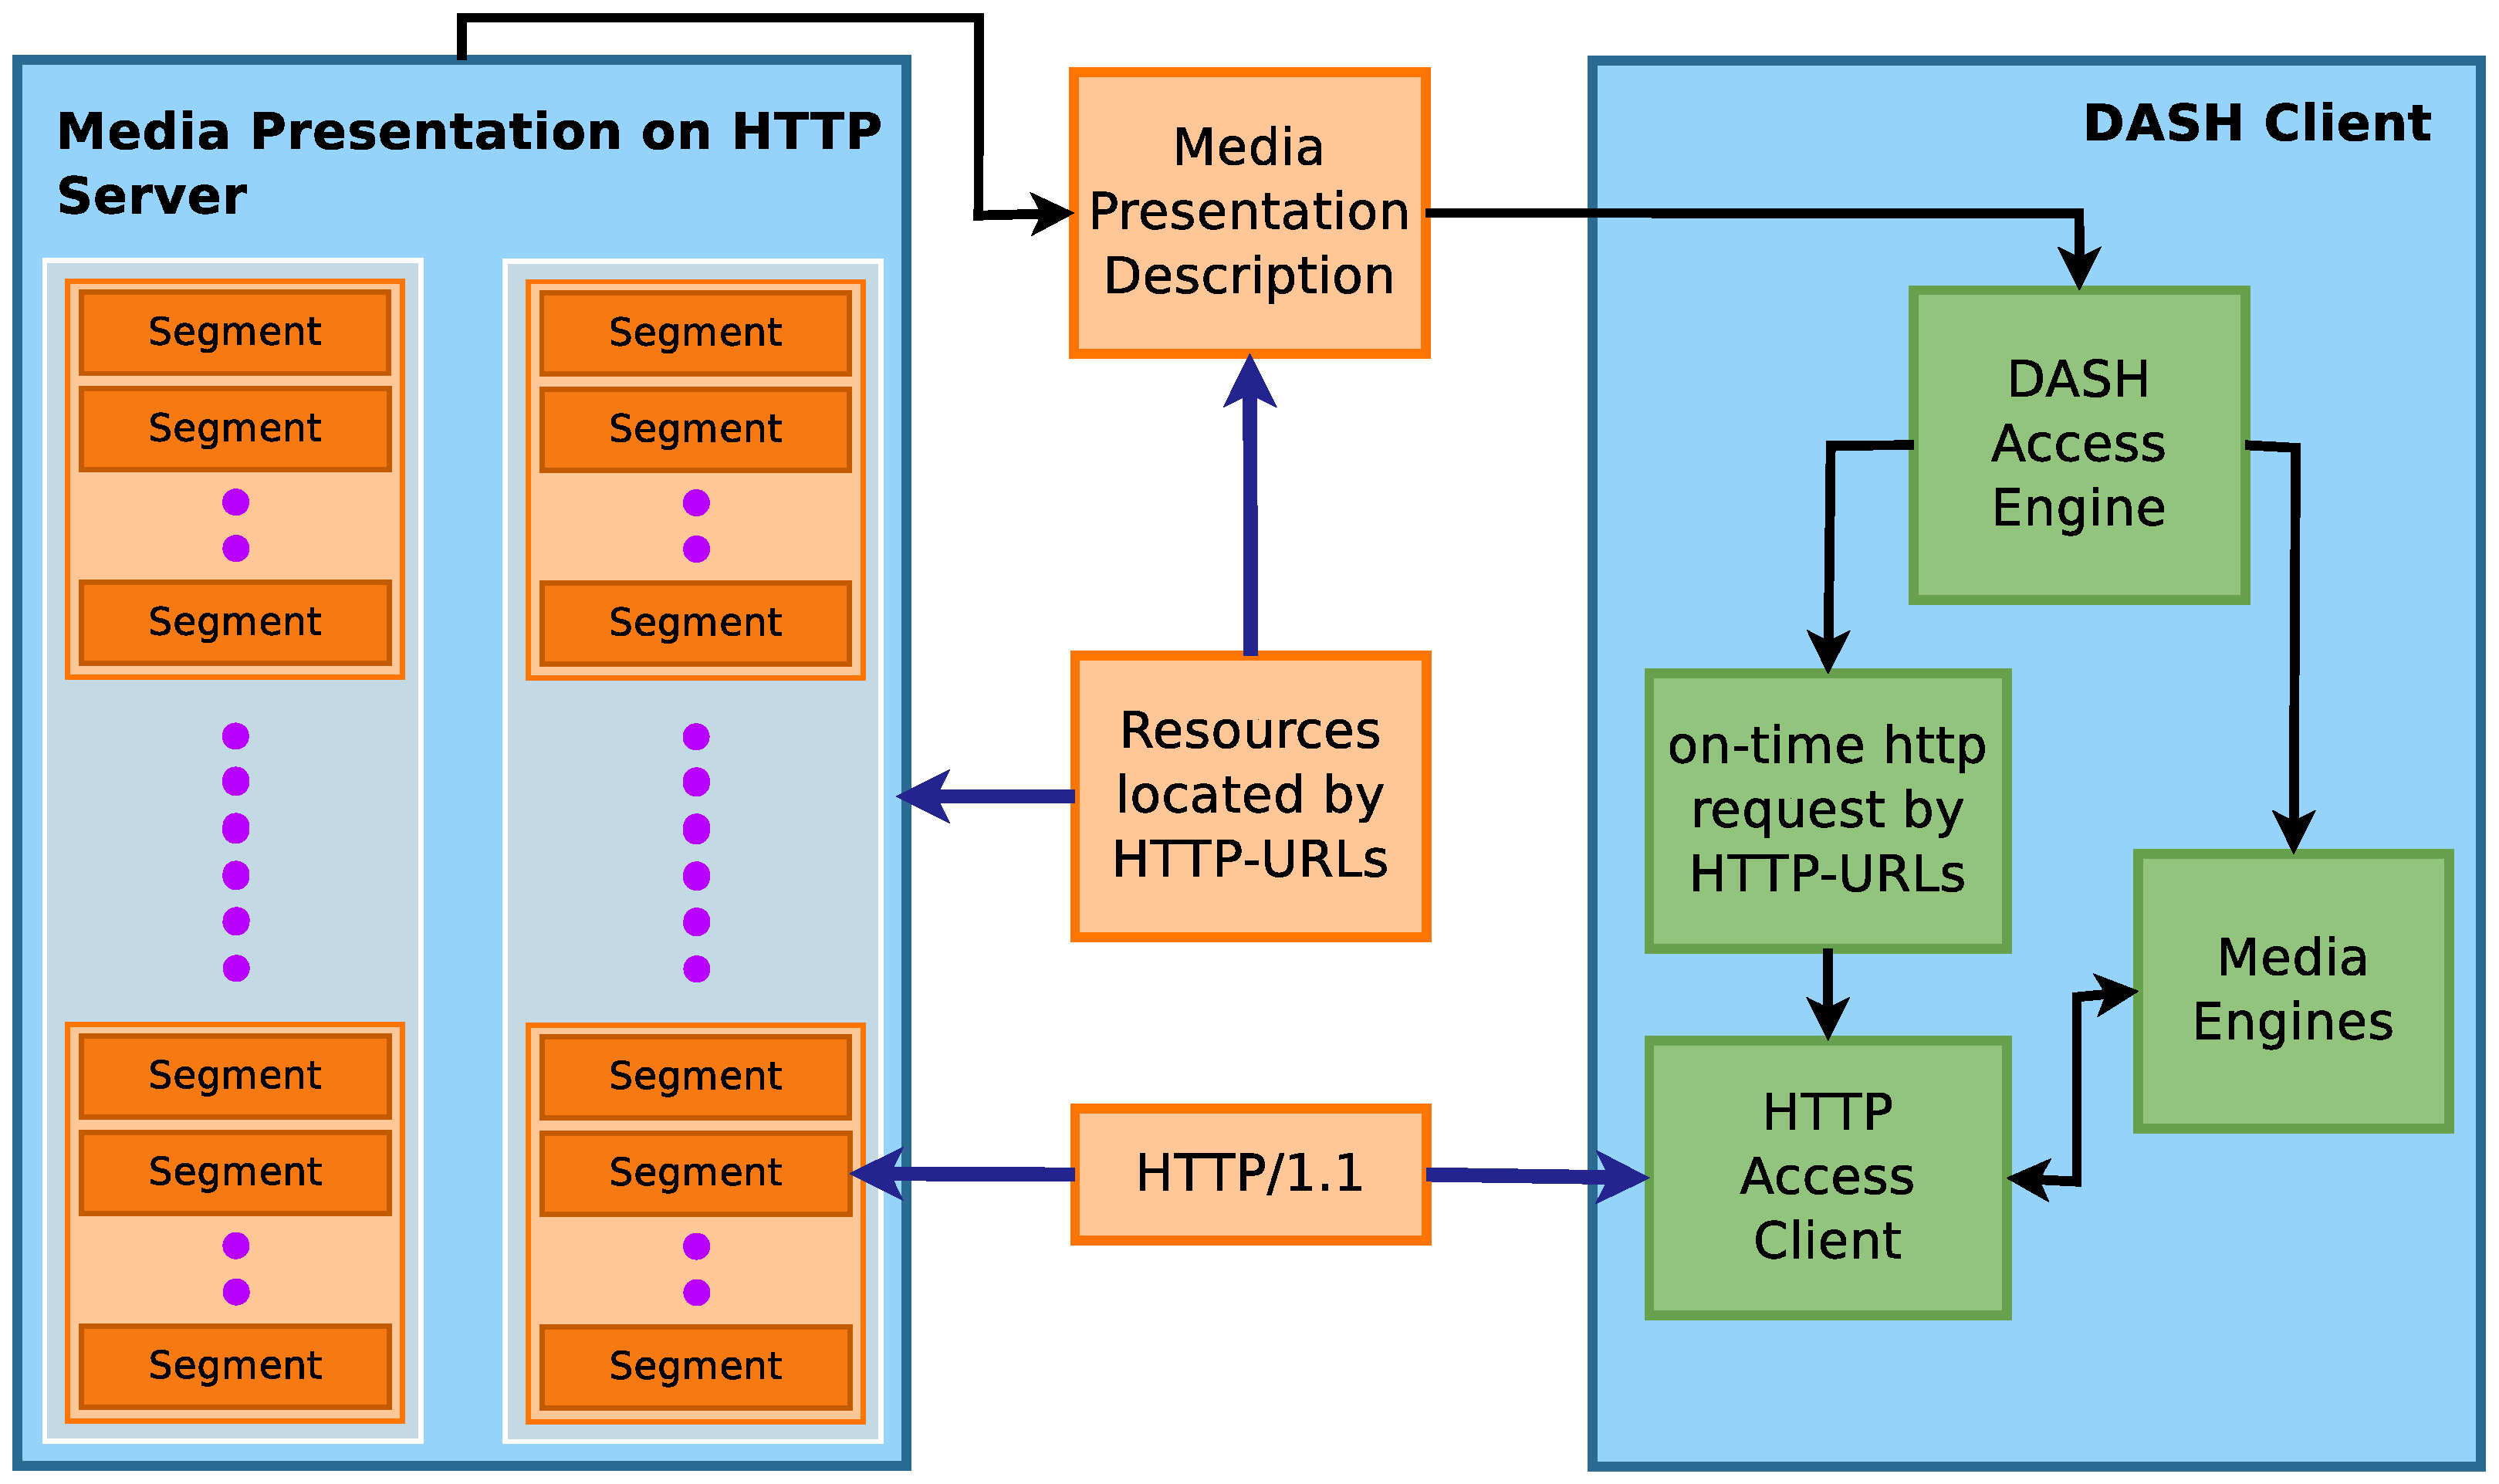
\includegraphics[scale=0.25]{img/dash-arch-old}
%	\caption{\small{DASH Architecture -- On the left side, the server-side media storage is shown, where content is divided into small segments of alternative bitrates. On the right side, the \acr{DASH} client architecture is shown; the {\it \acr{DASH} Access Engine} monitors the network bandwidth at the client and accordingly decides which segment to request from the server. (Image Source: https://www.w3.org/2011/09/webtv/slides/W3C-Workshop.pdf) (\lastaccessedtoday)}}
%	\label{fig:dash}
%\end{figure}
\begin{figure}[!t]
	\centering
	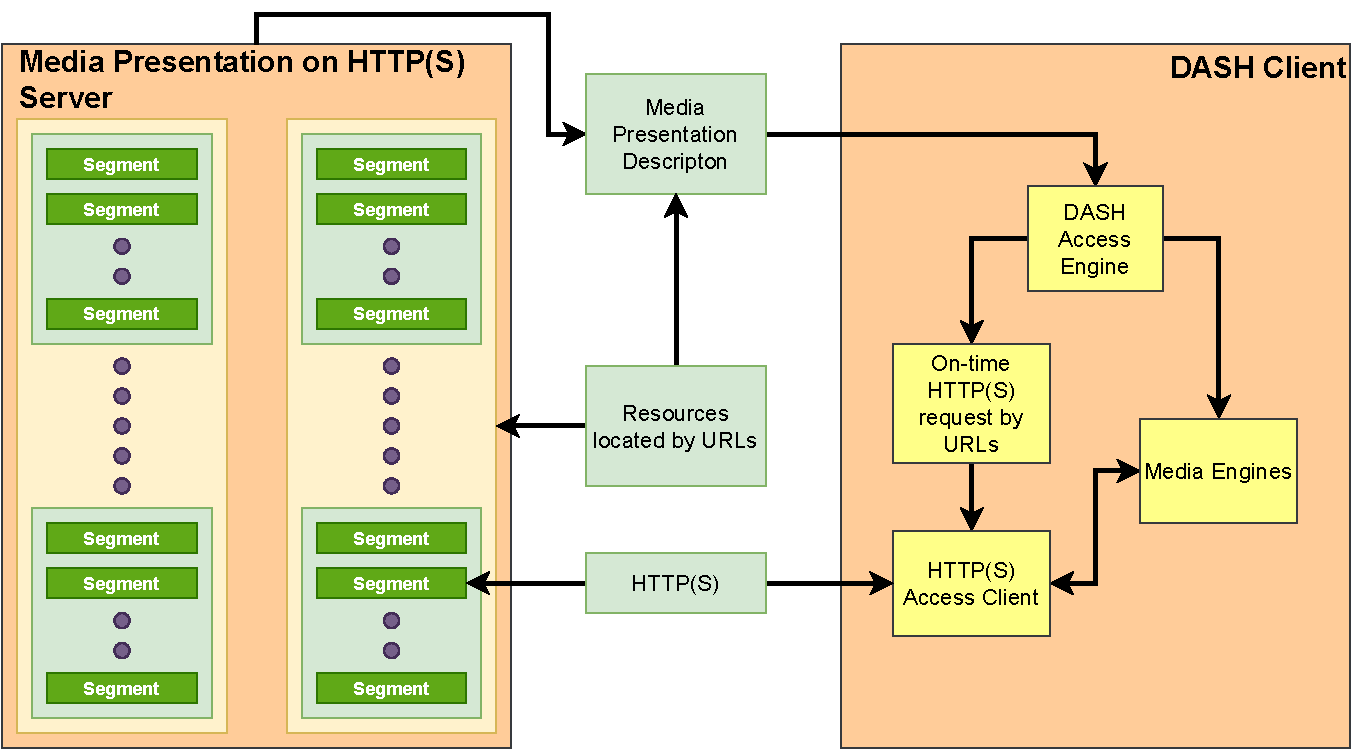
\includegraphics[width=\linewidth]{img/DASH-arch}
	\caption{\small{DASH Architecture -- On the left side, the server-side media storage is shown, where content is divided into small segments of alternative bitrates. On the right side, the \acr{DASH} client architecture is shown; the {\it \acr{DASH} Access Engine} monitors the network bandwidth at the client and accordingly decides which segment to request from the server.}}
	\label{fig:dash}
\end{figure}
In 2009, Apple developed the \ac{HLS} to replace the existing \ac{RTSP}-based video delivery for its QuickTime live streaming server\footnote{\url{https://appleinsider.com/articles/09/07/08/apple_launches_http_live_streaming_standard_in_iphone_3_0.html} (\lastaccessedtoday)}. \Ac{DASH}, sometimes calls as MPEG-DASH, is a technology developed under MPEG to stream videos over \acr{HTTP}. MPEG started working for DASH in 2010 and standardized it in 2011~\cite{ISO/IEC23009-1:2019}. After the release of {\tt dash.js} by \ac{DASH-IF}, almost all the streaming services, including YouTube, NetFlix, Samsung, etc., adopted \ac{DASH} in their services.

\fig{\ref{fig:dash}} shows the broad architecture of \ac{DASH}. Video streaming using DASH is a two-step procedure: a) preprocessing of the video files to distribute, and b) the streaming. 


\subsubsection{Video Preprocessing}
In the preprocessing (we also call it DASHifying) step, a streaming provider prepares the required files. It first splits the audio and video streams and encodes them into multiple bitrate versions. At this phase, the encoder needs to ensure that it aligns the I-frames\footnote{I-frame: a special type of frame that contains a complete picture and no-other frame required to render it. More details: \url{https://en.wikipedia.org/wiki/Video_compression_picture_types} (\lastaccessedtoday)} across different bitrate versions and places all the metadata at the beginning of the file. After encoding, three different types of files are created from the streams. These files are i) media index files, ii) media data files, and iii) a media presentation description file.

{\bf Media Index Files:} In general, when any media data is stored in a file, the file contains two pieces of information, a) the initialization part and b) the encoded media data. The initialization part contains information to decode the encoded data, which is the index for the original media data. The \ac{DASH} mandates that this initialization data should be stored in a separate file. So, while encoding a video into different bitrate versions, the metadata part needs to be kept at the starting of the output file. The index files are usually smaller than any of the media data, so it does not pose any overhead to the system.

{\bf Media Data Files:} The media data file contains the encoded media. According to \ac{DASH}, media data are segmented into multiple chunks with equal playback time. All the segments should have an I-frame at the beginning of the chunk.

{\bf \ac{MPD}:} It is an {\tt \acr{XML}} file that contains the metadata required to stream the video. It lists the different audio and video qualities available for streaming and the \acsp{URL} for the media index and media data. It also contains the codec, bitrate, and playback duration of individual chunks for each quality.

The preprocessing phase ends after storing all these different files in an \ac{HTTP(S)} file server. DASH does not require anything else on the server-side to stream a video. This is valid for both \ac{VoD} and live streaming. However, in live streaming, the segments are created on-the-fly and placed in the server before any client requests it.

\subsubsection{Video Streaming}
The second phase of the \acr{DASH}-based streaming is the video streaming. \ac{DASH} requires a smart player that can understand \ac{DASH} and play the video. Any \acr{DASH}-based video streaming starts by downloading the \ac{MPD} file. The player reads the \ac{MPD} file to get information regarding the video.  At this point, the player has to decide which quality it wants to play based on the \ac{ABR} algorithm running inside the player, and then it fetches the video chunks in the preferred quality. \ac{DASH} offloads the entire decision to the player so that any existing content delivery network can stream the video content. There are instances where media index files and media data are not chunked, instead kept in a fixed file. While this saves lot of disk space, the server has to support the HTTP range-request\footnote{\url{https://developer.mozilla.org/en-US/docs/Web/HTTP/Range_requests} (\lastaccessedtoday)}, and the player can get the desired chunk using the {\tt range} header.

\ac{DASH} also allows streaming providers to support various client platforms, encodes video in various codec and puts all the information in the \ac{MPD} file. Although the size of the \ac{MPD} file can be large, the player can choose a platform supported codec and play it without any hassle.


\subsection{Adaptive Bitrate Algorithms}
The adaptive bitrate algorithms are the heart of the DASH-based streaming system as it decides the quality of every video segment on-the-fly. By default, the \ac{ABR} algorithm runs just before fetching the next video segment to be downloaded. As the \ac{ABR} algorithm is a part of the player, it has access to all the playback related parameters, and it can use any of those parameters to decide quality for the next chunk. The primary goal of any \ac{ABR} algorithm is to maximize the \ac{QoE} so that users can enjoy the streaming.

\subsubsection{Quality of Experience (QoE)}
\ac{QoE} is a crucial parameter in any field which involves end-users. In the case of video streaming, \ac{QoE} is a metric to measure whether the user has enjoyed the video or not during the streaming. \ac{QoE} is mostly a metric of user perspective, and it depends on several factors such as the video startup delay, quality fluctuations, the overall quality, rebuffering, audio/video device, and video content. Although all these parameters are essential, it is not easy to measure user-dependent parameters and video content. Several researchers tried to design the best measurable metric to calculate the \ac{QoE}, which can be acceptable. Mok \etal \cite{5990550} tried to estimate \ac{QoE} from the network \ac{QoS}. They suggested that the user \ac{QoS} (or \ac{QoS} of \ac{HTTP}) is the \ac{QoE}. Various researches like \cite{10.1145/2155555.2155558,10.1145/3394171.3413512} tried to use \ac{PSNR} and \ac{SSIM} as a parameter for \ac{QoE}. Spiteri \etal\ considered only the rebuffering and the average quality as the \ac{QoE} in their \ac{ABR} algorithm BOLA~\cite{Spiteri2016}. Yin \etal~\cite{yin2015control} proposed an equation (\eqn{\ref{eqn:QoE}}) to calculate the \ac{QoE} using four parameters:
\begin{itemize}
	\item {\bf Video Startup Delay,} which is the delay before the playback can be started. In the case of \acr{ABR}-based solution, the startup delay depends on the efficient initial quality selection. Most of the \acr{ABR} algorithms ignore this parameter and set the initial quality as the lowest video quality available.
	\item {\bf Quality:} The sharpness of the video determines the quality of the video or audio. The sharpness of a video is directly related to the bitrate. It is expected that sharp media has better media details in both audio and video, thus providing a better experience in enjoying the stream. Any \ac{ABR} tries to maintain the bitrate as high as possible so that the \ac{QoE} improves.
	\item {\bf Smoothness:} \ac{DASH} allows the player to change the video quality on-the-fly. Frequent quality updates disrupt the smoothness of the video watching experience. So, \ac{ABR} needs to minimize the quality change during playback.
	\item {\bf Rebuffering:} Rebuffering is the most irritating experience for any user. The entire \ac{DASH} and \acr{DASH} like system is developed to minimize rebuffering during the video playback. The outmost responsibility of any \ac{ABR} algorithm is to minimize the rebuffering by selecting appropriate video quality, based of the current network quality.
\end{itemize}
\begin{equation}
\label{eqn:QoE}
QoE = \sum_{i=1}^N q(R_i) - \lambda\sum_{i=1}^{N-1}\left|q(R_{i+1})-q(R_i)\right| - \mu\sum_{i=1}^N \delta_i - \mu_s T_s
\end{equation}
\eqn{\ref{eqn:QoE}} is used by most modern \ac{ABR} algorithms which measure the \ac{QoE} for a video with $N$ segments, where $R_i$ represents the bitrate of $i^{th}$ segment, $q(.)$ is the utility function, $\delta_i$ is the stall before the $i^{th}$ segment ($\delta_0$ is always zero), $T_s$ is the startup delay. $\lambda$, $\mu$ and $\mu_s$ are constant weights to define importance of individual parameters.

To enhanced the online streaming experience, researchers have developed various systems and \ac{ABR} algorithms. We categorize the \ac{ABR} algorithms broadly in a) classical \ac{ABR} algorithms and b) learning based \ac{ABR} algorithms. In the following sections, we discuss both of these \ac{ABR} algorithms. Finally, we discuss the \ac{ABR} algorithms specially designed for live streaming and smartphones.



\section{Classical Adaptive Bitrate (ABR) Algorithm}
There are many classical ABR algorithms designed from the inception of DASH-like video streaming. Any classical ABR algorithm's primary goal is to run on a low-powered device without any external learning model. The classical ABR algorithms can be further categorized in {\tt buffer based}, {\tt throughput based}, {\tt hybrid} ABRs. We discuss a few ABR algorithms from each category in this section.

\subsection{Throughput based ABR algorithm}
Any ABR algorithm's primary job is to play video without rebuffering. To achieve this simple task, initially, ABR algorithms used to start with the lowest bitrate to quickly start the video and improve quality in subsequent segment until it detects some congestion or loss \cite{5677508,10.1145/1943552.1943575}. While this technique avoids rebuffering, it changes video quality for almost all the segment. Microsoft starts using a little more conservative solution in \cite{10.1145/1943552.1943574} while adapting bitrate based on the network quality. These algorithms have mitigated the rebuffering by matching the video bitrate with the observer instantaneous network throughput. However, they have failed to consider the fact that frequent change in quality can be an issue. These algorithms have the goal to improve the average quality and reduce the rebuffering. Later on, the ABR algorithms are designed to maintain the QoE. Few such algorithms are:

\subsubsection{QoE aware DASH (QDASH)}
Mok \etal\ designed the QDASH\cite{10.1145/2155555.2155558}, one of the early ABR algorithms with the awareness of QoE, consider that the abrupt quality changes are not acceptable. The algorithm has two parts, a) ABR algorithm and b) Bandwidth measurement tool. They proposed a particular module to run at the streaming server, which measures the client bandwidth. The ABR algorithm explicitly connects the measurement module and get in the bandwidth information. With the bandwidth information, QDASH finds the most suitable bitrate. However, QDASH does not switch to the most suitable bitrate immediately. Instead, it switches to the next bitrate to increase the QoE.

\subsubsection{Fair, Efficient, and Stable adapTIVE (FESTIVE)}
FESTIVE\cite{10.1145/2413176.2413189} is a DASH based video streaming system that provides fairness between players that share bottleneck stably and efficiently. Jiang \etal\ showed that the measured throughput might not be correct, and the available bottleneck bandwidth might be underutilized due to the scheduling scheme. So, they suggested a three steps method. These steps are:\\
a) Schedule the next segment download in a randomized manner so that every player gets a fair share of bottleneck links. \\
b) Select suitable bitrate based on last bandwidth estimation, but never jump bitrate instead of increasing one level at a time. \\
c) Estimate the available bandwidth as the harmonic mean of the last 20 throughput measurements.


\subsubsection{FEedback Linearization Adaptive STreamIng Controller (ELASTIC)}
All the client-side adaptive algorithms generate an ON-OFF traffic pattern, which led to unfairness among the players. Cicco \etal\ designed ELASTIC\cite{6691442}, a client-side controller that does not generate ON-OFF traffic pattern. ELASTIC select video bitrate for a segment in such a way so that it finishes downloading the segment at the time when the next segment needs to be downloaded. So, there is no requirement for the ON-OFF traffic generation, and traffic can be fair as underlying TCP is fair for the long-running flows.

\subsubsection{Presto: fair and efficient streaming using multiple servers}
Zhang \etal\ designed Presto\cite{7249417}, which provides fairness among the players that stream video from multiple servers. They argue that a player might consume more bandwidth of the bottleneck by running more parallel flows. So, they provide a mechanism to restrict a player's bitrate with more flows and improve quality. Presto exploits the fact that a user gets annoyed with drastic bitrate drop; however, not with drastic bitrate increase\cite{10.1145/2018602.2018611}. It also suspends some flows to stabilize the bandwidth utilization for the time and resume later.

\subsubsection{Spectrum-based QUality ADaptation (SQUAD)}
SQUAD\cite{10.1145/2910017.2910593} is a spectrum\cite{1386243} based quality adaptation technique for DASH based video streaming system. Wang \etal\ assumed spectrum as the variation in the bitrate around some $N$ number of segments. The proposed system starts with providing a new method to measure the throughput. Typically throughput is measured when a segment is completely downloaded, and estimations are made based on the past throughput measurement. The authors have pointed out that this technique may not be correct as the sizes of the segments are different, and thus it might take different times to download different segments even if the bandwidth is the same. So, SQUAD suggested performing a running average of throughput over the course of a segment downloading. It proposed to set the bitrate of a few initial segments to the lowest bitrate available and, after the initial set of segments, set bitrate in such a way so that the bitrate variation in a window, i.e., SPECTRUM, is the lowest.


\subsection{Buffer Based}
The buffer-based bitrate adaptation technique is an alternative technique of throughput based where the player does not need to estimate or measure the throughput to adapt the playback quality as the throughput estimation is complex and most of the time inaccurate due to the nature of network dynamics. Also, middleboxes like catching devices, including proxy, make it more difficult to estimate real throughput. Buffer-based ABR algorithms do not suffer from a similar problem. In the past decade, researchers have designed several buffers based ABR algorithms. We are going to discuss a few of those algorithms.

\subsubsection{Buffer based rate adaption}
Huang \etal\ (\cite{Huang2014,10.1145/2398776.2398800,10.1145/2491172.2491179}) described a bitrate adaptation mechanism solely based on the playback buffer level. The author suggested that the playback buffer is a function of bitrate and network throughput. Thus player buffer level can be an indication of whether to change bitrate or not. Authors use a rate to buffer map to calculate the bitrate for a given buffer. They use an algorithm to remove any fine boundary between bitrates to avoid frequent bitrate fluctuations.

\subsubsection{Threshold driven buffer based adaptation}
Miller \etal\ designed a buffer based algorithm in \cite{6229732} as an remedy for the measurement problem of throughput driven algorithms. They uses 3 buffer levels, $B_{min}$, $B_{low}$ and $B_{max}$ ($0 < B_{min} < B_{low} < B_{max}$) as threshold to decide the bitrate switch. The algorithm aims to keep the buffer level to close to mean of $B_{low}$ and $B_{max}$. It decrease the bitrate if buffer level goes below $B_{low}$, drops to lowest if it goes below $B_{min}$ and increase if it goes beyond $B_{max}$.

\subsubsection{Smooth Adaptive Bit RatE (SABRE)}
SABRE is designed to mitigate TCP's buffer bloat effect, which might cause queuing delay up to a few seconds. Mansy \etal(\cite{10.1145/2483977.2484004}) suggested using the HTTP pipeline where multiple HTTP-request can be pushed together. At the client-side, make {\tt recv} call in a non-aggressive way to reduce the queuing delay as it prevents the sender side from pushing excessive data. Due to its paced {\tt recv} call, it is impossible to measure throughput correctly. So, it changes the pacing of {\tt recv} call based on the playback buffer. The player changes the bitrate as per the observed download rate, which is governed by the non-aggressive pacing.

\subsubsection{Buffer Occupancy based Lyapunov Algorithm (BOLA)}
BOLA\cite{Spiteri2016} treat ABR streaming as an optimization problem where the average bitrate needs to maximize, and rebuffering needs to be minimized. Spiteri \etal\ solved the problem using Lyapunov optimization and provided a theoretical guarantee on the QoE. BOLA does not require any estimation of the throughput. Instead, it is solely based on the playout buffer.

\subsubsection{Adaptation \& Buffer Management Algorithm (ABMA+)}
Beben \etal\ proposed ABMA+\cite{10.1145/2910017.2910596} which predicts the video freezing probability for each representation and selects the best representation satisfies the predefined freezing probability threshold. It continuously monitors the segment download time and uses time characteristics, and the precomputed buffer-map decides the best bitrate for smooth playback.

\subsubsection{Markov Decision-Based Rate Adaptation Approach (mDASH)}
mDASH\cite{7393865} formulate rate adaptation problem as Markov Decision Process (MDP)\cite{P-1066} optimization. According to Zhou \etal\, the state vector define the system state, including buffer occupancy, playback rate, previous video bitrate, network bandwidth. The action is the bitrate for the next segment. They calculate reward based on various parameters that affect the visual quality, including quality, quality switch frequency and magnitude, and rebuffering. The optimization problem is difficult to solve directly as there are many uncertainties during the streaming session due to time-varying network conditions, so the authors proposed a sub-optimal greedy solution to solve the problem. According to their evaluation mDASH perform at per with the optimal solution.

\subsection{Hybrid ABR algorithms}
Some ABR algorithms consider both buffer and throughput to adapt the bitrate. These algorithms can be further categorized in control system based and without control system based. We will discuss few of them here.

\subsubsection{Smooth rate adaptation}
The authors of \cite{10.1145/2413176.2413190} and \cite{6694183} proposed a method involving a control loop and measured throughput and playback buffer. The control loops start with a playback buffer and a reference buffer, and the difference between these two is used to predict the throughput. Then the predicted throughput is used to determine the video bitrate. The video bitrate and the real throughput lead to playback buffer occupancy, further used in the control loop.

\subsubsection{Probe and Adapt (Panda)}
Li \etal\ (\cite{140405}) found that most of the widely deployed DASH like streaming suffers from bitrate fluctuation when multiple players share a bottleneck. They also found that the fluctuation depends on various parameters, including the number of players, players' start time, and background traffic. While digging more, they found that all the techniques assume that the measured throughput is fair and can be used directly. However, it is not true and due to this fundamental mistake player lost the capability of over-coming buffer underrun. Li \etal\ suggested using probe the network to find the available bandwidth. PANDA uses TCP like the AIMD scheme for rate-adaptation. However, it only uses the probe per chunk instead of per RTT.

\subsubsection{Segment Aware Rate Adaptation (SARA)}
SARA\cite{7247436} is a segment aware rate adaption technique developed by Juluri \etal. It is a hybrid adaptive system where the playback buffer is used to decide how the bitrate should change, and the throughput is used to decide the appropriate bitrate. It has bitrate adaptation scheme based on four buffer thresholds. These are a) slow-start: when buffer ($B_{curr}$) very low ($B_{curr}<I$), lowest bitrate is selected, b) additive increase: when buffer is moderated ($B_{\alpha} \le B_{curr} > B_{\beta}$), it carefully increase the bitrate and c) aggressive bitrate switching: if the buffer is high enough ($B_{\beta} \le B_{curr} \ge B_{max}$, bitrate can jump without any effect and d) delayed download: if the buffer is saturated ($B_{max} < B_{curr}$), download have to wait for buffer goes down.

\subsubsection{Model predictive control algorithm}
Model predictive control (MPC) algorithm is proposed by Yin \etal\ in their paper \cite{yin2015control,10.1145/2670518.2673877} as superior ABR algorithm than the existing algorithms by optimally combine the throughput and buffer occupancy information. The authors formulated the QoE optimization problem as a stochastic optimal control problem and tried to solve it using MPC. They formulate the bitrate selection as a function of three components a) predicted future bitrate, b) buffer occupancy, and c) available bitrates. The basic MPC algorithm is made up of three steps: \\
a) Predict: Although the future throughput prediction is difficult most of the time inaccurate, it assumes that there is a way to do it with acceptable errors. In the throughput prediction step, they can use any third party algorithm to predict the throughput.\\
b) Optimize: In this phase, the MPC search for the bitrate for next $N$ segments with predicted throughput and calculated buffer occupancy and choose the best one. The problem can be solved using {\tt CPLEX} solver.\\
c) Apply: Once bitrate is selected, it should start downloading the segment.\\
The optimization step is computationally heavy, and it has to perform before downloading each segment. So, the authors have proposed an alternative to do it fast by using lightweight combinations.


\subsubsection{Fine-Grained Video Rate Adaptation (Favor)}
Fine-grained Video Rate Adaptation or Favor\cite{10.1145/3204949.3204957} proposed by the He \etal\ to optimize the non-conventional parameters like frame-dropping rate, playback speed along with convention parameter bitrate to optimize DASH based player beyond the optimization horizon. The author suggested that the viewer cannot notice up to 35\% frames drops as well as up to 25\% reduction in playback speed. Although these changes are non-conventional, it can allow the player to cope with the throughput reduction as frame reduction cause the segment size reduction, and playback rate reduction gives more time to download segment. Favor also suggest a framework for 360$^{\circ}$ video by tiling and optimizing individual tiles.

\subsubsection{DASH with P2P}
Yousef \etal\ designed a technique in their paper \cite{10.1145/3339825.3391859} to allow any ABR algorithm to work in a hybrid CDN+P2P DASH based video streaming system. They suggested keeping the video player and the P2P module separate so that any DASH based ABR algorithm can be applied to the player. The authors have found out the main problem with P2P DASH based streaming as the estimation of throughput or buffer filling rate as the throughput and delay vary drastically depending on whether it is downloading from CDN or a nearby peer. It maintains the player observed throughput steady by adding extra delay in their P2P module while downloading segments from a nearby peer. This way, any DASH based ABR algorithm can work in player.

\subsection{Summary}
In summary, there are several classical ABR's developed over the years. It starts with simple throughput driven ABR algorithms, where ABR directly match the streaming quality to the last observed network throughput \cite{5677508,10.1145/1943552.1943575,10.1145/1943552.1943574}. Although it reduces the rebuffering, quality change is imminent. So researchers try to tun the throughput measurement and quality switching policy to improve QoE. However, throughput-based algorithms require continuous throughput measurement, which is not possible due to the ON-OFF traffic pattern. Also, the fine-grain throughput measurement is not possible from the application layer due to the network stack's nature. So, researchers start developing buffer based ABR algorithm as the buffer can be an indication of throughput. Buffer based algorithms adapt bitrate with or without bitrate map. The frequent quality switch is still a problem. So both throughput based and buffer based algorithms uses a special algorithm to avoid strict change in quality.

While throughput and buffer-based ABR algorithms provide reasonably better QoE, there are places to improve. It cannot always provide the best solution due to the nature of the network dynamics—Hybrib solution can rescue ABRs from those pitfalls. ABR algorithms in \cite{7247436,140405,yin2015control,10.1145/2670518.2673877} performs much better than any buffer based or throughput based algorithms. These algorithms assume the QoE maximization as an optimization problem and try to solve it. However, there are problems in deploying hybrid ABR algorithms as these are complex, computationally heavy, and require a special solver to solve the problem. Although algorithm designers usually provide a lightweight solution, those are not adequate.

All the existing ABR algorithms have some advantages as well as disadvantages. We compare those algorithms in terms of a few basic parameters in Table~\ref{chap02:tbl:comparison_classical}.

% Please add the following required packages to your document preamble:
% \usepackage{multirow}
\begin{table}[h!]
	\resizebox{\textwidth}{!}{
	\begin{tabular}{|l|cccc|c|c|l|}
		\hline
		\multicolumn{1}{|c|}{\multirow{3}{*}{Algorithm}} & \multicolumn{4}{c|}{Goal involved} & \multirow{3}{*}{\begin{turn}{90}No Extra Module\end{turn}} & \multirow{3}{*}{\begin{turn}{90}Continuous Traffic\end{turn}} & \multicolumn{1}{c|}{\multirow{3}{*}{Remark}} \\
		\cline{2-5}
		& \begin{turn}{90}Rebuffering\end{turn} & \begin{turn}{90}Quality\end{turn} & \begin{turn}{90}Smoothness\end{turn} & \begin{turn}{90}Fairness\end{turn} & & & \\
		& & & & & & & \\
		\hline
		\multicolumn{8}{|c|}{Throughput Based}\\
		\hline
		QDASH\cite{10.1145/2155555.2155558} & \green{\cmark} & \green{\cmark} & \green{\cmark} & \red{\xmark} & \red{\xmark} & \red{\xmark} & Match observed bitrate \\
		FESTIVE\cite{10.1145/2413176.2413189} & \green{\cmark} & \green{\cmark} & \green{\cmark} & \green{\cmark} & \green{\cmark} & \red{\xmark} & \begin{tabular}[c]{@{}l@{}}Harmonic Mean\\ No bitrate jump\end{tabular} \\
		ELASTIC\cite{6691442} & \green{\cmark} & \green{\cmark} & \red{\xmark} & \green{\cmark} & \green{\cmark} & \green{\cmark} & Fairness from long running TCP \\
		Presto\cite{7249417} & \green{\cmark} & \green{\cmark} & \green{\cmark} & \green{\cmark} & \green{\cmark} & \red{\xmark} & Multi-flow down stream per player \\
		SQUAD\cite{10.1145/2910017.2910593} & \green{\cmark} & \green{\cmark} & \green{\cmark} & \red{\xmark} & \green{\cmark} & \red{\xmark} & \begin{tabular}[c]{@{}l@{}}Specturm based\\ Running average throughput\end{tabular} \\
		\hline
		\multicolumn{8}{|c|}{Buffer Based}\\
		\hline
		Buffer based rate Adaptation\cite{Huang2014,10.1145/2398776.2398800,10.1145/2491172.2491179} & \green{\cmark} & \green{\cmark} & \red{\xmark} & \red{\xmark} & \green{\cmark} & \red{\xmark} & rate2buffer map \\
		Threshold Based\cite{6229732} & \green{\cmark} & \green{\cmark} & \red{\xmark} & \red{\xmark} & \green{\cmark} & \red{\xmark} & Buffer threshold decides bitrate \\
		SABRE\cite{10.1145/2483977.2484004} & \green{\cmark} & \green{\cmark} & \red{\xmark} & \red{\xmark} & \green{\cmark} & \red{\xmark} & Avoids buffer bloat \\
		BOLA\cite{Spiteri2016} & \green{\cmark} & \green{\cmark} & \red{\xmark} & \red{\xmark} & \green{\cmark} & \red{\xmark} & Theoretical Guarantee on video quality \\
		ABMA+\cite{10.1145/2910017.2910596} & \green{\cmark} & \green{\cmark} & \green{\cmark} & \red{\xmark} & \green{\cmark} & \red{\xmark} & Buffer freezing probability threshold \\
		mDASH\cite{7393865} & \green{\cmark} & \green{\cmark} & \green{\cmark} & \red{\xmark} & \green{\cmark} & \red{\xmark} & MDP optimization problem \\
		\hline
		\multicolumn{8}{|c|}{Hybrid} \\
		\hline
		Smooth rate adaptation\cite{10.1145/2413176.2413190,6694183} & \green{\cmark} & \green{\cmark} & \red{\xmark} & \red{\xmark} & \green{\cmark} & \red{\xmark} & \begin{tabular}[c]{@{}l@{}}Control look\\ Throughput prediction\end{tabular} \\
		PANDA\cite{140405} & \green{\cmark} & \green{\cmark} & \green{\cmark} & \green{\cmark} & \green{\cmark} & \red{\xmark} & \begin{tabular}[c]{@{}l@{}}Probe network by increased datarate\\ AIMD bitrate selection\end{tabular} \\
		SARA\cite{7247436} & \green{\cmark} & \green{\cmark} & \red{\xmark} & \red{\xmark} & \green{\cmark} & \red{\xmark} & \begin{tabular}[c]{@{}l@{}}Buffer used to decide selection algo\\ Match measured throughput\end{tabular} \\
		MPC\cite{yin2015control,10.1145/2670518.2673877} & \green{\cmark} & \green{\cmark} & \green{\cmark} & \red{\xmark} & \green{\cmark} & \red{\xmark} & Assume throughput is predictable \\
		FAVOR\cite{10.1145/3204949.3204957} & \green{\cmark} & \green{\cmark} & \green{\cmark} & \red{\xmark} & \red{\xmark} & \red{\xmark} & \begin{tabular}[c]{@{}l@{}}Changes playback speed\\ Drop frames\end{tabular}\\
		\hline
	\end{tabular}
	}
	\caption{\label{chap02:tbl:comparison_classical}Comparisons of classical ABR algorithms}
\end{table}


\section{(Machine) Learning-based ABR algorithms}
We discussed various algorithms that use instantaneous parameters like buffer occupancy and throughput to decide the segment's bitrate. However, researchers have also developed a learning-based algorithm to solve the problem. In this section, we discuss some of those algorithms.

\subsection{Multi-agent Q-Learning}
Petrangeli \etal\ proposes Multi-agent Q-Learning\cite{6838245}, a reinforcement-learning based ABR algorithm. The algorithm does not change the client-side architecture. However, add a co-ordinating proxy server between the server and client. The proxy server collects and aggregates the reward from all the players. Then it computes the global signal from the reward and broadcasts to the players. The global signal is used to compute the Homo Egualis\cite{10.5555/1402298.1402344} reward, which is used to provide fairness among the players. With this Homo Egualis reward, players can compute the local reward, which in turn leads to the selection of video quality with the help of throughput, segment lengths, and quality levels.

\subsection{Markov Decision Process optimization}
Gadaleta \etal(\cite{8048013}) and Chiariotti \etal(\cite{10.1145/2910017.2910603}) formulate the Adaptation problem as Markov Decision Process (MDP)\cite{P-1066} optimization problem. Authors have found out that the future state of the process solely depends on the present state. Here, the system's state is defined as quality level, available throughput, size of the segment, and the playback buffer. The state transition happened based on the action taken in the current state based on the action, which is essentially the bitrate. The reward was calculated based on the previous state, action taken in the previous state, and current state. Chiariotti \etal\ use online reinforcement learning to solving the problem to make the best possible decision while Gadaleta \etal\ uses Q-Learning-based deep-neural network to the solve the same problem.

%\subsection{Deep Q-Learning based DASH (D-DASH)}
%D-DASH\cite{8048013} is a deep-neural network-based ABR solution. Like \cite{10.1145/2910017.2910603}, Gadaleta \etal\ formulate the problem as MDP optimization. However, the authors suggested a Q-Learning-based deep-neural network solution instead of an RL-based solution as it is compact and fast.

\subsection{Pensieve}
Mao \etal\ designed Pensieve\cite{mao2017neural} to solve the bitrate selection problem using Recurrent Neural Network. The Pensieve treats multiple parameters, including buffer occupancy, download history, playback time as the current state, and bitrate selection as the action to move to the next state. Pensieve uses the QoE as the reward for state transition. The aim here is to increase the reward, i.e., QoE, by taking accurate action. Pensieve selection action based on the policy, which a probability distribution of state and action pair. As there are intractably many such pair exists, Pensieve uses a neural network to represent the policy with manageable parameters. It uses the actor-critic neural-network to train the policy with the policy gradient method\cite{sutton1999policy}. It also uses the A3C\cite{10.5555/3045390.3045594} algorithm, an actor-critic method involving two networks, to train its model.\\
Pensieve proposes a simulation-based method to train the network fast, and then the trained model is then used in the real playback system. To make the training process even faster, they propose asynchronous parallel training involving primary and secondary networks.

\subsection{Auto-tuning Video ABR Algorithm (Oboe)}
Oboe\cite{Akhtar2018} is another learning-based ABR technology devised by Akhtar \etal. While Oboe does not directly provide any algorithm to select bitrate for each segment, it tunes the configuration of other ABR algorithms including MPC\cite{yin2015control,10.1145/2670518.2673877}, BOLA\cite{Spiteri2016} and Penseive\cite{mao2017neural} based on the network state. Oboe precomputes the appropriate configuration settings for any algorithm based on the different network states using reinforcement learning. It applies the learned model online to tune the configuration to provide the best possible outcome by an ABR algorithm.


\subsection{Periodical Experience Replay for Multi-path (PERM)}
PERM\cite{9155492} is an actor-critic network-based neural adaptive video streaming system that can exploit the multipath capability of multi-homing devices developed by Guan \etal. PERM uses one actor-network to decide the quality for a segment and another for deciding the path to fetch that segment and uses only one critic-network to evaluate the decision.

\subsection{Super-Resolution based video streaming}
Zhang \etal\ presented a novel approach to increase video streaming quality in their paper \cite{9155384} by improving video quality by the technique call Super-Resolution. Video super-resolution is a technique to reconstruct high-resolution frames from consecutive low-resolution frames. The use RL-based decision engine to decide the download resolution and whether reconstruction is require or not. The RL-based decision engine is designed based on state of the actor-critic network.

\subsection{LiveClip}
Most of the ABR algorithm improve video quality for long video, and they start with lowest possible video quality. Although it is okay for long video as initial part usually not that important, it is problem for short videos. Infact there are services to stream very short videos. LiveClip\cite{10.1145/3386290.3396937} solves the problem by designing a deep reinforcement learning-based ABR algorithm for short videos. He \etal\ consider a special scenerio where user can scroll through the page to change video and video needs to played when ever it in the visual section. They use adaptive streaming for entire session instead of per video and adaptation done based on the application session (i.e. multiple video in a session).

\subsection{Overhead-aware Adaptive Video Streaming (Grad)}
Grad\cite{10.1145/3394171.3413512} is overhead-award ABR for SVC based video streaming. By default, DASH is not designed for SVC based video streaming, so most of the ABR algorithm does not support DASH. Also, SVC involves a lot of extra overhead in decoding. Liu \etal\ design grad to mitigate those problems. To reduce decoding overhead, they propose {\tt jump enabled hybrid coding} where only one enhancement layer can be used to jump multiple SVC layers. On top of this optimization, they use actor-critic network-based reinforce-learning to adapt the quality.

\subsection{Summary}
Machine learning and deep learning can perform better than classical system if trained correctly. The ABR algorithm like Pensieve, Oboe, show the potential of the machine learning algorithm. The idea of super-resolution and liveClip give another perspective to the video streaming paradigm. While all these ABR algorithms work well with in the evaluation there are not easy to deploy widely. Most the ABR algorithm needs to train for a long time before they can be used. The training time is huge and computationally heavy. Training needs to done frequently and some per video. Another big hurdle in the deployment of the these algorithm is the library dependency. To infer correct decision from the a ML require library support and all the different platform specially smartphone platform does not support all the libraries. Inference can be made by offloading computation to a server, however, it is extreamly inefficient as it involve the network. We fill there is much work needed before any of the algorithm can be deployed widely and efficiently.

\begin{table}[h!]
	\resizebox{\textwidth}{!}{
		\begin{tabular}{|l|cccc|c|c|l|l}
			\hline
			\multicolumn{1}{|c|}{\multirow{3}{*}{Algorithm}} & \multicolumn{4}{c|}{Goal involved} & \multirow{3}{*}{\begin{turn}{90}No Extra Module\end{turn}} & \multirow{3}{*}{\begin{turn}{90}Continuous Traffic\end{turn}} & \multicolumn{1}{c|}{\multirow{3}{*}{Remark}} \\
			\cline{2-5}
			& \begin{turn}{90}Rebuffering\end{turn} & \begin{turn}{90}Quality\end{turn} & \begin{turn}{90}Smoothness\end{turn} & \begin{turn}{90}Fairness\end{turn} & & & \\
			& & & & & & & \\
			\hline
			Multi-agent Q-Learning & \green{\cmark} & \green{\cmark} & \green{\cmark} & \green{\cmark} & \red{\xmark} & \red{\xmark} & \begin{tabular}[c]{@{}l@{}}Reinforcement Learning\\ Coordination proxy required\end{tabular} \\
			RL-based Online Learning & \green{\cmark} & \green{\cmark} & \green{\cmark} & \red{\xmark} & \green{\cmark} & \red{\xmark} & \begin{tabular}[c]{@{}l@{}}Markov decision process\\ Reinforcement learning to solve MDP\end{tabular} \\
			D-DASH & \green{\cmark} & \green{\cmark} & \green{\cmark} & \red{\xmark} & \green{\cmark} & \red{\xmark} & \begin{tabular}[c]{@{}l@{}}Markov decision process\\ Deep neural network solve MDP\end{tabular} \\
			Pensieve & \green{\cmark} & \green{\cmark} & \green{\cmark} & \red{\xmark} & \green{\cmark} & \red{\xmark} & \begin{tabular}[c]{@{}l@{}}Policy gradient training\\ A3C based actor-critic network\\ Simulation based training\end{tabular} \\
			Oboe & \green{\cmark} & \green{\cmark} & \green{\cmark} & \red{\xmark} & \green{\cmark} & \red{\xmark} & Configuration tuning \\
			PERM & \green{\cmark} & \green{\cmark} & \green{\cmark} & \red{\xmark} & \green{\cmark} & \red{\xmark} & \begin{tabular}[c]{@{}l@{}}Path selection problem\\ Actor-critic network with two actor network\end{tabular} \\
			Super-resolution & \green{\cmark} & \green{\cmark} & \green{\cmark} & \red{\xmark} & \red{\xmark} & \red{\xmark} & \begin{tabular}[c]{@{}l@{}}Post download quality enhancement\\ Neural network based solution\end{tabular} \\
			\hline
		\end{tabular}
	}
	\caption{\label{chapter02:table:comparison_ml}Comparisons of machine-learning based ABR algorithms}
\end{table}


\section{Adaptive Live Streaming}
\label{chapter02:live}
DASH-like video streaming system is widely used as it is superior to other systems, and live video streaming is no exception. Although interactive video sessions are difficult to support via DASH due to the rigid latency bound, non-interactive live video streamings are well supported. Static (or VoD) and live video streaming are almost identical as per player perspective, except that live streaming does not support video seeking. However, providing live streaming is not easy as all the segments need to be captured, processed, and distributed to the nearest server before it can be served to the client. All these tasks need to be performed with reasonably small delay; otherwise, the user experience might degrade. Researchers have developed various systems to reduce the delay and scale of the live streaming to millions of users.

\subsection{Crowdsourced Live Streaming}
Live video streaming requires live transcoding into multiple different quality versions and different codecs to support a large set of platforms with higher QoE. Unlike TV broadcasting, live streamings are mostly crowdsourced. The crowdsource streamer and viewers are geo-distributed and use heterogeneous platforms. The streaming service provider needs to support all those kinds of streamers and viewers and provide the best possible QoE. Chen \etal\ explored the possibility of locating a suitable transcoding server as per the geolocation of streamer and viewer with the help of cloud federation in their research paper~\cite{7218642}.

Even though the cloud can be used to transcode live streaming effectively, it is not always economical as not all the videos are equally popular, and clients may not use all the quality and codec versions. However, transcoding in multiple codec and quality is expensive computationally as well as economically. So streaming providers need to be careful about the selection of the codec and quality level they support for each live streaming. Aparicio-Pardo \etal\ have designed an Integer Linear Programming (ILP)-based algorithm in their paper \cite{10.1145/2713168.2713177} to decide the number of quality levels required for live streaming, based on the streaming characteristics and popularity. It decides the CPU (GPU) budget for each live stream and decides the quality levels. 


\subsection{SmoothCache 2.0}
To reduce the distribution overhead, server load, and improve the quality of experience during the live streaming, SmoothCache~2.0~\cite{10.1145/2713168.2713182} provides a solution involving P2P networking with DASH. Roverso \etal\ have exploited the fact that all the live streaming players need to be in sync with very little tolerance $\delta$. The $\delta$ is the time when a player searches for the required segment in other peers and, if failed, fetches it from the CDN. The authors have used optimizations like pro-active prefetching to reduce the overhead. Pro-active prefetching allows few players to fetch the segment as soon as they become available at the server.

\subsection{Neural-Enhanced Live Streaming (LiveNAS)}
QoE of a live stream is dependent on the network quality and computation capability, especially when random individual users start streaming using commodity devices like a smartphone with a cellular data connection. Due to the lack of dedicated Internet connection and lack of infrastructure, these users can not ensure a steady streaming quality. Kim \etal\ have designed LiveNAS~\cite{10.1145/3387514.3405856} to improve video quality in such cases. LiveNAS runs super-resolution to upgrade video quality at the ingest server if the uploaded video quality drops during the playback.

\subsection{Summary}
Live video streaming is apparently similar to the VoD video streaming system. However, live streaming needs server side support for live content generation and distribution. This task is fairly complex if a streaming provider wants to support crowdsourced live streaming. They have to allocate resources to encode and distribute the video content. On the other hand, live streaming of mega-event attracts millions of viewers globally. Existing literature tries to scale the distribution network by utilizing P2P networks. Work like \cite{10.1145/2713168.2713182} have tried to utilize the peer-to-peer network to share video segments among players. However, it may not work well if players have to use the Internet uplink to share the video segment, as uplink speeds are usually low and count towards their data cap. We believe that there is scope to improve live streaming as many live streaming video players share the same Internet connections.

\section{Video Streaming over Smartphones}
The availability of cheap data plan over the LTE network and the availability of contents in the regional languages led to an increase in the video playback time in smartphones to a magnitude. There is no doubt that researchers and industries have started investing their resources to improve the smartphone's video streaming experience. The smartphone comes with a variety of screen sizes and battery capacity. These variations make it even challenging to provide the best possible video quality while draining the least amount of battery backup, so that viewers can enjoy the video to the fullest for a longer time. There are three components -- (a) screen, (b) decoding hardware/software, and (c) radio in a smartphone, which consume energy during video streaming. A carefully designed video streaming system can reduce the energy consumption in all the three components. For example, a decrease in the startup delay and rebuffering directly decreases the unnecessary screen on time, which decreases the energy requirement by the online video playback. An efficient codec can reduce energy consumption by reducing decoding overhead and intelligent use of the cellular radio to reduce smartphones' energy requirement during video streaming. Among these parameters, the codec is mostly static throughout the video playback session. It is easy to decide the suitable codec based on the smartphone variant at the beginning of the playback session. However, reducing rebuffering and optimizing radio usage is challenging due to various parameters, including the device's mobility pattern, cell-tower distribution, cell-tower load, and so on. This section discusses a few of the various techniques developed specifically for online adaptive bitrate video streaming over the smartphones.

\subsection{Energy-aware Video Streaming}
Video streaming is an extremely power-hungry service. Prefetching using a WiFi network can reduce power consumption \cite{6681586,10.1145/2079296.2079321}. However, it causes a lot of data wastage as it is impossible to predict users' video preference for an extended period accurately. Hu \etal\ have proposed a solution to make video streaming energy efficient by ON-OFF scheme \cite{7218493}. The scheme exploits the energy states of LTE radio, which is consist of 3 states -- (a) Active/On (high energy), (b) Tail (medium energy), and (c) Off (low energy). The jump from Off to On state requires promotion energy. No jump from Off state to Tail state or On state to Off state is possible. Hu \etal\ have suggested that a smartphone has a fixed buffer, and when the radio state is in the On state, the app should fill the buffer before it goes to Tail state. The primary goal here is to minimize the tail time without involving bitrate adaptation.

\subsection{Energy Consumption by DASH over LTE}
Zhang \etal\ \cite{10.1145/2910018.2910656} have measured the power consumption by DASH video streaming over LTE. They measured the energy consumption using Monsoon power monitor \cite{monsoonmonitor} tool on various streaming strategies and conditions. The study yields that network-based energy consumption can be reduced up to 30\% just by changing the segment length from 2 sec to 4 sec. Similarly, an increase in the buffer size can also reduce the energy consumption.

\subsection{OSCAR}
OSCAR~\cite{10.1145/2910018.2910655} is a hybrid ABR algorithm specially designed for the smartphone to reduce the stall while in mobility. Zahran \etal\ have modeled the throughput as a random variable with Kumaraswamy distribution \cite{jones2009kumaraswamy} to estimate the rebuffering probability. They used an adaptation technique similar to the buffer-based ABR algorithms with three thresholds low, transient, and high. At low buffer condition, it just downloads the lowest quality segment to fill the buffer. However, the algorithm tries to avoid radio off state by downloading the high (maximum among highest supported by the estimated throughput and 1-level up from the last quality) quality segment. A segment's quality is determined by solving an optimization problem to maximize the sum of an exponential video utility function and switching penalty. As per the simulation result, the solution yields up to 85\% stall-free playback time.

\subsection{Summary}
Although DASH attracts researchers to study, design, and develop ABR algorithms and streaming solutions to improve QoE, however, very few of them are concerned about energy consumption by online video streaming over a smartphone. In this section we have discussed a couple of such researches. While one of them has studied the energy consumption~\cite{10.1145/2910018.2910656}, the other provides an ABR algorithm to improve the power efficiency~\cite{10.1145/2910018.2910655}. However, to the best of our knowledge, there is no solution to provide an energy-efficient video stream solution while the user is mobile.

%\section{YouTube}
YouTube started as a video sharing service in 2005. Later, it was acquired by Google. At the inception YouTube used to use the Adobe Flash Player plugin to play video in the browser. At this stage YouTube used to use the Flash Video format for playing video in the browser. However, it allowed user to upload video in various format including WMV, MPEG, AVI. YouTube also exploit the progressive download feature from of Adobe Flash Player to play the video with partially downloaded file\cite{10.1145/1298306.1298310}. After the lunch of HTML5 standard, YouTube started using HTML5 embeded video player as an experimental version in January 2010. From the inception, YouTube used to use the fixed resolution (i.e. not adaptive) video playback with a option to change video quality manually.
In 2013, YouTube started trial on DASH based streaming in YouTube and make it the default playback mechnism in the 2015\footnote{\url{https://arstechnica.com/gadgets/2015/01/youtube-declares-html5-video-ready-for-primetime-makes-it-default} (accessed: \today)}.

Although

\section{Summary and open scopes}
The online video system is vast and very complex to provide a perfect solution. In this chapter we discussed several research work to improve the video streaming system. Now we summerise the research work in a whole and discuss the scope about those work.

\subsection{YouTube}
YouTube started as a video sharing service in 2005. Later, it was acquired by Google. At the inception YouTube used to use the Adobe Flash Player plugin to play video in the browser. At this stage YouTube used to use the Flash Video format for playing video in the browser. However, it allowed user to upload video in various format including WMV, MPEG, AVI. YouTube also exploit the progressive download feature from of Adobe Flash Player to play the video with partially downloaded file\cite{gill2007youtube}. After the launch of HTML5 standard, YouTube started using HTML5 embeddSacrificing efficiency for quality of experienced video player as an experimental version in January 2010. From the inception, YouTube used to use the fixed resolution (i.e. not adaptive) video playback with a option to change video quality manually.
In 2013, YouTube started trial on DASH based streaming in YouTube and make it the default playback mechanism in the 2015\footnote{\url{https://arstechnica.com/gadgets/2015/01/youtube-declares-html5-video-ready-for-primetime-makes-it-default} (accessed: \today)}.

Existing studies on YouTube streaming and quality of experience (QoE) can be grouped into two broad classes. The first class of works explore traffic patterns and video QoE properties of YouTube~\cite{gill2007youtube,krishnappa2013dashing,wamser2016modeling,wamser2015poster,6757893ieeeexp,7129790ieeeexp}. These papers mostly study YouTube behavior at the periphery, which although provides a summary of performance metrics, but fails to say much about the internals of YouTube's video streaming protocol. The second class of studies, however, explore adaptive streaming characteristics of YouTube. In \cite{finamore2011youtube}, the authors investigate YouTube's data delivery system from the end user view, and illustrate evidence of massive wastage of downloaded data, since viewers often do not watch entire videos -- the study, however, was performed at a time when YouTube used progressive download as the streaming mechanism, and is therefore stale. \cite{krishnappa2013dashing} is probably the first work to evaluate YouTube's performance since its adoption of adaptive streaming -- the authors claim that YouTube gains $83\%$-$95\%$ in terms of bandwidth by switching from progressive download to DASH. Some recent works~\cite{sieber2015cost,seufert2015youtube,sieber2016sacrificing} study YouTube's DASH behavior to analyze the trade-off between quality and data wastage -- however their approximations lead to gross overestimation. they perform controlled experiments by varying the underlying link bandwidth, and compute wastage.


\subsection{Effect of Transport Protocols and Device Mobility}
Penetration of LTE cellular network and smartphone is one of the reason that the online video streaming is the most popular service in the Internet. However smartphones are mobile and there is large number of users watch online video while commute. Also, the video streaming services are pretty power hungry service. So, providing the a power efficient solution for the smartphone user who watch online video while in mobility.

DASH or DASH-like video streaming system use HTTP(S) protocol to fetch content from the server. While HTTP(S) is widely acceptable, HTTP(S) uses TCP as the underlying protocol. So, the performance of DASH based video streaming system is highly dependent on the TCP. While TCP perform well for long running flows, it does not work well with short flows. However, most of the ABR system produce ON-OFF traffic for DASH based streaming system. ON-OFF traffic are essentially short flows. So, DASH can not perform at its peak due to this effect. To avoid such problem Google developed a new transport protocol QUIC\cite{langley2017quic} which work on top of UDP and provide a interface for HTTPS. According Google's claim QUIC reduces rebuffering up to 15\% for mobile users.

\subsection{Impact of QUIC on DASH}
Various recent studies \cite{Biswal2017,Megyesi2016} have revealed that QUIC can improve the web performance by reducing the page load time even at poor network conditions. Among them, a few works have explored the adaptive streaming performance over QUIC. In~\cite{bhat2017not}, the authors have empirically shown that DASH suffers over QUIC. Although they have given the first indication that the current ABR techniques might not perform well over QUIC, their analysis is mostly focused on buffer-based ABR and does not look into various QoE metrics as explored in the recent literature~\cite{yin2015control,mao2017neural}. In a follow-up work~\cite{bhat2018improving}, the authors have explored the QUIC retransmissions to improve the buffer-based ABR over DASH. In~\cite{van2018empirical}, the authors have used an emulated setup to analyze the buffer-based ABR techniques over QUIC and also proposed a QoE prediction mechanism for adaptive streaming over QUIC. Also, these existing studies have indicated that QUIC might not suit well for buffer-based ABR. They have not explored the performance of advanced ABR techniques over QUIC although it is important as QUIC is gaining popularity and become a choice of protocol most of the web-services. For these reason we perform a study on the performance of different advanced ABR algorithm on top of QUIC. In our study we also try to find out the root cause of any performance penalty.

\subsection{Smartphone Energy consumption and DASH based video streaming}
Online video streaming is a power hungry service. However, online video streaming is one of the most popular service and and every like to enjoy it. So, efficient video streaming system for smartphone may not be the system which can provide highest QoE instead the one which can provide reasonable QoE and saves lot of energy. Prefetching video while network condition is good and play it offline(\cite{6681586,10.1145/2079296.2079321}) is probably the best solution. However it is infeasible to deploy. Instead exploiting radio energy states are more efficient an feasible (\cite{7218493}). It is a challenge to find optimal scheduling to exploit the energy states of cellular networks. To find a solution first thing require is to measure the power consumption pattern by DASH based video streaming system and then one improved system can be designed with the information/ Existing work such as \cite{10.1145/2910018.2910656} found out that there are scopes to reduce energy consumption by smartphone while video streaming. To understand those scope, we perform a study on various cities in India and presented the result in the section \S\ref{sec:chap03:DASHinMobility}. With the outcome of our study and existing literature we try to develop a power efficient video streaming system. We describe our algorithm in the section \S\ref{chapter04}.

\subsection{DASH and live video streaming system}
Online live video streaming becoming alternate to the live TV broadcast. Online live streaming not only stream the big and important event but also allow individual user to go live and broadcast videos. DASH support live streaming as the playback technique is same for both live and VoD streaming. However, a streaming service provider need to consider several hardware and software dependancy to support live video streaming. They need adequet amount to computing power to encode incoming video in multiple quality level live and distribute them to the client. They have allocate resources in such a way so that viewer gets the maximum QoE and support all the live streaming with minimal expenses. In case to very popular videos, number viewers grows exponentially globally distributed. It is very difficult to scale such number of viewers even with the help of CDN. So, providers are trying to find alternate solution to ease the job. They are trying to extend the CDN with the help of peer-2-peer network. The advantage of the live streaming is that all the players are in sync. So, every player watch exactly same (live) part of the video. So, one player can easily share with other. However, it is not simple as ISPs are not friendly to clients communicate with a client from another ISP. Also, peer-2-peer delay is high. So, SmoothCache 2.0 try to form cluster among the users from same ISP. There are other work like \cite{10.1145/3387514.3405856,9155467,8057140} done to extend the CDN with the help of p2p network. There goals are different. All though there are several work exist to extend the CDN with P2P network, none them directly exploit the fact that users some concentrate in side a single campus or office where they are connected via unrestricted LAN connection. In chapter \S\ref{chapter06} we try to exploit these phenomenon.
\clearemptydoublepage

\chapter[DASH]
{Performance Analysis of Existing ABR Algorithms over Different Transport Setups}
\label{chapter03}
\noindent

\renewcommand{\relpath}[1]{Chapters/03.DASH/}
\graphicspath{{Chapters/03.DASH/}}

%\section{Introduction}

The quality of experience (QoE) of the online video streaming is highly dependent on the efficacy of the underlying ABR algorithm. Researchers worldwide are trying to develop a perfect ABR algorithm to provide the best possible QoE for all the scenarios. However, none of the existing ABR algorithms are perfect, and every one of them improves QoE in some scenarios while suffers in some others. Any ABR algorithm directly or indirectly depend on the observed network bandwidth of the player. However, due to the unpredictability of network condition, current throughput can change arbitrarily from the previously observed throughput. Thus it hard to design a perfect ABR system if not impossible. The video streaming service works at the application layer of the TCP/IP networking stack, so does the ABR algorithms. Thus these services can observe the application layer throughput only. However, application layer throughput also depends on the underlying transport protocol. For example, a transport layer protocol TCP itself has several congestion control algorithms for different scenarios. Similarly, there are two different transport protocols, TCP and QUIC, that exist nowadays. All these things can affect the decision of an ABR algorithm.

In this chapter, we analysis the video streaming system of YouTube, one of the most popular video streaming services. Although YouTube is similar to DASH guidelines, it deviates a lot. For example, YouTube does not use the stand MPD file to describe the media; instead, it uses the self-defined description. It is also known that YouTube uses a parameter called {\tt itag} to describe a format. These {\tt itag} it unique for each format and does not change from video to video. Similarly, several other optimizations or parameters are there which are not known. We perform analysis work on YouTube to understand a few of those parameters, and the overall streaming and ABR strategies.

As we discussed before, any ABR algorithms' performance depends on various factors, including the underlying transport protocol. 
Recently Google has developed and experimentally deployed over the Internet a new transport protocol Quick UDP Internet Connection (QUIC)~\cite{langley2017quic} to replace TCP as the transport protocol, while addressing the limitations of TCP for end-to-end connection managements over a wide range of applications. While majority of the global Internet traffic originates from various video streaming applications, QUIC claims to reduce the YouTube rebuffering by a margin of 18\% for desktop users and 15.3\% for mobile users~\cite{langley2017quic}.  It is interesting to see if that claim holds for any arbitrary ABR algorithms. We performed an analysis in a controlled environment with DASHIF players using different recently designed advanced ABR algorithms. This analysis can decide whether the new ABR algorithm required for QUIC or the old one works fine.

The performance of an ABR algorithm can indirectly impact the power consumption of smartphones due to the nature of the radio resource controller (RRC). The RRC depends on three energy state configuration. Incorrect use of radio resources can cause a lot of excess power consumption. The download pattern of the online video streaming system is bursty, i.e., sometimes it downloads data in a burst, and then it pauses for some time. The ABR algorithm decides the pause time and burst size. However, if the ABR algorithms are not aware of the RRC state, the chunk download schedule might unnecessarily consume more energy. The energy consumption by RRC depends on the signal quality as it might increase or reduce the download time of the same size segment. To understand the relations between energy consumption and different radio signal parameters and video playback, we perform a study using commodity smartphones. We describe the study in length in the section \S\ref{sec:chap03:DASHinMobility}.

%\blue{Online video streaming service is one of the most popular online services on the Internet. As per Sandvine's\footnote{\url{https://www.sandvine.com/hubfs/downloads/phenomena/2018-phenomena-report.pdf}} report, video streaming takes almost 58\% of total downstream traffic of global Internet traffic. Google's YouTube, already a part of the common Internet parlance, has emerged as the largest player in the mobile video market, accounting for 40--70\% of total video traffic across most mobile networks\footnote{\url{https://www.ericsson.com/assets/local/mobility-report/documents/2016/ericsson-mobility-report-november-2016.pdf}}.
%Dynamic Adaptive Streaming over HTTP(S) or DASH is a technology to streaming video over HTTP/HTTPS protocols. All the video streaming services, including YouTube, NetFlix usages technology similar to DASH. The DASH is resilient to firewall and NAT filters as traffic goes through widely accepted HTTP and HTTPS protocol.
%}
%
%\blue{
%YouTube is a fast evolving platform for DASH live video streaming. 
%Even though a significant researcher have studied the YouTube video streaming system, there remains scope for further exploration. 
%In this chapter we have focused on evaluating the performance of ABR streaming algorithm with respect to YouTube. 
%Google is developing a new transport protocol QUIC and started serving all the service over the QUIC instead of the traditional TCP. In this we also study the effect of QUIC on DASH based video streaming system. We are interested to know effect of QUIC on the recently developed ABR algorithms.
%Although we have studied the YouTube ABR streaming algorithm and the effect of QUIC transport protocol on ABR video streaming, YouTube has gained major popularity due to widesprade availability of smartphones. Smartphones are energy limited devices and therefore player online video consumes large amount of battery in different stages. So in the next stage we have studied the energy performance of smartphones in mobile condition.
%}

%\blue{
%The DASH and DASH like streaming system are a hot topic for the researcher. Google developed a new transport protocol, QUIC, and other optimization in the YouTube player to improve the user experience. In this chapter, we perform an analysis of YouTube's video streaming system, the effect of QUIC protocol on DASH-based streaming, and YouTube's streaming behavior while the user is mobile.
%}

%\blue{YouTube being one of the biggest player in the video streaming service, Google developed various optimizations and technologies to provide better playback experience to its users.
%Not surprisingly, YouTube has garnered significant interest in the research community over the years, furnishing studies which explore various aspects of the service -- a large majority of which focus on its video playback mechanism.
%However, the interest in YouTube's video streaming behavior is far from satiated -- a phenomenon largely propelled by YouTube's practice of incessant technical evolution.
%}



%\graphicspath{{D:/LATEX/Reports@IIT/figures/}}
%\chapter[DASH]
%{Candid with YouTube: Adaptive Streaming Behavior and Implications on Data Consumption}
%\label{chapter:youtube}
%\noindent


\renewcommand{\relpath}[1]{Chapters/03.DASH/Sec01/}
\graphicspath{{Chapters/03.DASH/Sec01/}}
%\myinput{tex/0_abstract}

\section{The YouTube Streaming System}

\input{Chapters/03.DASH/Sec01/tex/1_introduction}

\input{Chapters/03.DASH/Sec01/tex/2_background}

\input{Chapters/03.DASH/Sec01/tex/3_experimental_setup}

\input{Chapters/03.DASH/Sec01/tex/4_parameters}

\input{Chapters/03.DASH/Sec01/tex/5_model}

\input{Chapters/03.DASH/Sec01/tex/6_conclusion}


\chapter{Transport Protocols and Mobility Choices for ABR Streaming: Performance vs Energy Efficiency}
\label{chap03s2:sec:quic}
\renewcommand{\relpath}[1]{Chapters/03.DASH/Sec02/}
\graphicspath{{Chapters/03.DASH/Sec02/}}


\newcommand{\lastaccessedtoday}{Last accessed: \today}
%\newcommand{\etal}{{\it et. al.} }

\let\oldnl\nl% Store \nl in \oldnl
\newcommand\nonl{%
	\renewcommand{\nl}{\let\nl\oldnl}}


\input{Chapters/03.DASH/Sec02/tex/01_introduction.tex}
\input{Chapters/03.DASH/Sec02/tex/02_releted.tex}
\input{Chapters/03.DASH/Sec02/ytquic/intro.tex}
\input{Chapters/03.DASH/Sec02/tex/03_method.tex}
\input{Chapters/03.DASH/Sec02/tex/033_results.tex}
\input{Chapters/03.DASH/Sec02/tex/034_underthehood.tex}
%\input{Chapters/03.DASH/Sec02/tex/04_conclusion.tex}



\graphicspath{{Chapters/03.DASH/img/}}

\section{\textbf{Effect of mobility on DASH}}
\label{sec:chap03:DASHinMobility}

\blue{
Till now we have analyze YouTube streaming system and the effect of the QUIC transport protocol on the different ABR algorithm. However, there is another factor exist when it come to the smartphone users. A large population watch online video on their smartphone. In general smartphone runs on battery and among its users, a set of users watch online video in their smartphone while they commute to and from the work while they do not have access to a power source to charge their smartphones.
While users being mobile, they mostly have to rely on cellular network as WiFi hotspot are not available in the public commute most of the places. Due to the non-optimal placement of cellular base-station and huge crowd, it often lack the desire signal quality which lead to higher battery drainage. In this section of this chapter, we analyze the relationship between various radio parameters such as signal strength, vertical and horizontal handover, device speed, etc on one hand and throughput and energy consumption on the other hand. To develop this understanding, we have carried out an extensive measurement based study as discussed next.
}


\begin{figure}[!h]
	\captionsetup[subfigure]{width=0.7\linewidth}
	\begin{center}
		\subfloat[\label{fig:chap03s3:technology_with_traj}Trajectory of a VoLTE-enabled android phone inside an academic campus. Associated network standards (4G, HDPA, UMTS, EDGE) highlighted using different colours)]{
			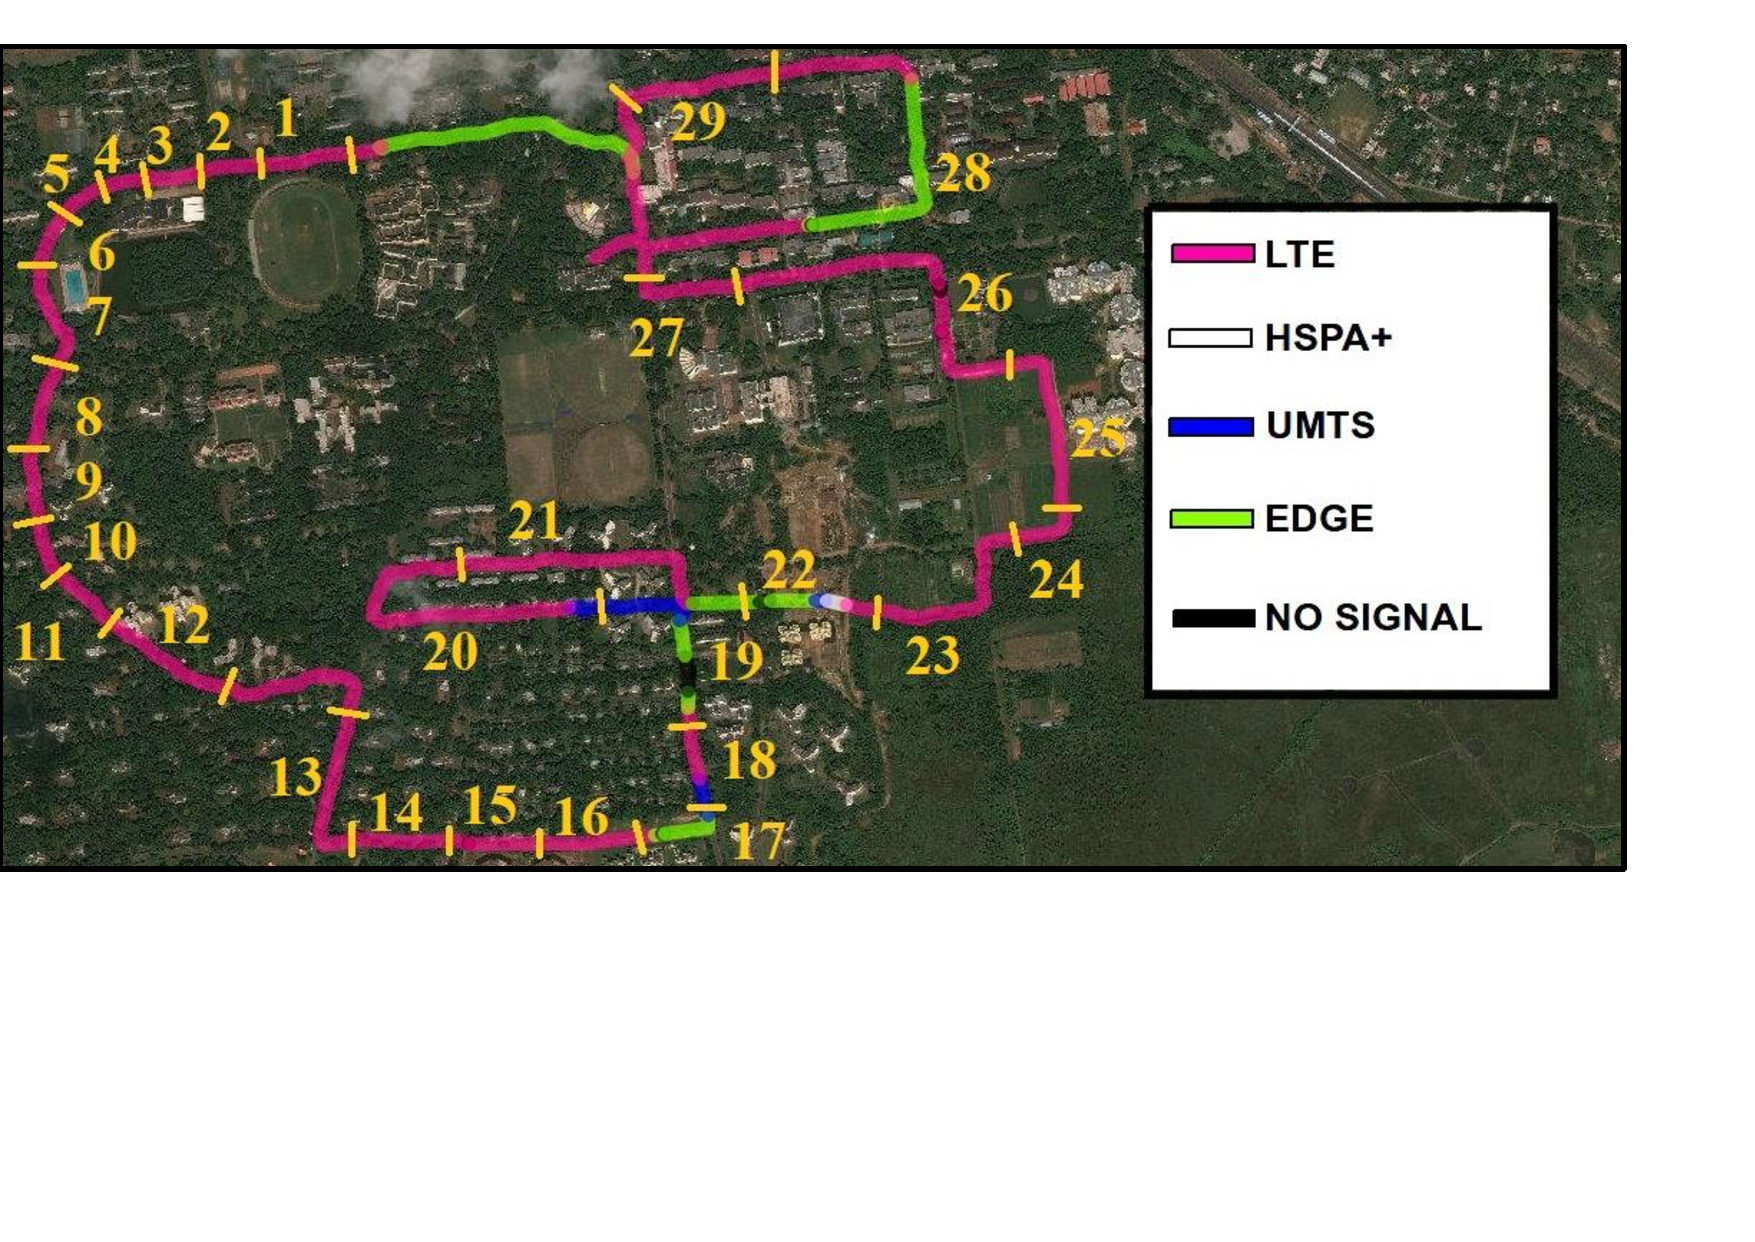
\includegraphics[width = 0.7\linewidth,trim={0cm 6cm 2cm 1cm}]{figures/traj.pdf}
		}\\
		\vspace{+5mm}
		\subfloat[\label{fig:chap03s3:pcap_RSSI}Packet trace of a 360p Youtube video download with the temporal variation in the \ac{RSSI} during the download]{
			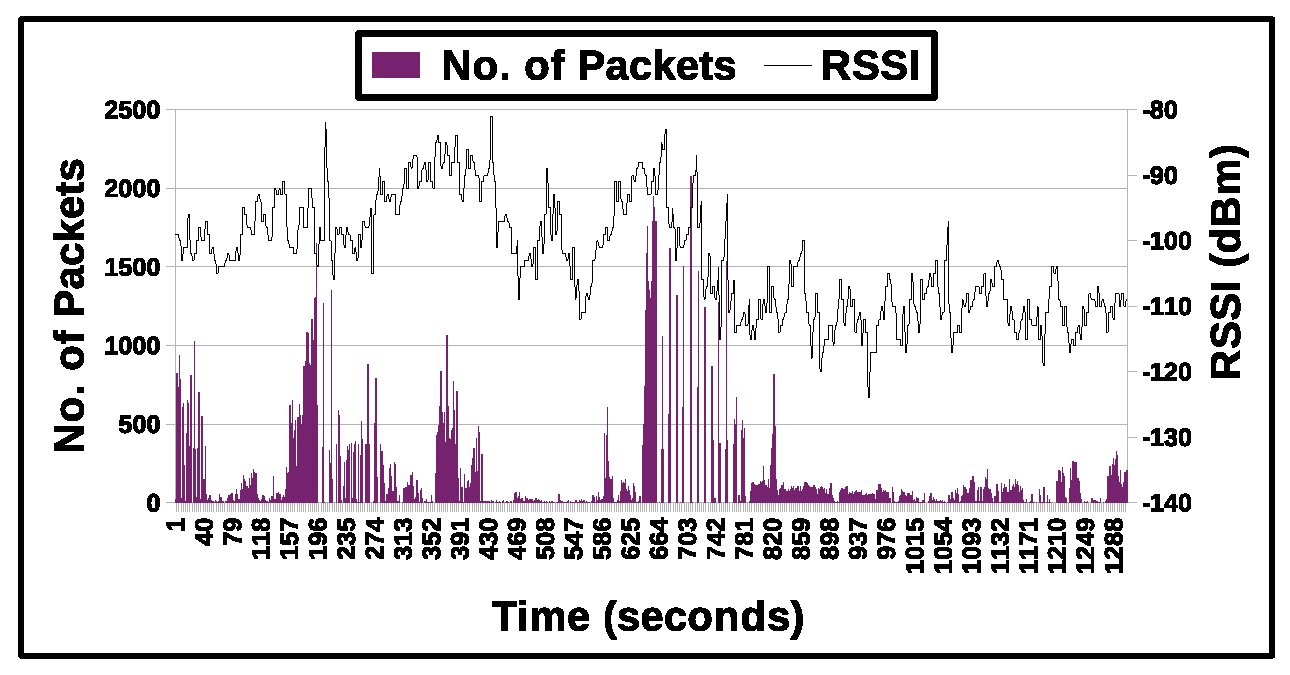
\includegraphics[width=0.7\linewidth,trim={0cm 0cm 0cm 1cm}]{figures/video_rssi_thrpt.eps}
		}
	\end{center}
	\caption{ Experimental Observations}
\end{figure}

\label{sec:chap03s3:EnDASHPilot}
\begin{figure}[!h]
	\captionsetup[subfigure]{width=0.49\linewidth}
	\begin{center}
		\subfloat[\label{fig:chap03s3:setup}The Experimental Setup inside a slow moving electric vehicle]{
			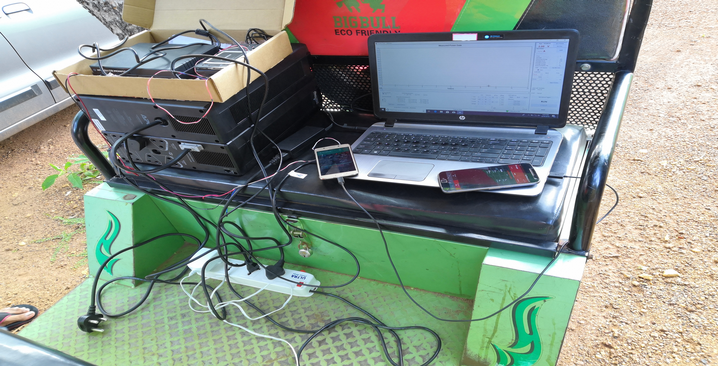
\includegraphics[width=0.49\linewidth]{figures/setup.png}
		}
		\subfloat[\label{fig:chap03s3:thptHO}Sorted throughput of the twenty-nine stretches of \fig{\ref{fig:chap03s3:technology_with_traj}} and its corresponding variations with RSSI, Vertical and Horizontal Handovers]{
			\fbox{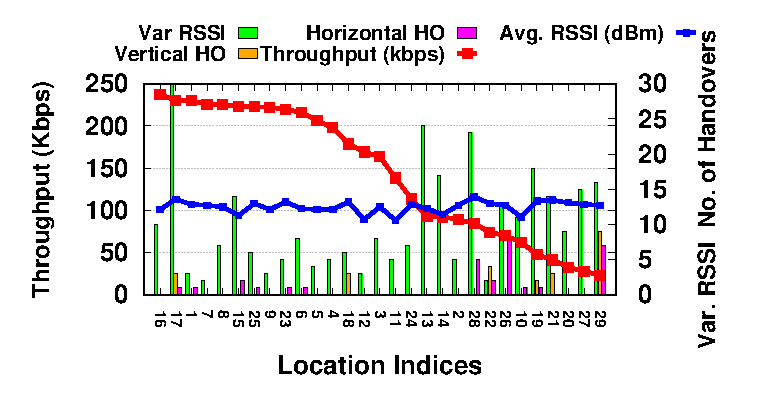
\includegraphics[width=0.49\linewidth]{new_results/pilot/location_throughput}}
		}\\
		\subfloat[\label{fig:chap03s3:powerHO}Variations of Power Consumption with RSSI, and Vertical and Horizontal Handovers over the user's trajectory shown in \fig{\ref{fig:chap03s3:technology_with_traj}}]{
			\fbox{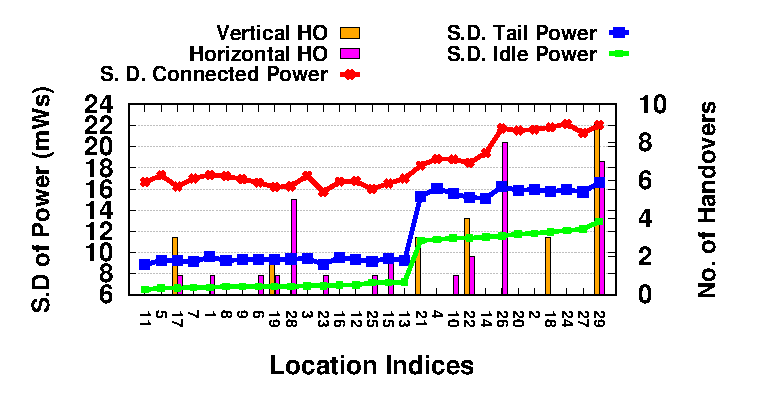
\includegraphics[width=0.49\linewidth]{new_results/pilot/location_power}}
		}
	\end{center}
	\caption{Experimental setup and Throughput and Power consumption variations of a user under mobility; Phone: Moto G5, Service Provider: Airtel}
\end{figure}

%\blue{
%To setup the context, we
%}

%To design an energy efficient video streaming algorithm, which tunes playback buffer length with cellular network throughput, we need a detailed comprehension of the complex relationships between radio related parameters, such as signal strength, vertical and horizontal handovers, speed, etc., on one hand, and throughput and energy consumption on the other hand. To develop this understanding, we have carried out an extensive measurement based study as discussed next.
\subsection{Experimental Set-up}
\subsubsection{Hardware Setup}
For power consumption and energy profiling, we have selected medium budget VoLTE enabled smartphones -  Moto G5  (\$149) and Micromax Canvas Infinity (\$87). Table~\ref{tab:chap03s3:handset_details} outlines their configuration details. We record the power consumption of the phones using Monsoon Solutions High Voltage Power Monitor (HVPM) \cite{HVPM, Yang2018,Geng2015} (Fig.~\ref{fig:chap03s3:setup}) in both stationary and mobile conditions, when connected to three leading mobile internet service providers, Airtel, Reliance JIO, and Vodafone. The \ac{HVPM} records the power at a frequency of 5000 Hz. We have collected power consumption data in three different cities (Kolkata, Kharagpur, Guwahati).
\begin{table}[!h]
    \scriptsize
    \centering
      \caption{Details of the mobile handsets used}
    \begin{tabular}{|p{0.6cm}||p{3.4cm}|p{3.4cm}|}
    \hline
         \textbf{}  & \textbf{Moto G5 (Price: US\$ ~149)} & \textbf{Micromax Canvas Infinity (Price US\$ ~87)}\\
          \hline \hline 
         N/W Tech. & GSM/ HSPA/ LTE &  GSM/ HSPA/ LTE\\ \hline
         N/W Speed & HSPA 42.2/5.76 Mbps, LTE Cat4 150/50 Mbps & HSPA 42.2/5.76 Mbps, LTE Cat4 150/50 Mbps\\ \hline
         OS & Android 7.0 (Nougat) & Android 7.1.2 (Nougat) \\ \hline
         Chipset & Qualcomm MSM8937 Snapdragon 430 (28 nm) & Qualcomm MSM8917 Snapdragon 425 (28 nm)\\ \hline
         CPU & Octa-core 1.4 GHz Cortex-A53 & Quad-core 1.4 GHz Cortex-A53\\ \hline
         GPU & Adreno 505 & Adreno 308\\ \hline
    \end{tabular}
    \label{tab:chap03s3:handset_details}
\end{table}
\indent Besides power consumption, we have also collected extensive data on the received throughput of mobile phones in public buses, cars, and while walking across five cities of India (Kharagpur, Kolkata, Guwahati, Bengaluru, Malda). This dataset also includes data collected while travelling on highways. We have used workloads of 6Mb, 100Mb, 1GB file download, as well as of video streaming using Netflix, Hotstar, SonyLiv and Amazon Prime. This has allowed a detailed energy profiling of the smartphones. The entire corpus of collected data traces amounts to more than 50GB and has been collected over a period of eleven months. 
\subsubsection{Software Setup and Outcome}
\indent In this section, we outline the software setup. We have considered two primary workloads- (a) file download, and (b) video streaming. \\
\begin{figure}[h]
    \centering
    \fbox{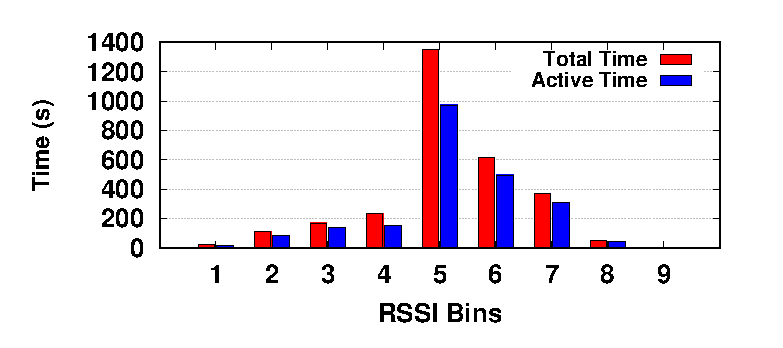
\includegraphics[width=0.7\textwidth]{new_results/pilot/rssi_bin_time}}
    \caption{Total time spent in each \ac{RSSI} bin and the active time in each bin}
    \label{fig:chap03s3:vid_time}
\end{figure}
\begin{figure}[h]
    \centering
    \fbox{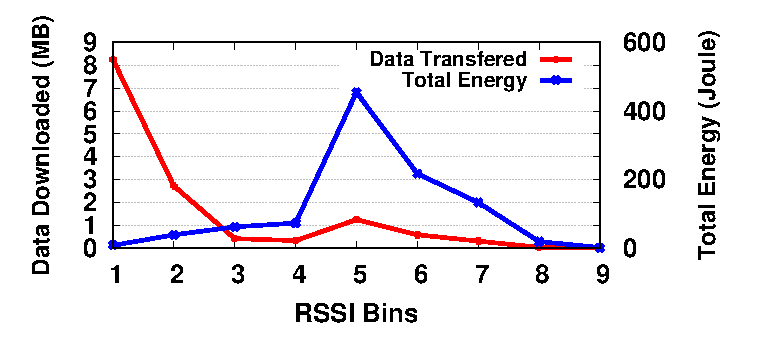
\includegraphics[width=0.7\textwidth]{new_results/pilot/rssi_bin_energy}}
    \caption{Amount of data downloaded \& Energy Consumption in \ac{RSSI} Bins}
    \label{fig:chap03s3:vid_thpt}
\end{figure}
% \begin{figure*}[t]%
% \centering
% \subfigure[Packet trace of a 360p Youtube video download with the temporal variation in the \ac{RSSI} during the download]{%
% \label{fig:pcap_RSSI}%
% 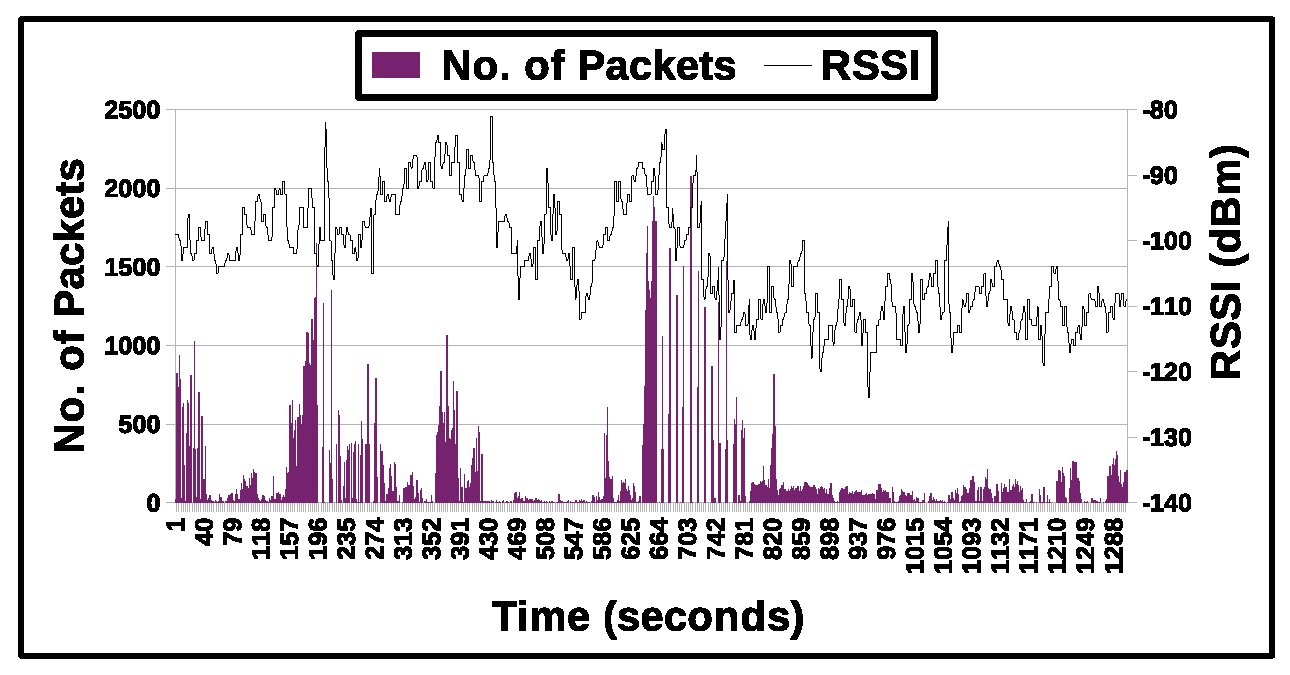
\includegraphics[width=0.31\textwidth]{figures/video_rssi_thrpt.eps}}%
% \hspace{0.1cm}
% \subfigure[Total time spent in each \ac{RSSI} bin and the active time in each bin]{%
% \label{fig:vid_time}%
% 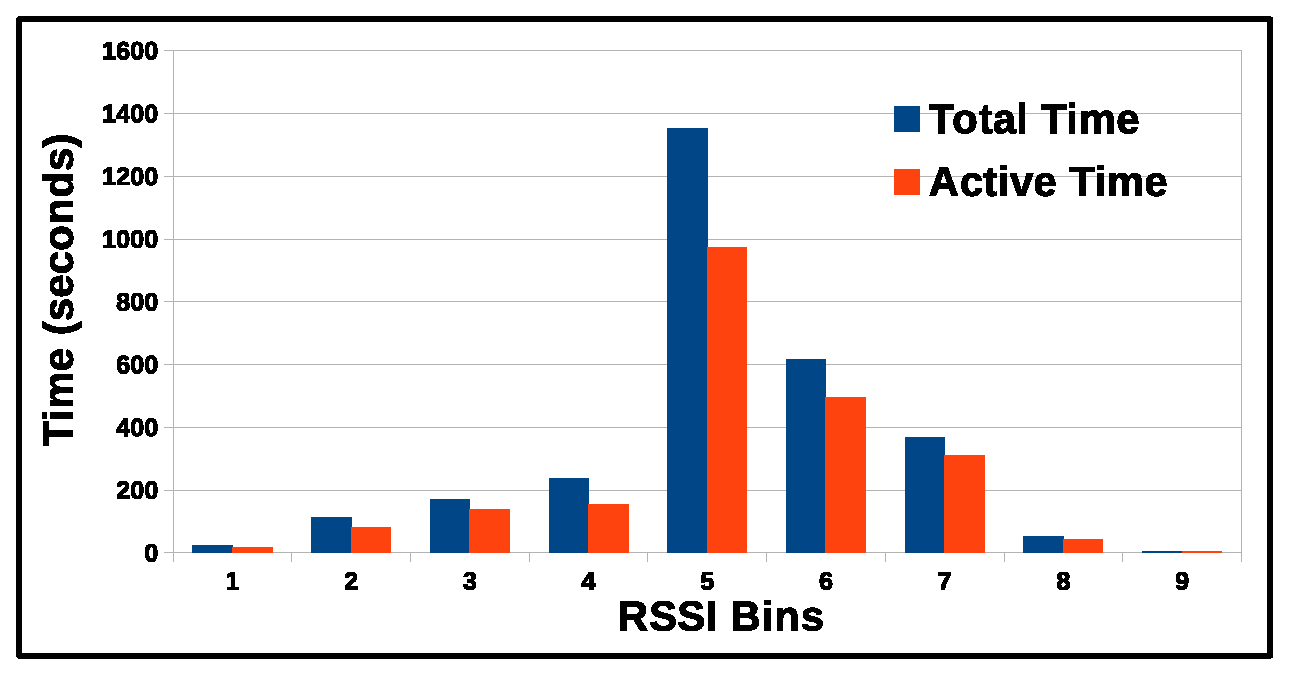
\includegraphics[width=0.31\textwidth]{figures/Video_Time_SNR_bins.eps}}%
% \hspace{0.1cm}
% \subfigure[Amount of data downloaded and Power Consumption in each \ac{RSSI} Bin]{%
% \label{fig:vid_thpt}%
% 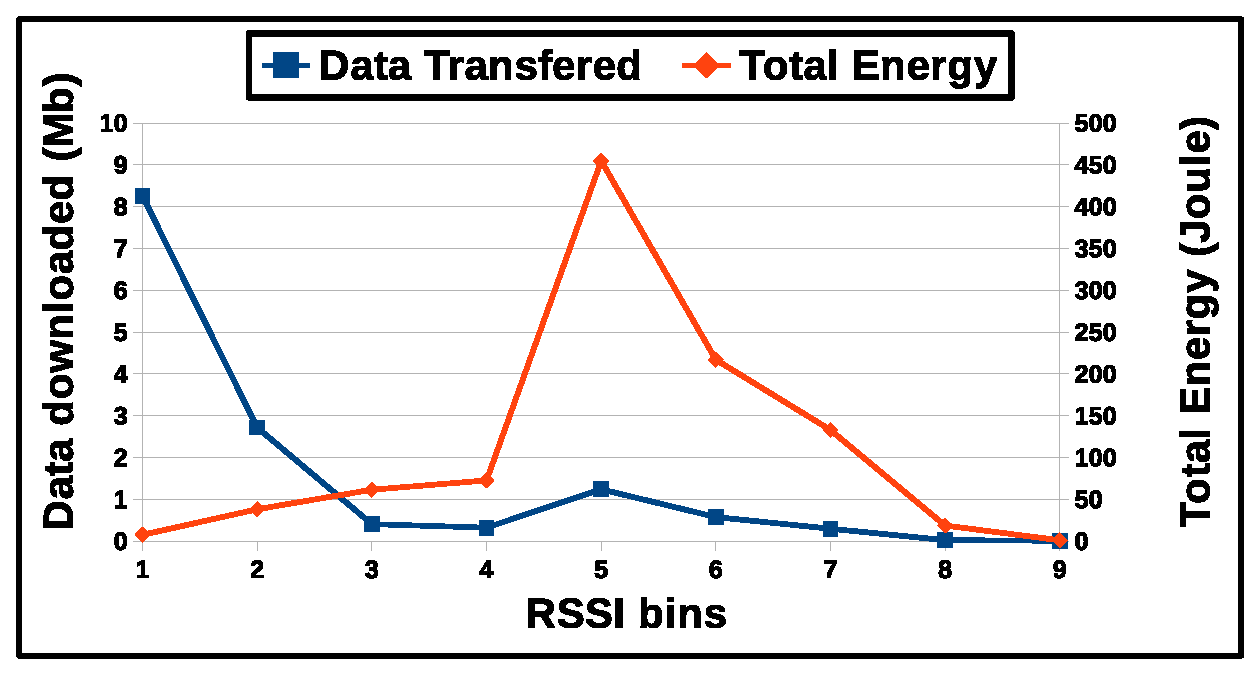
\includegraphics[width=0.31\textwidth]{figures/Video_thpt_power.eps}}%
% \caption{Statistics of YouTube video download to Moto G5 using Airtel mobile internet}\vspace*{-0.5cm}
% \end{figure*}
{\textbf{(a) File Download}} We have used file downloads to profile the power consumption in different RRC states. To enable the download, we have developed  an HTTP client-server program, where the client program runs in the phone and the server  is hosted on an Amazon Web Server (AWS). We have collected traffic traces, radio related information, and location and speed information using \ti{tcpdump}, Network Monitor Lite, and GPS Logger applications, respectively. The collected traffic traces have been analyzed using Wireshark. We have followed \cite{Yang2018} to derive  the RRC state diagram. Accordingly, to measure the \ti{IDLE} state power, we have kept the screen ON, uninstalled all non-default applications, kept all background applications disabled, the WiFi interface turned off, and the mobile network interface switched on but without any active traffic transmission. The corresponding power consumed by the operating system, processor, display, some default background and network-related operations, etc., constitutes the \ti{IDLE} state power.  We have continued measuring the power consumption starting from the \ti{IDLE} state, throughout the file download till the trace came back to the \ti{IDLE} power. Once a file download starts, a jump in power consumption is noted. After the download completes, it drops to an intermediate value during the tail time before returning to the \ti{IDLE} state \cite{Yang2018}. To derive the RRC states, we have downloaded files of different lengths several times using different phones and service providers  in the different cities in stationary condition. The power consumption and dwell time of each RRC state has been found to be different for different phones, service providers as well as c


\indent  Since the corpus of collected data traces is large, we use one such trace to discuss some interesting observations due to space limitations. We call this a `\ti{typical}' trace which was obtained on a single day when downloading 6MB files to the Moto G5 phone while moving around the IIT Kharagpur campus in a hybrid electric vehicle. The set-up is shown in Fig.~\ref{fig:chap03s3:setup}. As Airtel has significantly fluctuating signal quality inside the campus, we chose it as our service provider.  For this `\ti{typical}' trace we had downloaded a 6Mb file to our phone several times. During each download session, the vehicle had moved over a different stretch of the trajectory inside the IIT Kharagpur campus.  Of all the downloads, the twenty-nine stretches  shown in \fig{\ref{fig:chap03s3:technology_with_traj}} could be identified as valid. The sorted throughput over all the twenty-nine stretches of  \fig{\ref{fig:chap03s3:technology_with_traj}} is plotted in descending order in \fig{\ref{fig:chap03s3:thptHO}}. The $x$-axis represents the location indices corresponding to the sorted throughput. The mean and variance of the \ac{RSSI} and also the horizontal and vertical handovers in each of these stretches is shown in \fig{\ref{fig:chap03s3:thptHO}}.  It is observed that the throughput is affected more negatively by handovers than \ac{RSSI} fluctuations. For example, the average and the variance of \ac{RSSI} is nearly the same  in location stretches-\textbf{29} and \textbf{15}. However, stretch \textbf{29} has a lower throughput due to handovers. Again, vertical handovers between network technologies  are found to have a more negative impact on throughput than horizontal ones, as seen in location stretches {\bf 22}  and {\bf 4}.  The effect of handovers on the variation of \ti{CONNECTED}, \ti{TAIL} and \ti{IDLE} state power is shown in Fig.~\ref{fig:chap03s3:powerHO}. It is seen that stretches that witness handovers have a higher variance in  power consumption than no handover stretches. This is because, during handovers, there is a high amount of control information exchange which leads to the rise in \ti{IDLE} power. Moreover, handovers are associated with lower throughput which increases the \ti{CONNECTED} power. Fluctuating signal quality during handover increases the retransmissions and hence the TAIL state power variations.


$\mathrm{\mathbf{\underline{Takeaway:1}}}:$ \textit{The wireless network condition is best quantified by throughput which depends  significantly on phenomena such as handovers and not  on received signal quality alone.}\\
{\textbf{(b)Video Streaming}}\label{sec:chap03s3:vstreaming}
To understand how throughput fluctuation affects video streaming, 
we show the packet trace of a YouTube video of length 20 minutes captured when moving along the trajectory of \fig{\ref{fig:chap03s3:technology_with_traj}}.  Although we learn from the previous section that it is best to quantify the network condition using throughput, in this section we analyze the video download using \ac{RSSI} only. This is because it is difficult to capture the actual network throughput of a phone while any other application (in this case YouTube) is running.\\
\indent The  captured trace and the \ac{RSSI}  is shown in \fig{\ref{fig:chap03s3:pcap_RSSI}}. It is seen that the application downloads video chunks even at low \acp{RSSI}. To understand this, we have divided the \acp{RSSI} on the secondary $y$-axis of \fig{\ref{fig:chap03s3:pcap_RSSI}} into nine bins each of width five, starting from -81 dBm to -126 dBm. The time the \ac{UE} spends in each of these bins, and the time it remains active is given in \fig{\ref{fig:chap03s3:vid_time}}. It is seen that the percentage of time the \ac{UE} spends in the best \ac{RSSI} bin, i.e. \bin{1} (-85 to -81 dBm) is less than 1\%. In comparison, the highest dwell time   as well as the highest active time is recorded in \bin{5} where the \ac{RSSI} varies between -115 to -111 dBm. If we focus on the energy consumption in these \ac{RSSI} bins, as given in \fig{\ref{fig:chap03s3:vid_thpt}}, it is seen that the highest energy is also consumed by the phone in \ac{RSSI} \bin{5}. Another obvious effect of downloading at low signal strength is the low amount of data downloaded for a longer amount time; with reference to \ac{RSSI} \bin{5} in \fig{\ref{fig:chap03s3:vid_thpt}}.


\indent The rate at which the YouTube playback buffer is filled depends on: a) the bandwidth available, and b) the quality of the video requested by the user. Once the buffer length exceeds a threshold, the download stops and restarts only when the buffer length goes below the threshold. So, if the buffer is full when signal quality improves, then the phone does not download any video packet - a possible explanation for no data download between  430-547 seconds in \fig{ \ref{fig:chap03s3:pcap_RSSI}}.


$\mathrm{\mathbf{\underline{Takeaway:2}}}:$ \textit{The current protocol of  video download attributes a higher weightage to the playback-buffer length than the user's instantaneous received signal strength or throughput, ensuing a significantly high energy consumption.}\\
%\indent The takeaways of the pilot study provide the design criteria for designing the EnDASH system, discussed next. 

\section{Summary}
\label{sec:chap03:summary}
In this chapter, we have performed two different experimental studies to analyze the performance of existing \ac{ABR} algorithms from two different fronts. First, we have analyzed the dependency of \ac{ABR} algorithms on the underlying transport protocols. For this purpose, we experimented through the YouTube streaming system as well as based on an in-house lab-scale setup. Second, from an in-the-wild study, we analyzed the power consumption behavior of \ac{ABR} streaming over smartphones. From the first analysis, we observe that although there is a performance dependency on the underlying protocol stack, we actually need to tune the transport layer protocol setups to complement them with the state-of-the-art streaming mechanisms. However, from the second analysis, we observe that we need to tune the existing \ac{ABR} techniques to make them more energy-efficient. From this front, we move forward in developing an energy-efficient streaming mechanism, as discussed in the next chapter.
\clearemptydoublepage

\chapter[EnDASH]
{\textit{EnDASH} - A Mobility Adapted Energy Efficient ABR Video Streaming for Cellular Networks}
\label{chapter04}
\noindent

\renewcommand{\relpath}[1]{Chapters/04.EnDASH/}
\graphicspath{{Chapters/04.EnDASH/}}

\definecolor{LightBlue}{rgb}{0.67,0.847,0.9}
\definecolor{LightOrange}{rgb}{1,0.84,0.60}
\definecolor{LightGrey}{rgb}{0.9,0.9,0.9}

\newcommand{\secBest}[1]{\cellcolor{LightBlue}{#1}}
\newcommand{\best}[1]{\cellcolor{LightOrange}{#1}}
\newcommand{\todo}[1]{\textcolor{red}{TODO: #1}}
\newcommand{\niloy}[1]{\textcolor{red}{NG: #1}}
\newcommand{\bs}[1]{\textcolor{purple}{#1}}
\newcommand{\new}[1]{\textcolor{blue}{#1}}
\newcommand{\ti}[1]{\textit{#1}}
\newcommand{\mq}[1]{$`{#1}$'}
\newcommand{\fig}[1]{Fig.~#1}
\newcommand{\phone}[1]{$\text{P}_{#1}$}
\newcommand{\network}[1]{$\text{N}_{#1}$}
\newcommand{\location}[1]{\textit{Location}-{#1}}
\newcommand{\bin}[1]{{\textit{bin}}-{#1}}
\newcommand{\prefu}[2]{\mathrm{P_{#1}F_{#2}}}
\newcommand{\bracket}[1]{\left({#1}\right)}
\newcommand{\braces}[1]{\left{{#1}\right}}


\section{\textbf{Introduction}}\label{sec:chap04:intro}
With the pervasive roll out of the \ac{4G} cellular networks, online video streaming in smartphones has become one of the most popular modes of entertainment~\cite{CISCO2019}, especially in many developing countries. The availability of ultra cheap data plans, affordable smartphones, and local language based content on YouTube, Netflix, etc., has led to a record increase in the number of mobile video subscribers as well as their engagement time~\cite{Mobstat_2019}.  Subscribers have  shown an inclination towards watching streaming videos even while travelling, irrespective of the distances travelled. Provisioning the expected \ac{QoE} to video users during travelling requires the reception of a stable connection quality at the \acp{UE}, which often eludes users in developing nations. This is because in these countries service providers often compromise on the network infrastructure to provide low cost internet~\cite{Poor_Inf_2019_2}. \\
\indent Another non-negligible impact of mobility on video streaming in  smartphones is the drainage of battery power.  Video streaming itself is a power hungry application~\cite{Xin2012}. Our experiments show that under mobility, video streaming apps consume even more power (\S\ref{sec:chap04:motivation}). The reason for this can be attributed to the fluctuating connection quality experienced while travelling.  This paper proposes to improve the smartphone battery usage through the design of an energy efficient video streaming algorithm that leverages the fluctuating cellular network throughput to choose optimal bitrates while not compromising on the required \ac{QoE}s. \\
\indent To establish the cellular connectivity scenario, 
we have carried out an extensive measurement-based study for eleven months over five different cities in India, including urban areas as well as while travelling on highways (\S\ref{sec:chap04:motivation}). We have recorded the signal received by  medium budget Moto G5 and Micromax phones, while using the cellular data connection of leading service providers in India, like Airtel, Reliance Jio, and Vodafone.
\begin{figure}[h]
	\captionsetup[subfigure]{width=0.7\linewidth}
	\begin{center}
		\subfloat[\label{fig:chap04:technology_with_traj}Trajectory of a VoLTE-enabled android phone inside an academic campus. Associated network standards (4G, HDPA, UMTS, EDGE) highlighted using different colours)]{
			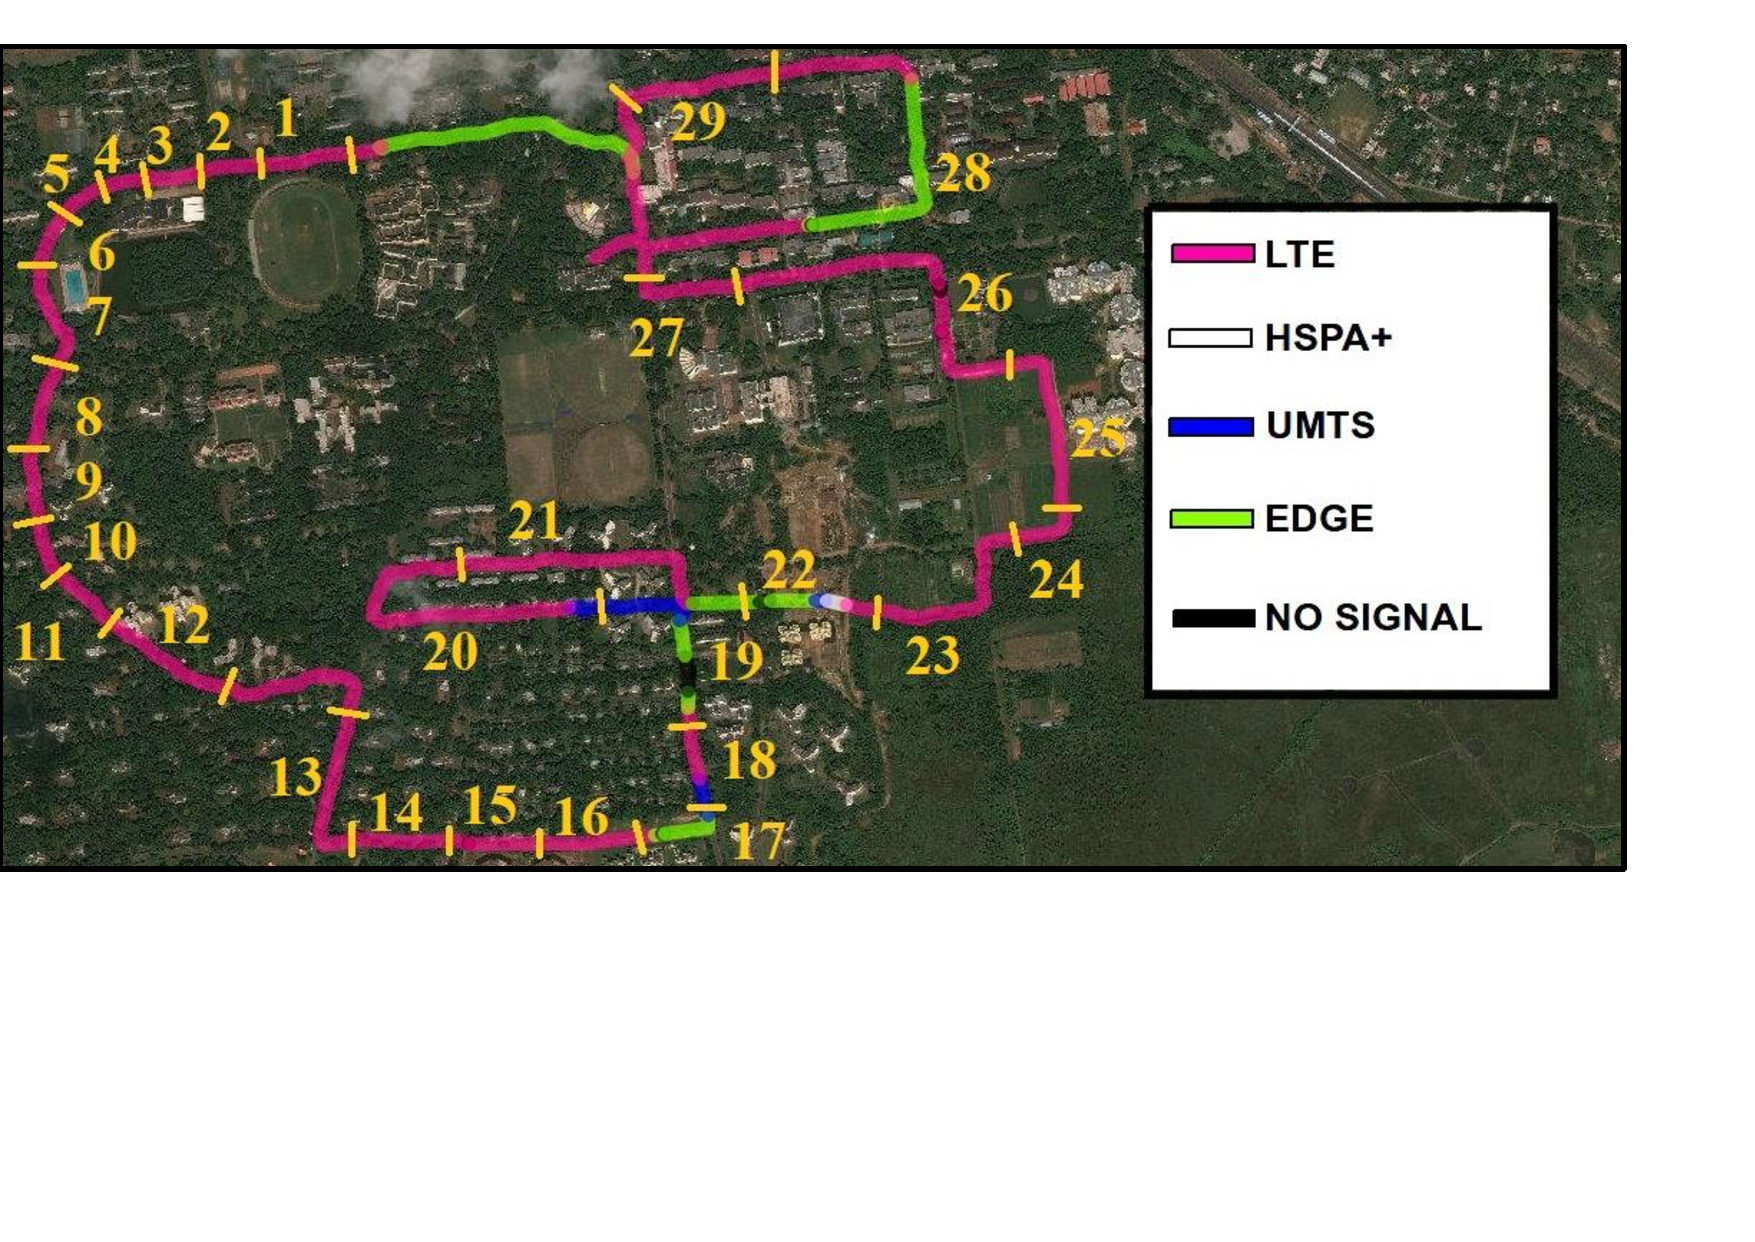
\includegraphics[width = 0.7\linewidth,trim={0cm 6cm 2cm 1cm}]{figures/traj.pdf}
		}\\
	\vspace{+5mm}
		\subfloat[\label{fig:chap04:pcap_RSSI}Packet trace of a 360p Youtube video download with the temporal variation in the \ac{RSSI} during the download]{
			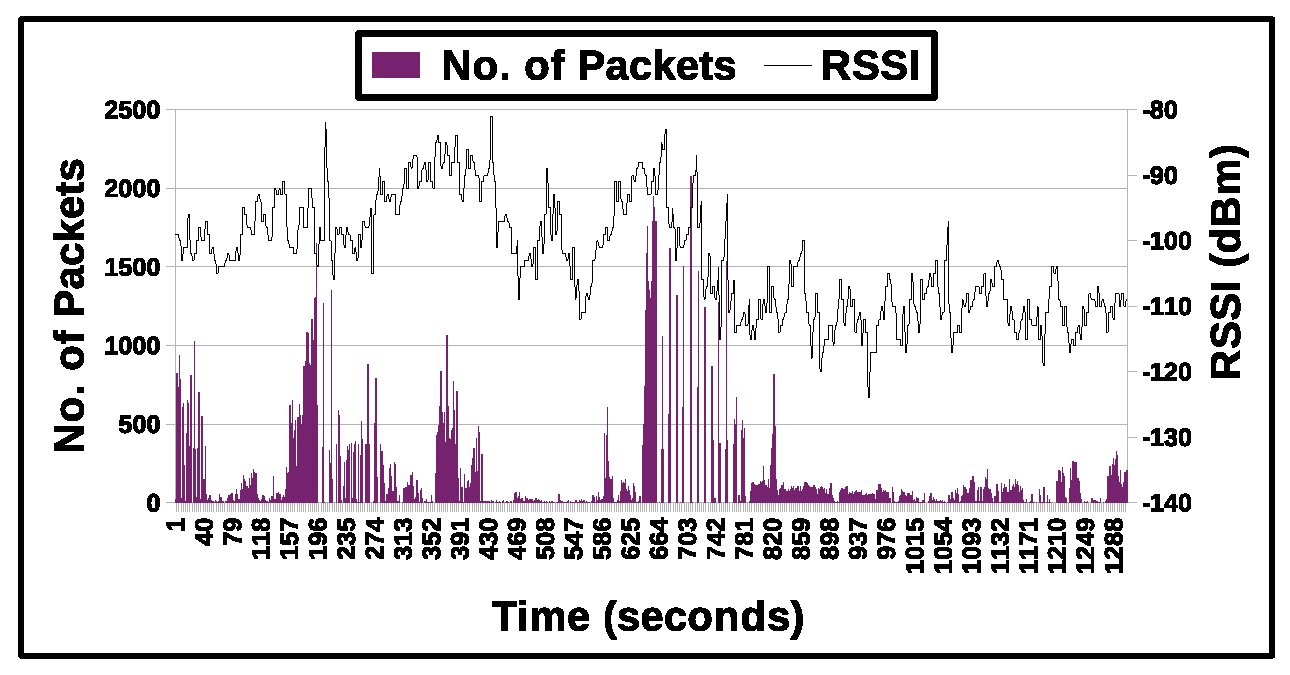
\includegraphics[width=0.7\linewidth,trim={0cm 0cm 0cm 1cm}]{figures/video_rssi_thrpt.eps}
		}
	\end{center}
	\caption{ Experimental Observations}
\end{figure}
%\begin{figure*}[t]%
%\centering
%\subfigure[Trajectory of a VoLTE-enabled android phone inside an academic campus. Associated network standards (4G, HDPA, UMTS, EDGE) highlighted using different colours\vspace*{-0.5cm}]{%
%\label{fig:technology_with_traj}%
%	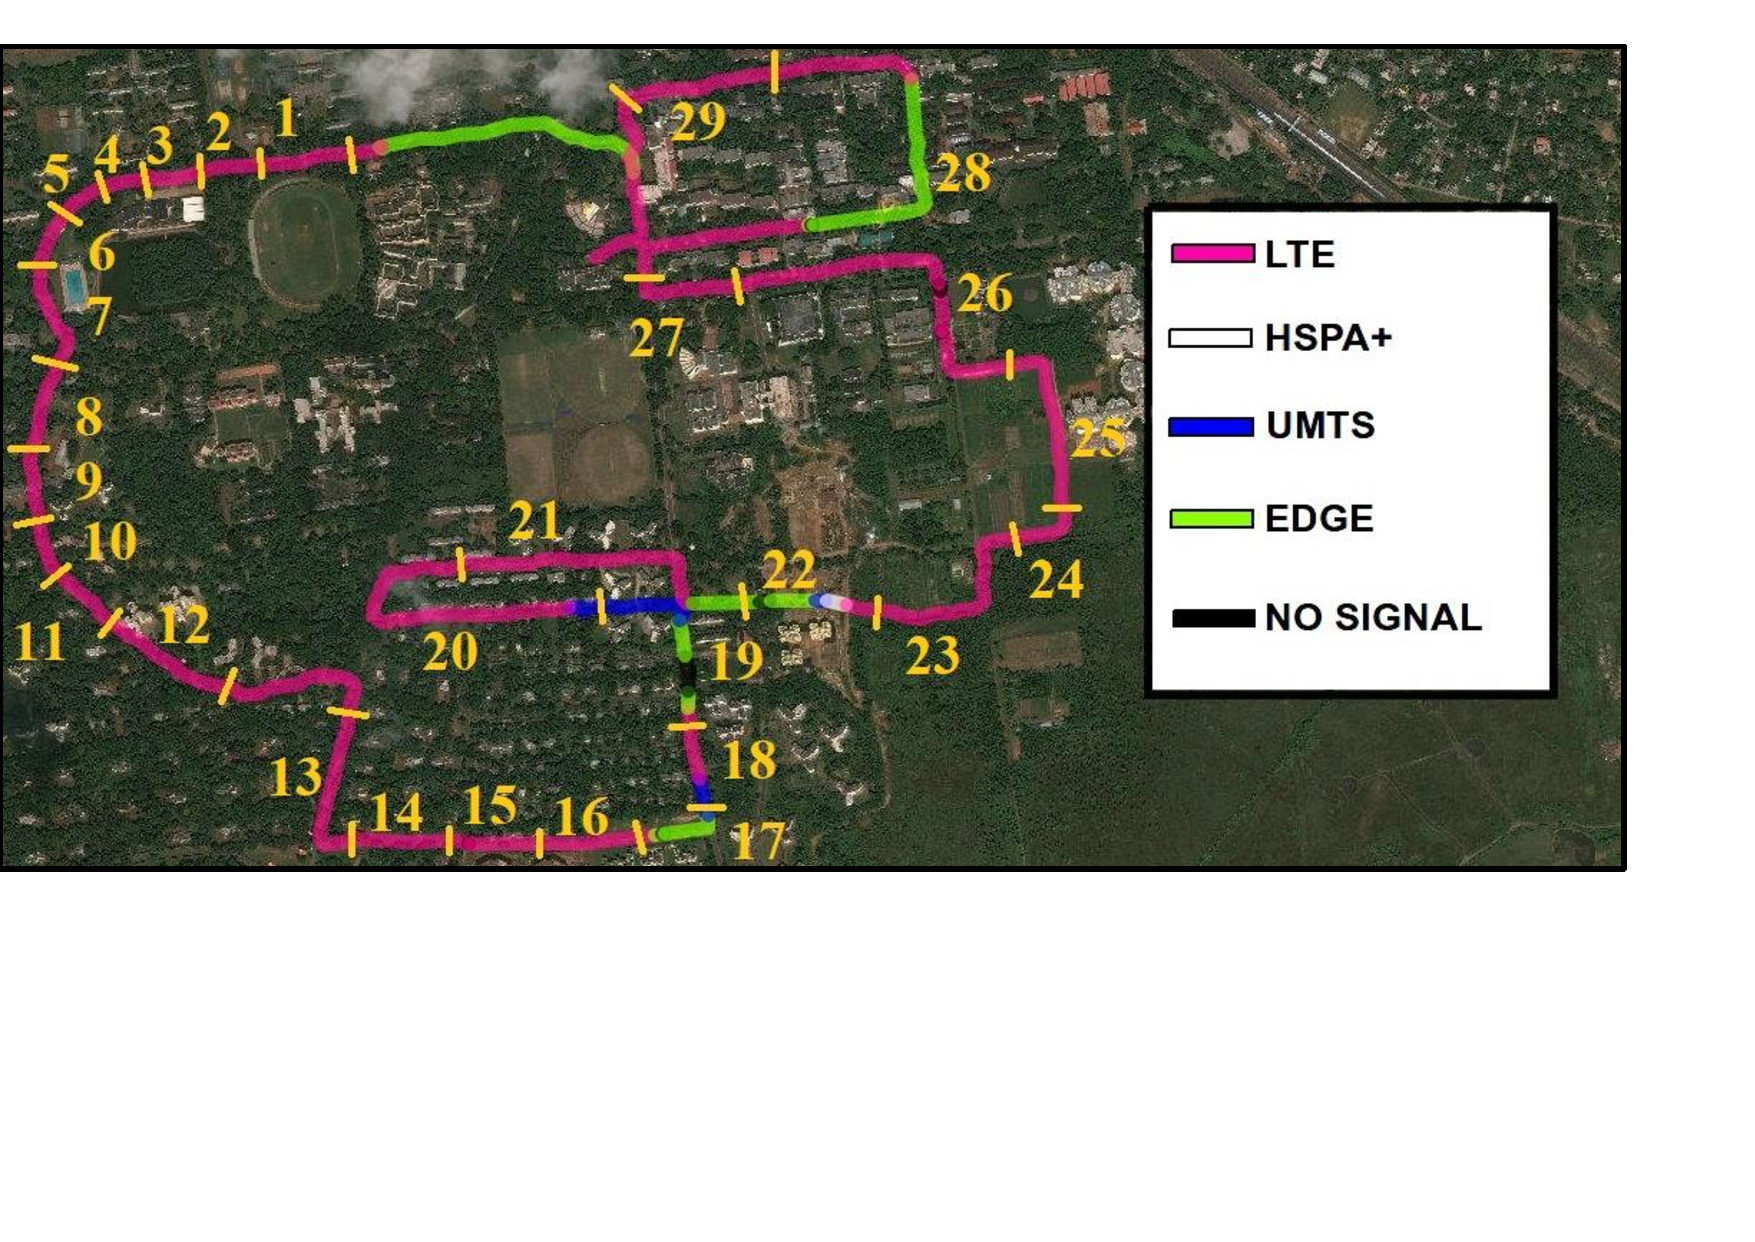
\includegraphics[width = 0.4\textwidth,trim={1cm 7cm 2cm 1cm}]{figures/traj.pdf}}%
%\hspace{2cm}
%\subfigure[Packet trace of a 360p Youtube video download with the temporal variation in the \ac{RSSI} during the download]{%
%\label{fig:pcap_RSSI}%
%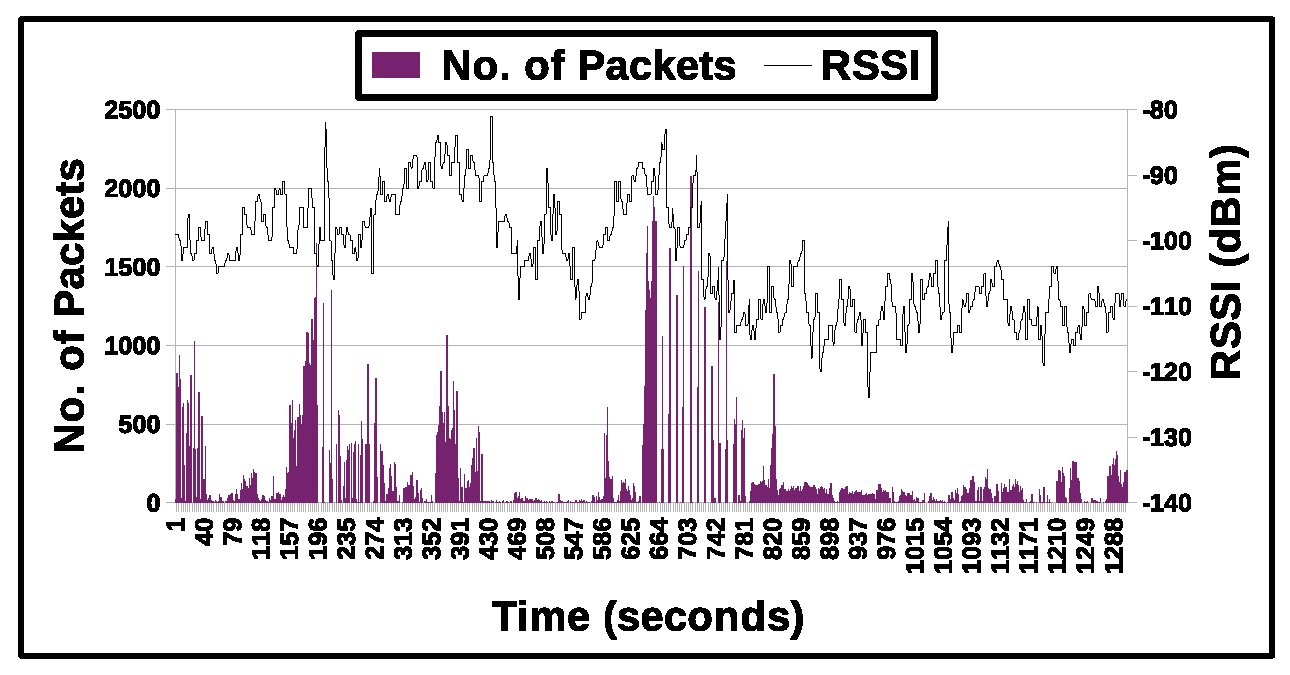
\includegraphics[width=0.4\textwidth,trim={0cm 0cm 0cm 1cm}]{figures/video_rssi_thrpt.eps}}%
%\caption{Experimental Observations}\vspace*{-0.5cm}
%\end{figure*}
A \textit{key finding} of this experiment is shown in Fig.~\ref{fig:chap04:technology_with_traj}, which displays the trajectory of a Moto G5 phone connected to the Airtel network on a single day over the IIT Kharagpur campus area of $8.5$ sq.km. It is seen that even within the small area covered, the phone connects to different generations of cellular technologies, each highlighted in different colours. Two inferences can readily be drawn from Fig. Fig.~\ref{fig:chap04:technology_with_traj}. (i) A service provider does not guarantee a complete \ac{4G} connectivity across the entire coverage region. A \ac{UE} often has to fallback to legacy \ac{3G} or \ac{2G} networks. (ii) Even when connected to \ac{4G}, the signal strength shows random variations. For example, for the experiments conducted, the \ac{RSSI} of \ac{4G} networks fluctuates between $-87$dBm to $-115$dBm. This portrays the typical connectivity scenario in many regions in India.
Another important observation from our experiments, shown in Fig.~\ref{fig:chap04:pcap_RSSI}, is that the volume of data downloaded by video players is not always commensurate with the current network signal strength. Several opportunities to download large chunks of data at high signal strength conditions remain unexploited.


\indent Video streaming applications, including live streaming, predominantly use \ac{DASH} \cite{stockhammer2011dynamic}. In this protocol, the target video is broken into chunks of fixed playback time, and multiple copies of each chunk is stored  at different quality levels, i.e., bitrates.  The client side video player uses \ac{ABR} algorithms~\cite{mao2017neural,Spiteri2016,yin2015control,Raca2019,Akhtar2018}
to decide on the  bitrate at which the next chunk is to be fetched. Existing \ac{DASH} algorithms  primarily take bitrate decisions based on the estimated network throughput or the playback buffer size while attempting to improve user's \ac{QoE}. We, on the other hand, hypothesize that it is possible to significantly lower the energy usage without sacrificing \ac{QoE} if we intelligently utilize the nuances of the cellular network throughput fluctuation during ABR streaming.


\indent To this end, we build an energy
efficient video player {\bf EnDASH} as a wrapper over \ac{DASH} (\S\ref{sec:chap04:sys_overview}).
EnDASH predicts the average cellular network throughput over a finite future time window to take decisions on the opportune fetching of video chunks by dynamically increasing the playback buffer size (\S\ref{sec:chap04:sys_overview}). So, it (i) predicts the the cellular network link throughput from radio related parameters (\S\ref{sec:chap04:thpre}), (ii) then uses the predicted throughput to predict the playback buffer length, and (iii) finally uses the predicted buffer length to choose optimal bitrates for future chunks. Thus, EnDASH consists of three prediction modules, of which the throughput prediction uses random forest learning (step (i)). However, EnDASH works over a smartphone connected to a cellular network which is a randomly varying environment. So, it uses Deep Reinforcement Learning (RL) for the buffer-length prediction mechanism (step (ii)) and bitrate adaptation (step (iii)), which allows EnDASH to exploit the actual performance of previous choices to tune its operation to the current characteristic of the network.  Consequently, EnDASH can start without any apriori knowledge and gradually learn through exploration and exploitation.  The playback buffer length and bitrate decision engines use Deep Neural Networks to map `raw' observations to outputs. These two engines operate using $A3C$ \cite{mao2017neural}, a state-of-the-art actor-critic RL algorithm, and run asynchronously with respect to one another. We train individual prediction modules over a large corpus of collected data traces and evaluate EnDASH using an emulation environment.


\indent Evaluation using our emulation platform shows that in comparison to existing \ac{ABR} algorithms~\cite{mao2017neural,Spiteri2016,yin2015control}, EnDASH significantly improves the energy savings in smartphones (\S\ref{sec:chap04:evaluation}). Energy saved from playing a $2200$ second video using EnDASH can be used to gain an additional $1440$ seconds of video playback time in comparison to the popular Pensieve algorithm~\cite{mao2017neural}. The energy savings, however, comes at the cost of marginally reduced \ac{QoE}.
One of the most salient features of EnDASH, which sets it apart from existing \ac{ABR} algorithms~\cite{mao2017neural,Spiteri2016,Sengupta2018,yin2015control,Raca2019,Akhtar2018,Schulman2010} is that its throughput prediction engine captures the impact of not only the received signal strength but also other network related parameters, such as different technologies and vertical handovers. 
The Mean Absolute Percentage Error (MAPE) of the throughput prediction engine of EnDASH varies from $8\%$ to $13\%$ across different scenarios. The improvement is particularly pronounced in regions having a substantial presence of legacy networks.
The improved throughput prediction assists the EnDASH RL engine to accurately capture the playback buffer evolution, which in turn aids the video segment download in an energy-efficient but QoE favourable manner.\vspace*{-0.2cm}

\section{\textbf{Background and Related Work}}\label{sec:related_work}
% \subsection{Background: DASH system}
%  Adaptive Streaming over HTTP is currently the preferred option for delivering video content.  In \ac{DASH}, a long duration video is broken into chunks of fixed playback time. Successive chunks are aligned in time with each other. Each chunk is stored at \ac{CDN} servers at different bitrates.  A throughput estimator module  estimates the network state, in terms of  the available network throughput, using information on previous chunk downloads. A buffer controller module captures the  video player state using information on streamed video quality and playout-buffer state. Information from both modules are combined by one \ac{ABR} controller to choose an optimal bitrate at which the next chunk is fetched from the \ac{CDN} server. A detailed block diagram of \ac{DASH} can be found in \cite{Sengupta2018} and the references therein.\\
% \indent  State-of-the-art \ac{ABR} algorithms such as MPC \cite{Yin2015}, Pensieve \cite{mao2017neural}, etc. aims to maximize user's \ac{QoE} score, which requires addressing conflicting goals like (a) maximizing overall video quality, (b) minimizing re-buffering time, and (c) increasing smoothness or, i.e., reducing bitrate fluctuations between successive chunks. Due to resource limitations at the client player, complex computations like running a neural network associated with some of these algorithms, e.g. Pensieve,  are run in a stateless \ac{ABR} server. The latency of communication between this server and the \ac{ABR} controller is usually negligible \cite{mao2017neural}. 
%\subsection{RRC state machine of 4G}\label{section:Bckgrd_RRC}
\indent \ac{4G} LTE smartphones are designed to maintain network connectivity using a \ac{RRC} state machine with two states: \textit{CONNECTED} and \textit{IDLE} \cite{Huang2012}. With no active transmission, the \ac{UE} is in the low power \ti{IDLE} state where no radio resource is assigned.  Once a packet arrives, the  \ac{UE} jumps to the high power \ti{CONNECTED} state, in which radio resources are assigned and data transmission takes place.  To reduce the incumbent delay and energy consumption associated with the state promotion, the \ac{UE} waits for a duration called tail time in the \ti{CONNECTED} state before returning to the \ti{IDLE} state even after packet transmission is over. To save energy in the tail period, LTE uses  \ac{DRX} during which the cellular interface periodically monitors the control channel for incoming packets and then goes to sleep ~\cite{Huang2012}. Evidently, if video is downloaded during poor connection quality, then the smartphone will have a longer \ti{CONNECTED} state dwell time resulting in higher energy consumption. Existing \ac{ABR} video streaming algorithms, however, primarily focus on improving \ac{QoE} while paying little attention to energy savings.\\
\noindent \textbf{Improving QoE:}
\ac{ABR} video streaming algorithms either choose buffer occupancy~\cite{Huang2014,Spiteri2016}  or both buffer occupancy and current chunk or network throughput~\cite{Yin2015,Jiang2014,Sengupta2018,Xu2015,Mehr2019} to select optimal bitrates for future video chunks. Examples would be BOLA \cite{Spiteri2016} and MPC \cite{Yin2015}, respectively.
%There are two versions of MPC; Fast MPC- an aggressive approach that uses harmonic mean predictor to estimate future chunk throughput and RobustMPC - a more conservative version which accounts for throughput error. 
Pensieve \cite{mao2017neural} uses a deep RL algorithm for optimal bitrate selection to maximize over a \ac{QoE} metric. However, none of these  works focus on saving device energy consumption under mobility conditions in \ac{4G} LTE networks. \\
\indent In this work, we aim to improve video user's energy consumption over cellular networks while not compromising on \ac{QoE} by tuning playback buffer size to network throughput. Hence, the proposed algorithm should use cellular network throughput prediction.
% \niloy{Does this mean at original level, high definition pictures cannot be seen while here high definition pictures can be seen - this somehow have to come in the study.} \cite{Siris2014} uses mobility and throughput prediction to take decisions on prefetching while moving through a \ac{WiFi}-cellular network.
Several works focus on bandwidth prediction for improving the bitrate selection of  ABR streaming algorithms~\cite{Bentaleb2019,Raca2019,Raca2018_2,yue2018linkforecast}. Some of these works also focus on predicting cellular network throughput~\cite{Raca2019,yue2018linkforecast,Raca2017,Raca2018_2,Raca2018_3,Samba2017, Ghasemi2018}. However, unlike our EnDASH algorithm, none of the works consider the unique situation of co-existence of different technologies and frequent handover from one technology to another for throughput prediction.\\ %In this work, we aim towards using the predicted cellular network throughput to improve energy consumption of \acp{UE}.\\
\noindent\textbf{Reducing Energy Consumption:} Several works in literature investigate energy consumption reduction of mobile phones independently of QoE or ABR streaming algorithms. The BarTendr algorithm in \cite{Schulman2010}  tunes the download sessions in 3G networks to the network conditions for saving energy. However, it quantifies the network condition using received signal strength only while giving no weightage to handovers or associated technologies. GreenTube in \cite{Xin2012} proposes to tune cache management to user behaviour and network conditions. A popular method to reduce energy consumption in mobile phones is to optimize the tail energy, which is achieved in ~\cite{Yang2018} by either prefetching or delaying packets. \\
%\cite{GunerArxiv2018} has proposed power optimization by controlling application-layer parameters such as number of parallel transfers per file, and the number of concurrent fie transfers. \\
%\paragraph{\textbf{\ac{QoS} provisioning for video traffic}} 
% Application layer protocols which prefetch and store video chunks so that the  video quality remains unaffected during poor network conditions are  proposed in \cite{Sengupta2018,Xu2015,Siris2014}. 
\indent To tune packet downloads to network conditions so as to save energy requires a detailed energy profiling of the phones and service providers. This can be obtained through detailed measurement studies as in \cite{Huang2012}. While~\cite{Zhang2018M,Zhang2016,Zhang2016DASH,Khokar2019} focus on the measurement of power consumption of video traffic over HTTP in \ac{4G} networks, the effect of  mobility on signal strength  in \ac{4G} networks is presented briefly. In~\cite{Huang2012, Deng2018} are presented  measurement studies on mobility support in \ac{4G} \ac{LTE} networks. However, to the best of our knowledge, there is no comprehensive measurement study on video streaming under mobility in cellular-only networks. Furthermore, an inherent assumption in these papers is the uninterrupted availability of 4G signal. In contrast, the present work focuses on optimization of energy consumption and \ac{QoE} of mobile video users in scenarios where legacy networks are present in addition to 4G, under mobility conditions.

\section{\textbf{Pilot Study}}\label{sec:chap04:motivation}
\begin{figure}[ht]
	\captionsetup[subfigure]{width=0.49\linewidth}
	\begin{center}
		\subfloat[\label{fig:chap04:setup}The Experimental Setup inside a slow moving electric vehicle]{
			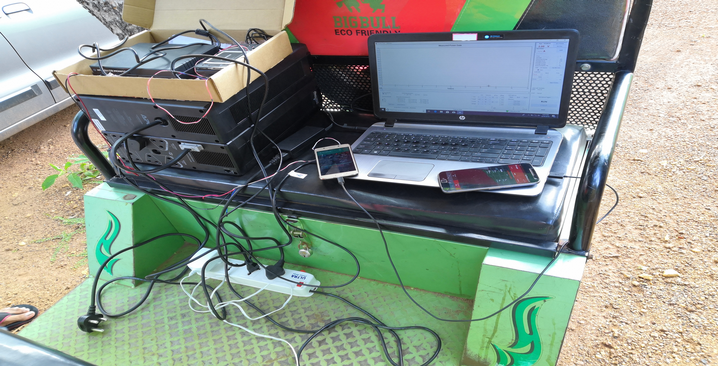
\includegraphics[width=0.49\linewidth]{figures/setup.png}
		}
		\subfloat[\label{fig:chap04:thptHO}Sorted throughput of the twenty-nine stretches of \fig{\ref{fig:chap04:technology_with_traj}} and its corresponding variations with RSSI, Vertical and Horizontal Handovers]{
			\fbox{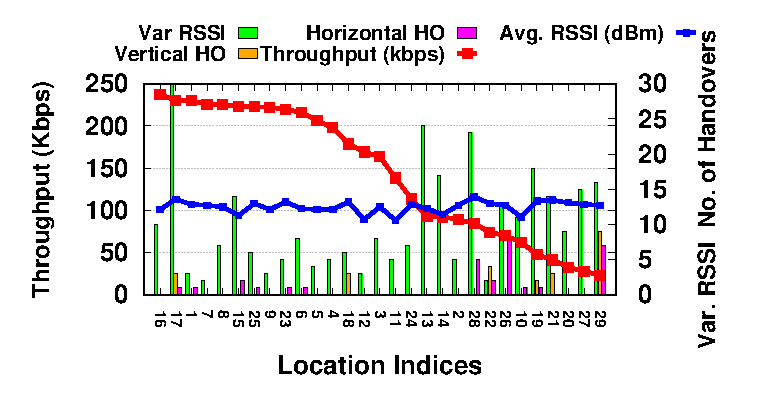
\includegraphics[width=0.49\linewidth]{new_results/pilot/location_throughput}}
		}\\
		\subfloat[\label{fig:chap04:powerHO}Variations of Power Consumption with RSSI, and Vertical and Horizontal Handovers over the user's trajectory shown in \fig{\ref{fig:chap04:technology_with_traj}}]{
			\fbox{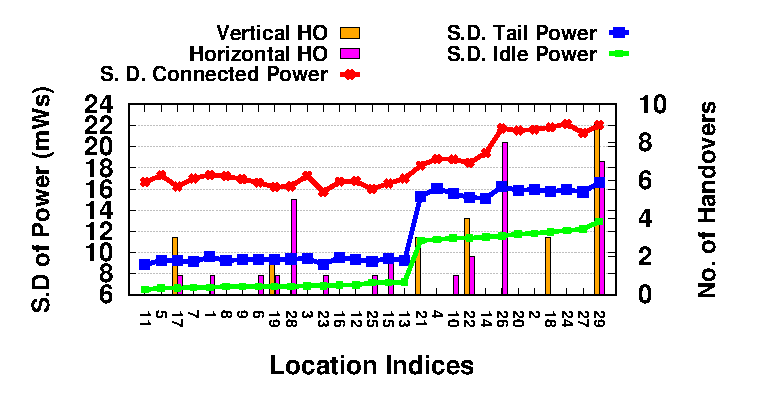
\includegraphics[width=0.49\linewidth]{new_results/pilot/location_power}}
		}
	\end{center}
	\caption{Experimental setup and Throughput and Power consumption variations of a user under mobility; Phone: Moto G5, Service Provider: Airtel}
\end{figure}
%\begin{figure*}[t]%
%\centering
%\subfigure[The Experimental Setup inside a slow moving electric vehicle]{%
% \label{fig:setup}%
% 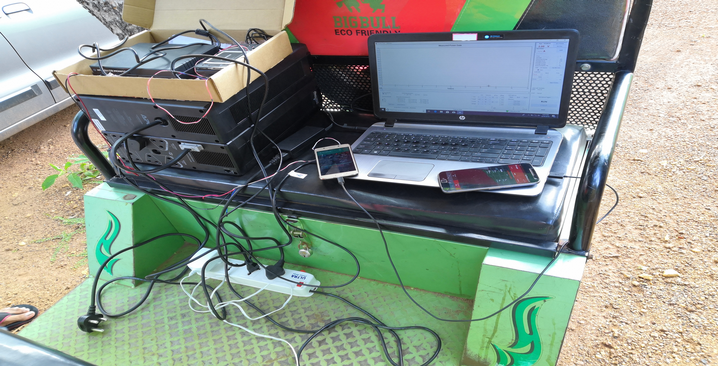
\includegraphics[width=0.31\textwidth]{figures/setup.png}}%
%\hspace{0.1cm}
%\subfigure[Sorted throughput of the twenty-nine stretches of \fig{\ref{fig:technology_with_traj}} and its corresponding variations with RSSI, Vertical and Horizontal Handovers]{%
% \label{fig:thptHO}%
% \fbox{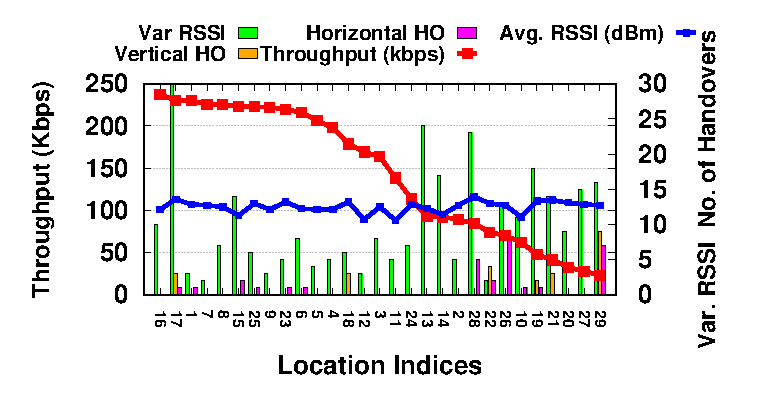
\includegraphics[width=0.31\textwidth]{new_results/pilot/location_throughput}}}%
%\hspace{0.1cm}
%\subfigure[Variations of Power Consumption with RSSI, and Vertical and Horizontal Handovers over the user's trajectory shown in \fig{\ref{fig:technology_with_traj}}]{%
%\label{fig:powerHO}%
%\fbox{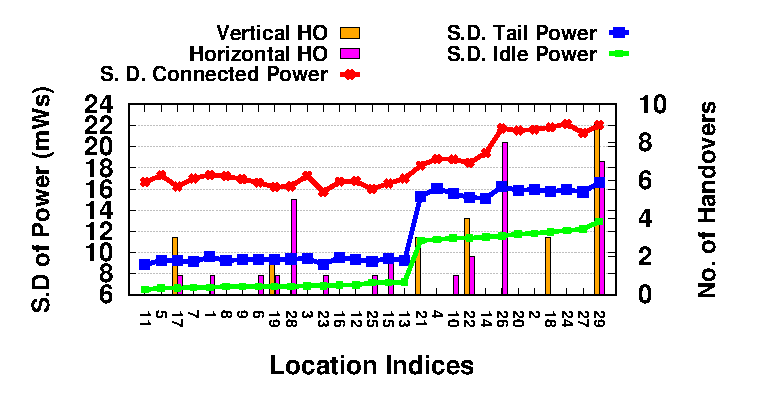
\includegraphics[width=0.31\textwidth]{new_results/pilot/location_power}}}
%\caption{Experimental setup and Throughput and Power consumption variations of a user under mobility; Phone: Moto G5, Service Provider: Airtel}\vspace*{-0.5cm}
%\end{figure*}
%\niloy{The context of the study is also not clear}
To design an energy efficient video streaming algorithm, which tunes playback buffer length with cellular network throughput, we need a detailed comprehension of the complex relationships between radio related parameters, such as signal strength, vertical and horizontal handovers, speed, etc., on one hand, and throughput and energy consumption on the other hand. To develop this understanding, we have carried out an extensive measurement based study as discussed next.
\subsection{Experimental Set-up}
\subsubsection{Hardware Setup}
For power consumption and energy profiling, we have selected medium budget VoLTE enabled smartphones -  Moto G5  (\$149) and Micromax Canvas Infinity (\$87). Table~\ref{tab:chap04:handset_details} outlines their configuration details. We record the power consumption of the phones using Monsoon Solutions High Voltage Power Monitor (HVPM) \cite{HVPM, Yang2018,Geng2015} (Fig.~\ref{fig:chap04:setup}) in both stationary and mobile conditions, when connected to three leading mobile internet service providers, Airtel, Reliance JIO, and Vodafone. The \ac{HVPM} records the power at a frequency of 5000 Hz. We have collected power consumption data in three different cities (Kolkata, Kharagpur, Guwahati).
\begin{table}[!t]
    \scriptsize
    \centering
      \caption{Details of the mobile handsets used}
    \begin{tabular}{|p{0.6cm}||p{3.4cm}|p{3.4cm}|}
    \hline
         \textbf{}  & \textbf{Moto G5 (Price: US\$ ~149)} & \textbf{Micromax Canvas Infinity (Price US\$ ~87)}\\
          \hline \hline 
         N/W Tech. & GSM/ HSPA/ LTE &  GSM/ HSPA/ LTE\\ \hline
         N/W Speed & HSPA 42.2/5.76 Mbps, LTE Cat4 150/50 Mbps & HSPA 42.2/5.76 Mbps, LTE Cat4 150/50 Mbps\\ \hline
         OS & Android 7.0 (Nougat) & Android 7.1.2 (Nougat) \\ \hline
         Chipset & Qualcomm MSM8937 Snapdragon 430 (28 nm) & Qualcomm MSM8917 Snapdragon 425 (28 nm)\\ \hline
         CPU & Octa-core 1.4 GHz Cortex-A53 & Quad-core 1.4 GHz Cortex-A53\\ \hline
         GPU & Adreno 505 & Adreno 308\\ \hline
    \end{tabular}
    \label{tab:chap04:handset_details}
\end{table}
\indent Besides power consumption, we have also collected extensive data on the received throughput of mobile phones in public buses, cars, and while walking across five cities of India (Kharagpur, Kolkata, Guwahati, Bengaluru, Malda). This dataset also includes data collected while travelling on highways. We have used workloads of 6Mb, 100Mb, 1GB file download, as well as of video streaming using Netflix, Hotstar, SonyLiv and Amazon Prime. This has allowed a detailed energy profiling of the smartphones. The entire corpus of collected data traces amounts to more than 50GB and has been collected over a period of eleven months. 
\subsubsection{Software Setup and Outcome}
\indent In this section, we outline the software setup. We have considered two primary workloads- (a) file download, and (b) video streaming. \\
\begin{figure}[h]
    \centering
    \fbox{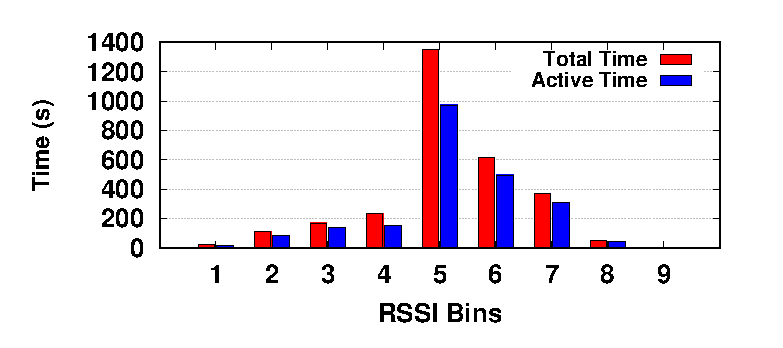
\includegraphics[width=0.7\textwidth]{new_results/pilot/rssi_bin_time}}
    \caption{Total time spent in each \ac{RSSI} bin and the active time in each bin}
    \label{fig:chap04:vid_time}
\end{figure}
\begin{figure}[h]
    \centering
    \fbox{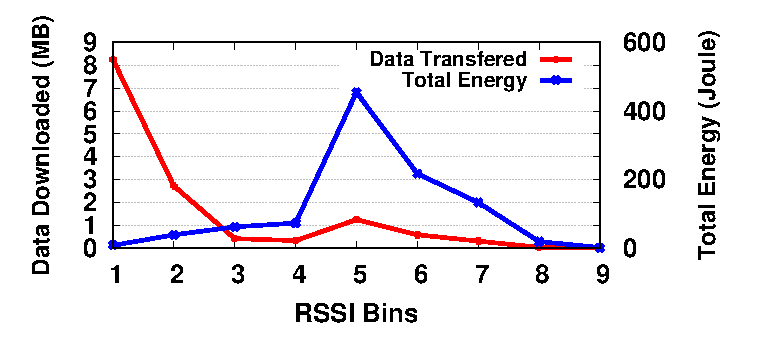
\includegraphics[width=0.7\textwidth]{new_results/pilot/rssi_bin_energy}}
    \caption{Amount of data downloaded \& Energy Consumption in \ac{RSSI} Bins}
    \label{fig:chap04:vid_thpt}
\end{figure}
% \begin{figure*}[t]%
% \centering
% \subfigure[Packet trace of a 360p Youtube video download with the temporal variation in the \ac{RSSI} during the download]{%
% \label{fig:pcap_RSSI}%
% 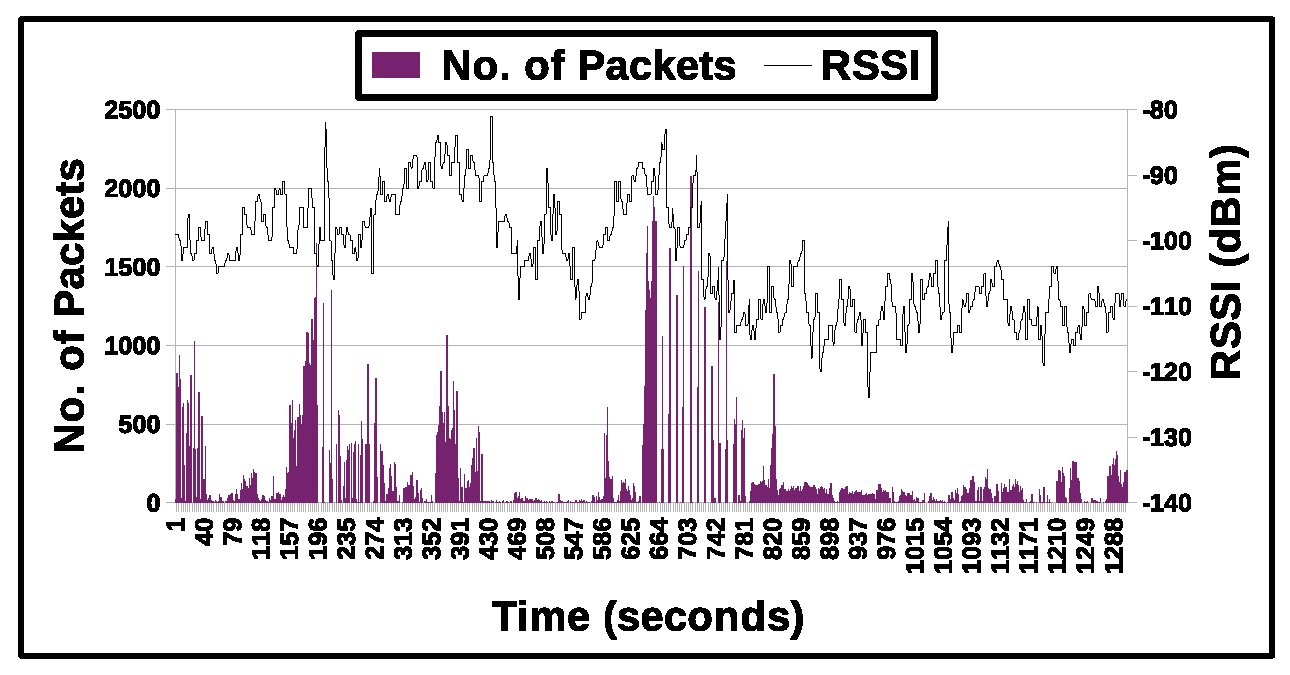
\includegraphics[width=0.31\textwidth]{figures/video_rssi_thrpt.eps}}%
% \hspace{0.1cm}
% \subfigure[Total time spent in each \ac{RSSI} bin and the active time in each bin]{%
% \label{fig:vid_time}%
% 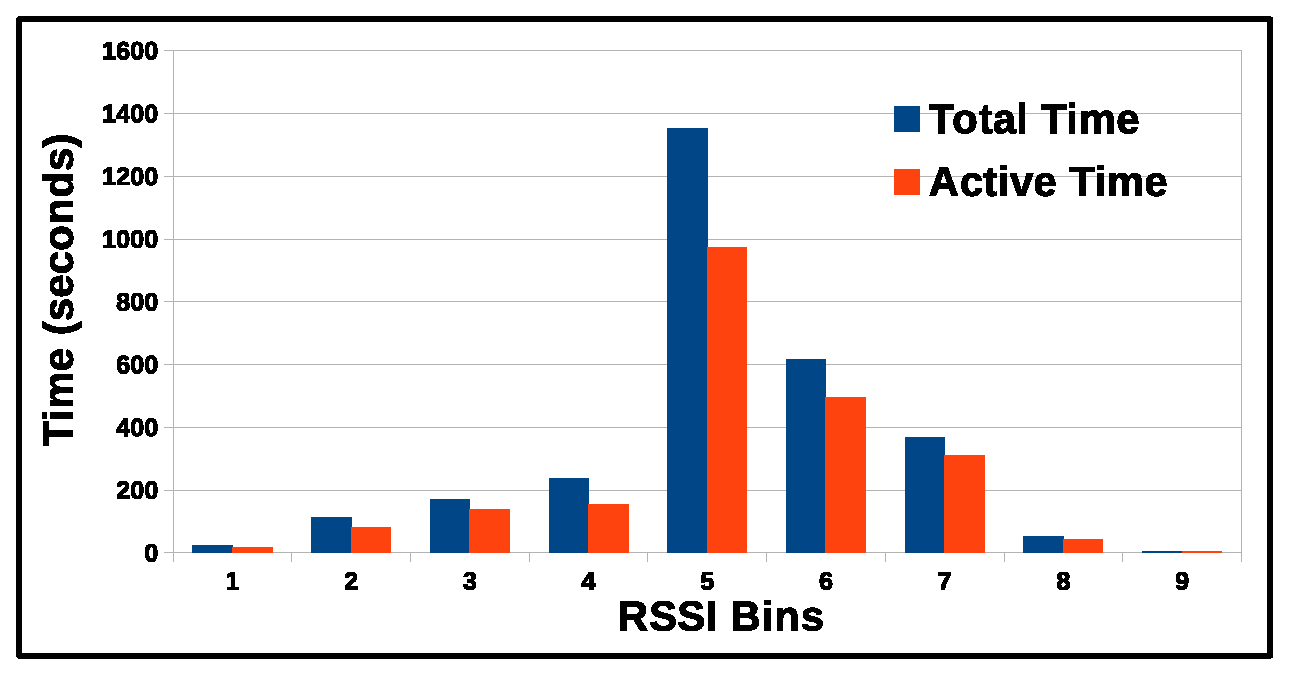
\includegraphics[width=0.31\textwidth]{figures/Video_Time_SNR_bins.eps}}%
% \hspace{0.1cm}
% \subfigure[Amount of data downloaded and Power Consumption in each \ac{RSSI} Bin]{%
% \label{fig:vid_thpt}%
% 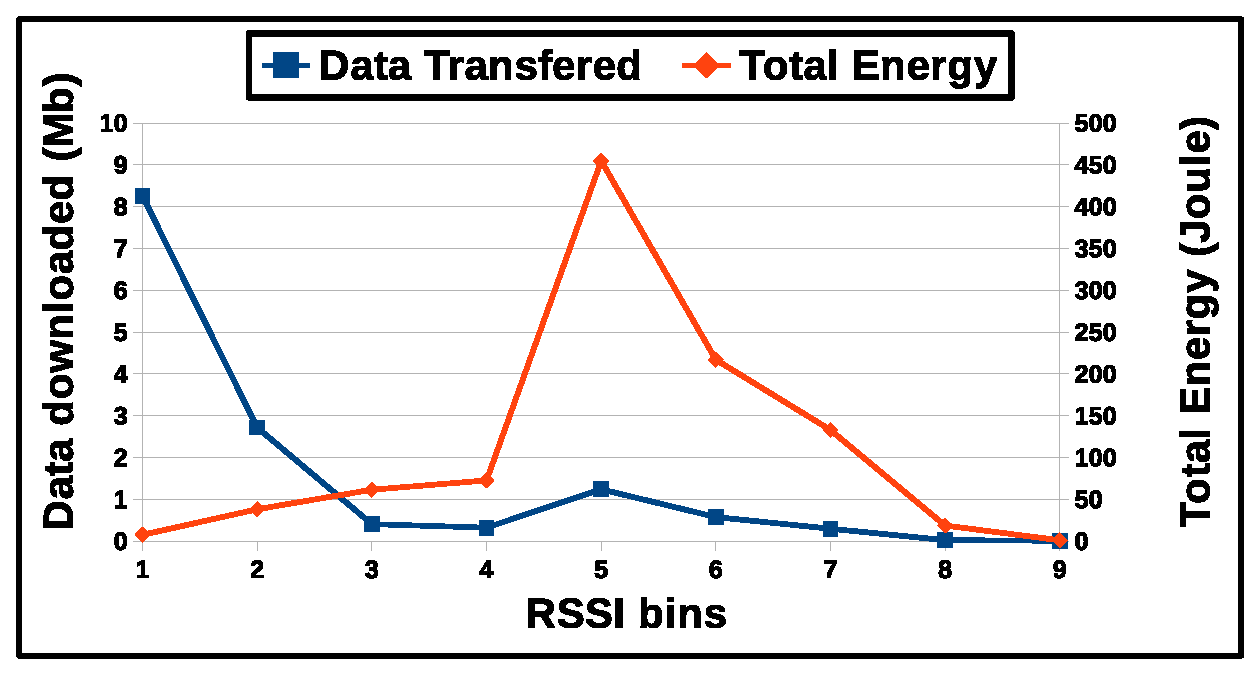
\includegraphics[width=0.31\textwidth]{figures/Video_thpt_power.eps}}%
% \caption{Statistics of YouTube video download to Moto G5 using Airtel mobile internet}\vspace*{-0.5cm}
% \end{figure*}
{\textbf{(a) File Download}} We have used file downloads to profile the power consumption in different RRC states. To enable the download, we have developed  an HTTP client-server program, where the client program runs in the phone and the server  is hosted on an Amazon Web Server (AWS). We have collected traffic traces, radio related information, and location and speed information using \ti{tcpdump}, Network Monitor Lite, and GPS Logger applications, respectively. The collected traffic traces have been analyzed using Wireshark. We have followed \cite{Yang2018} to derive  the RRC state diagram. Accordingly, to measure the \ti{IDLE} state power, we have kept the screen ON, uninstalled all non-default applications, kept all background applications disabled, the WiFi interface turned off, and the mobile network interface switched on but without any active traffic transmission. The corresponding power consumed by the operating system, processor, display, some default background and network-related operations, etc., constitutes the \ti{IDLE} state power.  We have continued measuring the power consumption starting from the \ti{IDLE} state, throughout the file download till the trace came back to the \ti{IDLE} power. Once a file download starts, a jump in power consumption is noted. After the download completes, it drops to an intermediate value during the tail time before returning to the \ti{IDLE} state \cite{Yang2018}. To derive the RRC states, we have downloaded files of different lengths several times using different phones and service providers  in the different cities in stationary condition. The power consumption and dwell time of each RRC state has been found to be different for different phones, service providers as well as c


\indent  Since the corpus of collected data traces is large, we use one such trace to discuss some interesting observations due to space limitations. We call this a `\ti{typical}' trace which was obtained on a single day when downloading 6MB files to the Moto G5 phone while moving around the IIT Kharagpur campus in a hybrid electric vehicle. The set-up is shown in Fig.~\ref{fig:chap04:setup}. As Airtel has significantly fluctuating signal quality inside the campus, we chose it as our service provider.  For this `\ti{typical}' trace we had downloaded a 6Mb file to our phone several times. During each download session, the vehicle had moved over a different stretch of the trajectory inside the IIT Kharagpur campus.  Of all the downloads, the twenty-nine stretches  shown in \fig{\ref{fig:chap04:technology_with_traj}} could be identified as valid. The sorted throughput over all the twenty-nine stretches of  \fig{\ref{fig:chap04:technology_with_traj}} is plotted in descending order in \fig{\ref{fig:chap04:thptHO}}. The $x$-axis represents the location indices corresponding to the sorted throughput. The mean and variance of the \ac{RSSI} and also the horizontal and vertical handovers in each of these stretches is shown in \fig{\ref{fig:chap04:thptHO}}.  It is observed that the throughput is affected more negatively by handovers than \ac{RSSI} fluctuations. For example, the average and the variance of \ac{RSSI} is nearly the same  in location stretches-\textbf{29} and \textbf{15}. However, stretch \textbf{29} has a lower throughput due to handovers. Again, vertical handovers between network technologies  are found to have a more negative impact on throughput than horizontal ones, as seen in location stretches {\bf 22}  and {\bf 4}.  The effect of handovers on the variation of \ti{CONNECTED}, \ti{TAIL} and \ti{IDLE} state power is shown in Fig.~\ref{fig:chap04:powerHO}. It is seen that stretches that witness handovers have a higher variance in  power consumption than no handover stretches. This is because, during handovers, there is a high amount of control information exchange which leads to the rise in \ti{IDLE} power. Moreover, handovers are associated with lower throughput which increases the \ti{CONNECTED} power. Fluctuating signal quality during handover increases the retransmissions and hence the TAIL state power variations.


$\mathrm{\mathbf{\underline{Takeaway:1}}}:$ \textit{The wireless network condition is best quantified by throughput which depends  significantly on phenomena such as handovers and not  on received signal quality alone.}\\
{\textbf{(b)Video Streaming}}\label{sec:chap04:vstreaming}
To understand how throughput fluctuation affects video streaming, 
we show the packet trace of a YouTube video of length 20 minutes captured when moving along the trajectory of \fig{\ref{fig:chap04:technology_with_traj}}.  Although we learn from the previous section that it is best to quantify the network condition using throughput, in this section we analyze the video download using \ac{RSSI} only. This is because it is difficult to capture the actual network throughput of a phone while any other application (in this case YouTube) is running.\\
\indent The  captured trace and the \ac{RSSI}  is shown in \fig{\ref{fig:chap04:pcap_RSSI}}. It is seen that the application downloads video chunks even at low \acp{RSSI}. To understand this, we have divided the \acp{RSSI} on the secondary $y$-axis of \fig{\ref{fig:chap04:pcap_RSSI}} into nine bins each of width five, starting from -81 dBm to -126 dBm. The time the \ac{UE} spends in each of these bins, and the time it remains active is given in \fig{\ref{fig:chap04:vid_time}}. It is seen that the percentage of time the \ac{UE} spends in the best \ac{RSSI} bin, i.e. \bin{1} (-85 to -81 dBm) is less than 1\%. In comparison, the highest dwell time   as well as the highest active time is recorded in \bin{5} where the \ac{RSSI} varies between -115 to -111 dBm. If we focus on the energy consumption in these \ac{RSSI} bins, as given in \fig{\ref{fig:chap04:vid_thpt}}, it is seen that the highest energy is also consumed by the phone in \ac{RSSI} \bin{5}. Another obvious effect of downloading at low signal strength is the low amount of data downloaded for a longer amount time; with reference to \ac{RSSI} \bin{5} in \fig{\ref{fig:chap04:vid_thpt}}.


\indent The rate at which the YouTube playback buffer is filled depends on: a) the bandwidth available, and b) the quality of the video requested by the user. Once the buffer length exceeds a threshold, the download stops and restarts only when the buffer length goes below the threshold. So, if the buffer is full when signal quality improves, then the phone does not download any video packet - a possible explanation for no data download between  430-547 seconds in \fig{ \ref{fig:chap04:pcap_RSSI}}.


$\mathrm{\mathbf{\underline{Takeaway:2}}}:$ \textit{The current protocol of  video download attributes a higher weightage to the playback-buffer length than the user's instantaneous received signal strength or throughput, ensuing a significantly high energy consumption.}\\
\indent The takeaways of the pilot study provide the design criteria for designing the EnDASH system, discussed next. 
\section{EnDASH System}\label{sec:chap04:sys_overview}
The proposed EnDASH system is an energy efficient client video player, working as a wrapper over \ac{DASH}. It predicts the cellular network throughput over a finite future time window to take decisions on the opportune fetching of  video chunks.  EnDASH operates in a time-slotted fashion. So, the entire timeline is divided into discrete time-slots of length \mq{T}.
EnDASH executes the following functions to achieve energy efficient video download: (i) At the beginning of each time slot it uses historical data on radio parameters to predict the cellular network link throughput of the current time slot using a \ac{RFL} engine. (ii) It then uses the predicted throughput to predict the optimal playback-buffer length for the current slot that minimizes energy consumption. For this, EnDASH employs the state-of-the-art \ac{A3C} deep \ac{RL} algorithm.  (iii) Before downloading each video chunk within a time slot, EnDASH runs another A3C based deep \ac{RL} engine to predict the optimal download chunk  bitrate.
EnDASH is, thus, a cascaded system of three engines: (i) throughput prediction, (ii) buffer length decision,  and (iii) bitrate selection as shown in \fig\ref{fig:chap04:EnDASH system}. We next describe these modules.
 \begin{figure}[t]
	\centering
	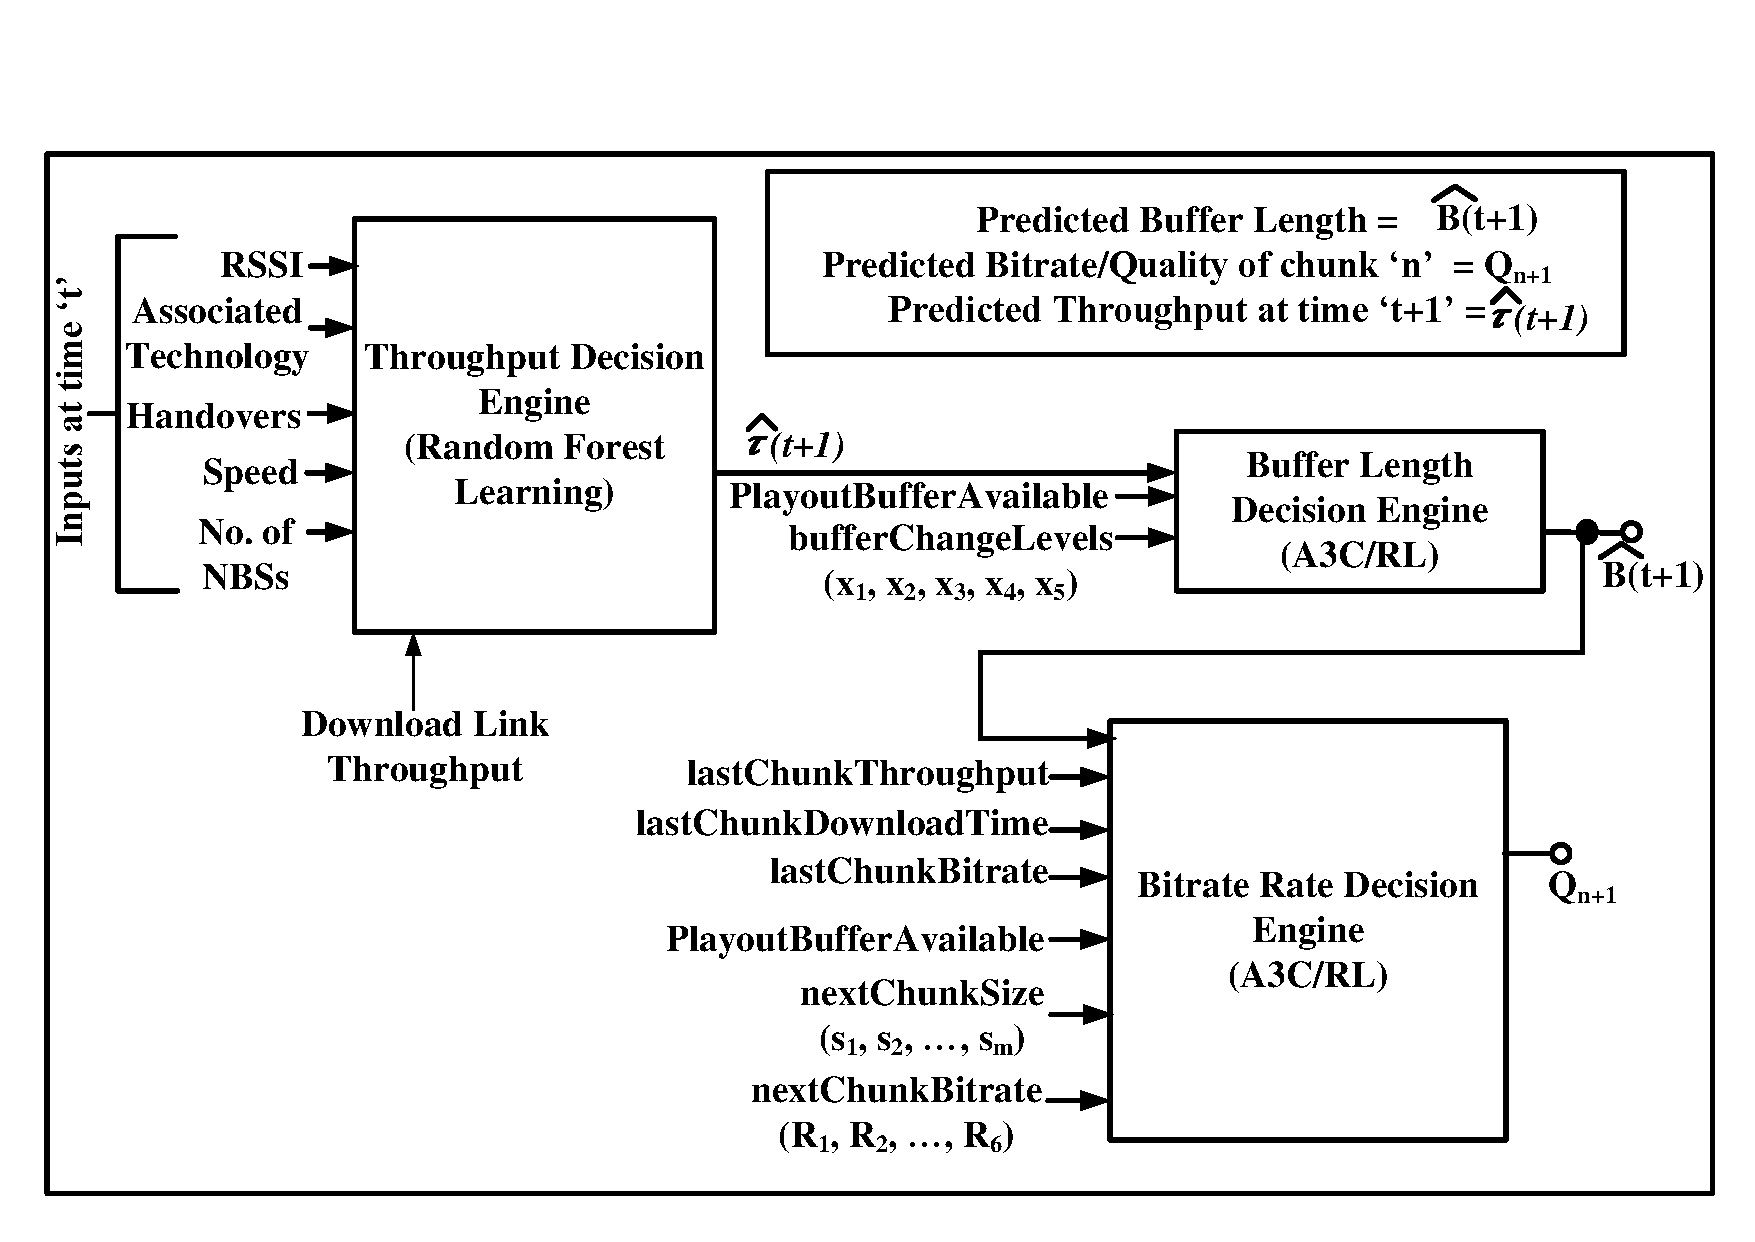
\includegraphics[width = 0.7\textwidth,trim = {1cm 1cm 1cm 1cm}]{figures/EnDASH_system.pdf}
	\caption{Composite Representation of the EnDASH model; a cascaded model where the predicted throughput acts as an input network state to the Actor Critic \acs{RL} based decision engine}
	\label{fig:chap04:EnDASH system}
\end{figure}

\subsection{The Throughput Prediction Engine}\label{sec:chap04:thpre}
EnDASH employs a \ac{RFL} algorithm for cellular network throughput prediction ~\cite{Raca2019}. At the beginning of time slot \mq{t}, it uses the historical information of different radio related parameters in the previous \mq{x} seconds to predict the average throughput~\footnote{Since video rate adaptation algorithms mostly use average throughput, hence for EnDASH, we have predicted the average throughput only \cite{Raca2019}.} that may be experienced by the user during the time slot (of length `T'). We represent this as $\prefu{x}{T}$.
The input features of the throughput prediction engine are: (i) \ti{RSSI}, (b) \ti{technologies used} - LTE (4G), HSPA+ (3.75G), UMTS (3G), EDGE (2G), (c) \ti{number of vertical and horizontal \ti{handovers}}, (d) \ti{speed},  (e) \ti{number and technology of neighbouring \acp{BS}}, (f) \ti{download link throughput} - the download rate is measured at the \ac{UE} in bytes per second. Readings on these features  are obtained from the NetMonitor Lite app with a granularity of one second.

\indent  Each feature can be represented as a distribution,
However, instead of feeding the entire time-series data for each metric, we adopt the summarization technique of \cite{Raca2019}. So, we feed only a few key values that best summarize the data and its corresponding distribution.
For each of the features we obtain the $\mathrm{25^{th}}$, $\mathrm{75^{th}}$, and $\mathrm{90^{th}}$ percentile points, median and mean from its historical data and feed it to the \ac{RFL} algorithm. We train and test this module using 39662 seconds of collected data on received throughput across five Indian cities.

\subsection{The Buffer Length Decision Engine}\label{sec:chap04:buff_length_dec_engine}
\indent The Buffer Length Decision engine also runs at the beginning of each time slot and the playback buffer length is predicted from the predicted network throughput.  However, the relationship between the predicted throughput and the buffer length is not straightforward and is not analytically tractable. So, we employ an A3C \ac{RL} based deep neural network to determine the optimal buffer length.

\indent The components of the \ac{RL} algorithm corresponding to the buffer decision engine are as follows:\\
% \begin{itemize}
\noindent \textbf{(i) Environment}  \ti{E} - video player.\\
\noindent \textbf{(ii) Input state at timeslot `$\kappa$'} $S_\kappa$ =  ($\hat{\tau}_{{\kappa}}$, $B_{av_\kappa}$, ${\mathcal{X}}$), where
  $\hat{\tau}_{{\kappa}}$ is the  average predicted cellular network throughput,
 $B_{av_\kappa}$ is the current playback buffer capacity available in seconds,
$\mathcal{X}$ is the set of possible changes in buffer length. If the current buffer length is $B_{\kappa-1}$, the next buffer length can be predicted to be $\hat{B_\kappa}= B_\kappa+x$ where $x\in\mathcal{X}:=\{-2,-1,0,+1,+2\}$. $x=1$ implies an increase in buffer length by a single chunk.\\
%, each chunk is of eight seconds.\\
\noindent \textbf{(iii) Action} $A_\kappa$ - Decisions on the increase or decrease of buffer length at timeslot $\kappa$. \\
\noindent \textbf{(iv) Reward} - The reward function is defined as a linear weighted function of energy savings with respect to a baseline \ac{ABR} algorithm and the \ac{QoE} score:
    \begin{equation}
    \Xi_{\mathrm{bufflen}} = w_1 \cdot (\left|E_{\mathrm{EnDASH}_\kappa}-E_{\mathrm{old}_\kappa}\right|)+w_2 \cdot QoE
    \end{equation}

\indent The first term in the reward function gives the energy savings with respect to a baseline \ac{ABR} algorithm. In this work, we have chosen BOLA \cite{Spiteri2016} as the baseline since its energy consumption is the lowest among existing algorithms (excluding EnDASH, \S{\ref{sec:chap04:evaluation}}).  $E_{\mathrm{old}_\kappa}$ and $E_{\mathrm{EnDASH}_\kappa}$ represent the energy consumption of BOLA and of EnDASH at time \mq{\kappa}, respectively. The energy consumed while using one particular algorithm is obtained as follows:  the \ac{RRC} states are first identified from the download packet capture of a video trace. Next, the dwell time in each \ac{RRC} state is multiplied by the corresponding power consumption (obtained from the \ac{RRC} state machine) to get the energy quantities. We calculate the energy savings in this manner because the ground truth on energy consumption cannot be obtained.

\indent Second term in the reward function is the \textbf{\ac{QoE}}\footnote{It is same as \eqn\ref{eqn:chap03s2:QoE}} metric  \cite{yin2015control}:
\begin{equation}\label{eq:chap04:QoE}
   \text{QoE} = \sum_{i=1}^N q(R_i) - \mu\sum_{i=1}^N \delta_i - \sum_{i=1}^{N-1}\left|q(R_{i+1})-q(R_i)\right|
\end{equation}
The $\text{QoE}$ metric is defined for a video with N chunks. $R_i$ is the bitrate of $\text{chunk}_i$ and $q(R_i)$ maps the bitrate to a quantity which represents the quality perceived by the user. We have taken $q(R_i) = R_i$ \cite{mao2017neural}. $\delta_i$ is the rebuffering time involved in downloading $\text{chunk}_i$ at bitrate $R_i$. $\mu$ represents the degree of penalty associated with $\delta_i$.  We have taken $\mu=4.3$ \cite{mao2017neural}. The last term represents the playback smoothness. The \ac{QoE} decreases when there is abrupt variability in throughput between successive chunks. Thus, \ac{QoE} increases with bitrate, and reduces with rebuffering time and throughput variability.
\subsection{The Bitrate Decision Engine}
 \label{sec:chap04:bitrate_dec_engine}
The predicted playback buffer length is next used for selecting optimal chunk bitrates using a deep \ac{RL} based algorithm. The components of the \ac{RL} algorithm are:\\

\noindent\textbf{(i) Environment}  \ti{E} - video player.\\
\noindent\textbf{(ii) Input state before downloading the chunk `$i$'}, \\$S_{i}$ = ($\hat{\mathcal{B}_\kappa}, \tau_c(i-1)$, $d_{i-1}$, $l_{i-1}$, $B_{i}$, $\zeta_{i}$, $r_{i}$), where $\hat{\mathcal{B}_\kappa}$- predicted playback buffer length for current slot \mq{\kappa}, $\tau_c(i-1)$ = throughput of last chunk, $d_{i-1}$ = time taken to download last chunk, $l_{i-1}$ = bitrate of last chunk, $B_{i}$ = available playback buffer length, $\zeta_{i}\in\bracket{s_1,s_2,\cdots s_m}$ = Possible size of next video chunk  ($m$ available sizes), $r_{i+1}\in \bracket{R_1, R_2,\cdots, R_6}$ = Possible bitrate levels for next video chunk.\\
\noindent\textbf{(iii) Action} $A_i$ - Optimal bitrate decision for the next chunk.\\
\noindent\textbf{(iv) Reward}- \ac{QoE} score obtained from \eqn\ref{eq:chap04:QoE}.\\
\indent The buffer length and bitrate decision engines run at two different time scales. So, time slot indices for the variables related to the buffer length decision engine and the bitrate decision engine are denoted by  \mq{\kappa} and \mq{n}, respectively.

\section{Emulation Environment for \acs{RL} Training}
\label{sec:chap04:environment}
In the training phase, the \ac{RL} agent of the buffer and the bitrate decision engine of EnDASH should ideally be trained using real video downloads at actual video streaming clients.
However, this demands that entire chunks be downloaded for each training data point. Further, downloads over cellular networks can be quite slow. Hence, to save training time, we train EnDASH and its competing  \ac{ABR} algorithms using an emulation environment that closely mimics a real video client application. The emulator maintains its own representation of a real client's playback buffer. At the beginning of a time slot, the emulator first predicts the average throughput and then the playback-buffer length for the slot. Within the slot, once a chunk is to be downloaded, the emulator first assigns a download time to the chunk based  on its bitrate and the internal network throughput, derived from previous chunks. It then depletes the playback-buffer by the chunk's download time to emulate the playback-buffer drainage during an ongoing chunk download. It adds the playback duration of the  chunk being currently downloaded to the playback-buffer. The emulator sleeps temporarily once the playback buffer is full. Rebuffering occurs if the playback-buffer is completely drained before the next chunk download. The emulator keeps track of the rebuffering event and rebuffering time. After each slot (chunk download), the emulator prepares the state $S_t$ ($S_n$) for the \ac{RL} module of the buffer decision (bitrate decision) engines.
\subsection{The \acs{RL} Training Algorithm}
Both the buffer length and bitrate decision engines of EnDASH are trained using  state-of-the-art actor-critic method, which involves training two neural networks \cite{mao2017neural}: an actor network and a critic network. \ac{A3C} is a policy gradient \ac{RL} algorithm which estimates the gradient of the total reward from the trajectories of the execution followed by a policy. The action is chosen based on the policy by the actor network while the critic network estimates the advantage of selecting the action by returning a value function. Both networks update their weights in each time step.

\indent Each parameter of the state \ti{S} of both buffer length and bitrate decision engines are passed on to their respective actor and critic networks to enable learning of optimal buffer lengths and bitrates by the corresponding \ac{RL} modules~\cite{mao2017neural}.
As in \cite{mao2017neural}, we initiate multiple learning agents to accelerate the training. By default, there are 16 agents. Each agent is designed to experience a different set of input parameters, e.g., network traces. However, the learning agents continuously report  their individual tuples of (state, action, reward)  to a central model, which aggregates them to generate a single model.
\subsection{Implementation of the \acs{RL} Modules}
The \textit{bitrate selection engine} of EnDASH is adopted from the state-of-the-art Pensieve algorithm \cite{mao2017neural}, which also uses \ac{A3C} to learn optimal bitrates. We have used a pretrained model provided by Pensieve, albeit with different input states.  The \textit{buffer length decision engine} has been implemented in Tensorflow \cite{Abadi2016}. The engine passes five previous values of the buffer length to a 1D-\acr{CNN} with 128 filters, each of size 4 with stride 1. The remaining inputs, i.e., predicted link throughput and current available buffer length are passed onto another 1D-\acr{CNN} having the same shape. Results obtained from these layers are subsequently combined in a hidden layer having 128 neurons and uses the softmax function. The same inputs are also used by the critic network, which has the same neural network, but whose final output is a linear neuron. During the training of the algorithm, we set the discount factor to 0.9, i.e., current actions are allowed to be influenced by 100 future steps. The learning rates for the actor and the critic networks are 0.0001 and 0.001, respectively. The entropy factor $\beta$ has been set to gradually decrease from 1 to 0.1 over iterations.

\section{\textbf{Evaluation}}\label{sec:chap04:evaluation}

In this section we evaluate EnDASH and compare its performance with other popular \ac{ABR} algorithms, in terms of \ac{QoE} and energy consumption. We first discuss the methodology that we have adopted.
\subsection{Methodology}
To train and test the throughput engine of EnDASH, we have used a corpus of throughput and power consumption traces collected under user mobility, for both file download and video streaming workloads. These include data collected using Moto G5 and Micromax Canvas Infinity phones over Airtel, Reliance JIO, and Vodafone networks, across five cities in India. The entire corpus is of 39662 seconds of data. The real-life throughput traces are formatted to be compatible with the Mahimahi \cite{mahimahi} network emulation tool. We have divided the collected data set into 70-30 ratio for training and testing. To train the RL algorithms of the buffer length and bitrate decision engine, we have used another  dataset of 57 DASH-ified videos having a total duration of 45 hours. 
The baseline \ac{ABR} streaming algorithms that we have used are \ti{BOLA} \cite{Spiteri2016}, \textit{Pensieve}\cite{mao2017neural}, \textit{Fast MPC} \cite{yin2015control}, and \textit{Robust MPC} \cite{yin2015control}.

\begin{figure}[h]
	\captionsetup[subfigure]{width=0.49\linewidth}
	\begin{center}
		\subfloat[\label{fig:chap04:EnDASH_en}Energy Consumption]{
			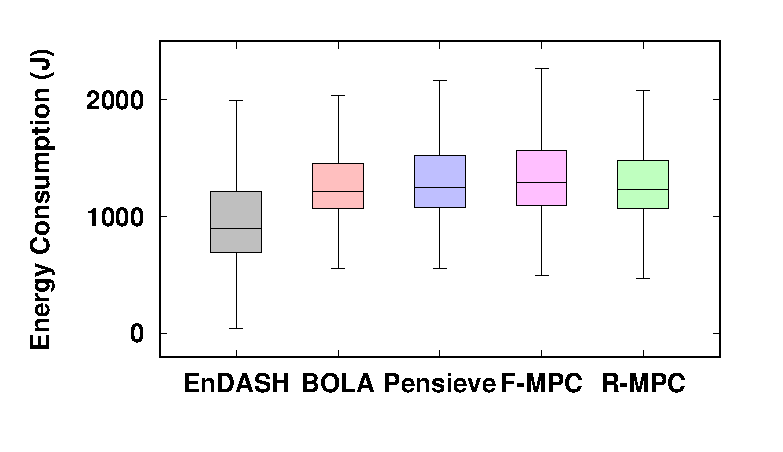
\includegraphics[width=0.33\textwidth]{new_results/simres/Energy}
		}
		\subfloat[\label{fig:chap04:EnDASH_QoE}QoE score (Eqn.~\ref{eq:chap04:QoE})]{
			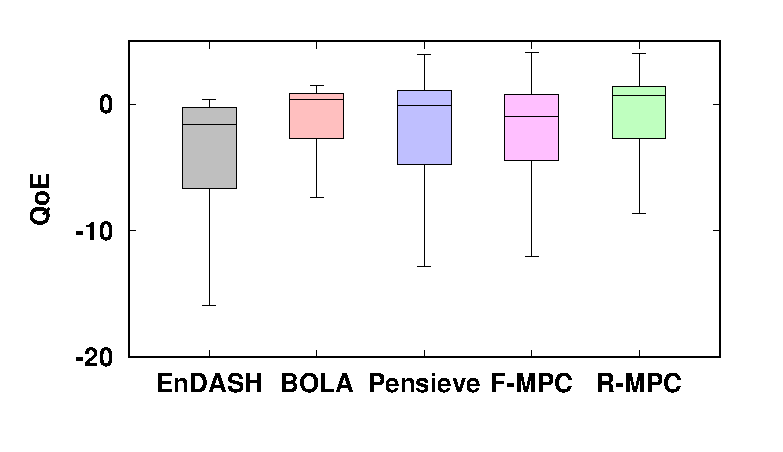
\includegraphics[width=0.33\textwidth]{new_results/simres/QoE}
		}
		\subfloat[\label{fig:chap04:EnDASH_buff}CDF of buffer length]{
			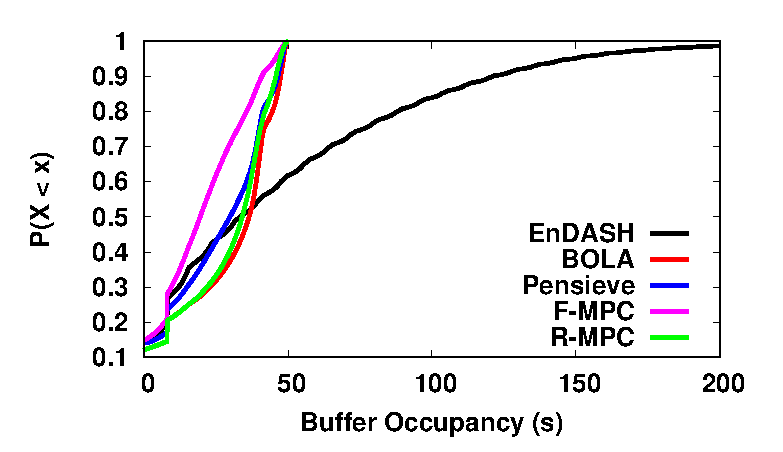
\includegraphics[width=0.33\textwidth]{new_results/simres/BuffOccu}
		}
	\end{center}
	\caption{\label{fig:chap04:EnDASH_vs_others}Performance comparison of EnDASH with baseline \ac{ABR} streaming algorithms, BOLA \cite{Spiteri2016}, Pensieve \cite{mao2017neural}, Fast MPC \cite{yin2015control}, Robust MPC \cite{yin2015control}}
\end{figure}
\begin{figure}[h]
	\captionsetup[subfigure]{width=0.49\linewidth}
	\begin{center}
		\subfloat[\label{fig:chap04:avg_bitrate}Avg. Bitrates in Mbps]{
			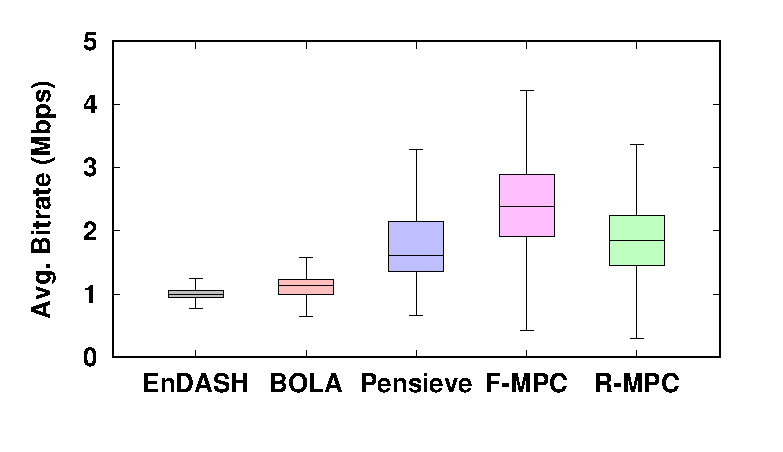
\includegraphics[width=0.49\linewidth]{new_results/simres/AvgBitrate}
		}
		\subfloat[\label{fig:chap04:stall}Stall Time per segment (in seconds))]{
			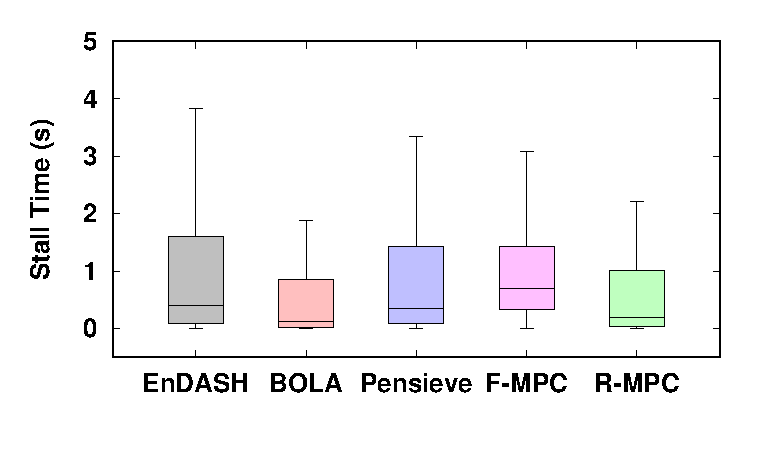
\includegraphics[width=0.49\linewidth]{new_results/simres/Stall}
		}\\
		\subfloat[\label{fig:chap04:smooth}Bitrate Variation]{
			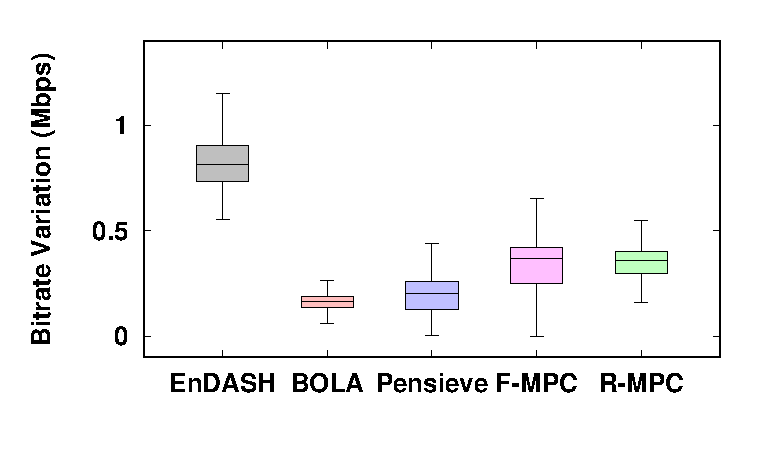
\includegraphics[width=0.49\linewidth]{new_results/simres/BitrateVar}
		}
	\end{center}
	\caption{\label{fig:chap04:indi_QoE}Comparison of different components of \ac{QoE} score (average bitrate, stall time, smoothness) of EnDASH with baseline \ac{ABR} streaming algorithms, BOLA \cite{Spiteri2016}, Pensieve \cite{mao2017neural}, Fast MPC \cite{yin2015control}, Robust MPC \cite{yin2015control}}
\end{figure}

\subsection{EnDASH versus Baseline ABR algorithms}
Fig.~\ref{fig:chap04:EnDASH_vs_others} shows the energy consumption, \ac{QoE} score, and buffer length variation of EnDASH and other baseline \ac{ABR} algorithms. For evaluating these algorithms, the length of each time slot is set to $T=30$ seconds, and the length of the historical window is also set to $x=30$ seconds, i.e., $\prefu{30}{30}$. %So, the average throughput for a prediction window of 30 seconds is predicted using the historical data of 30 seconds. 
In existing literature, the Pensieve \cite{mao2017neural} algorithm has been reported to generate optimal chunk bitrates and video quality. Fig.~\ref{fig:chap04:EnDASH_en} shows that EnDASH outperforms Pensieve in terms of energy consumption. However, this energy savings comes at the cost of sacrificing the \ac{QoE} with respect to Pensieve as seen in Fig.~\ref{fig:chap04:EnDASH_QoE}. Moreover, while the average QoE of EnDASH is comparable with the other algorithms, the inter-quartile range of \ac{QoE} is significantly high, implying that the corresponding variability is high.  
 \subsection{QoE Performance Analysis}
To understand the \ac{QoE} performance in detail, we plot the individual components of the \ac{QoE} metric in \fig{\ref{fig:chap04:indi_QoE}}. We observe that the mean of the average bitrate (Fig.~\ref{fig:chap04:avg_bitrate}) of EnDASH is smaller and its stall time (Fig.~\ref{fig:chap04:stall}) is comparable with other algorithms. However, the mean bitrate variation (Fig.~\ref{fig:chap04:smooth}) is much higher. Simultaneously, stall time displays a high variability. The reason for the reduced average bitrate, higher stall time variability, and higher mean of bitrate variation can be attributed to the tuning of the buffer length to the average throughput instead of the instantaneous throughput. For example, if the average throughput predicted is low, the system is forced to download a video chunk at a low bitrate for the entire timeslot, even though the throughput at multiple instances within the timeslot may be high, resulting in lower bitrates. Although the tuning to instantaneous throughput may improve bitrates, it will be associated with higher overhead. Hence, we focus on tuning to average throughput only. Further, the reduced inter-quartile range of the average bitrate is due to the aggressive fetching of video chunks. 
\subsection{Energy Performance Analysis}
EnDASH consumes much less energy because the video chunk download, and hence the playback buffer length, is tuned to the average predicted cellular network throughput. As a result, during high throughput conditions, the playback buffer length will increase, thereby facilitating the download of a higher number of chunks in a slot. This consecutive fetching of chunks reduces the tail energy which eventually manifests in the reduction of overall energy consumption as seen in Fig.~\ref{fig:chap04:EnDASH_en}. The resulting trade-off is reflected in the increase in buffer length in comparison with the buffer length of competing ABR algorithms.  Fig.~\ref{fig:chap04:EnDASH_buff} shows the CDF of playback buffer length of different algorithms. It is seen that while the maximum buffer length of existing algorithms is 50 seconds that of EnDASH can go up to 200 seconds; but this is a rare instance. In nearly 60\% of the time the buffer length remains below 50 seconds.

\begin{figure}[ht]%
	\centering
	{\fbox{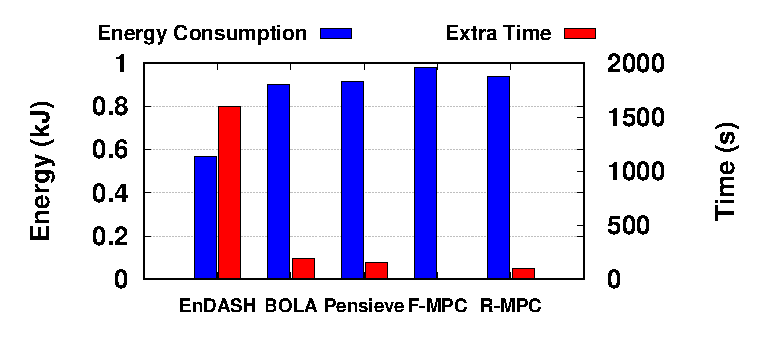
\includegraphics[width=0.7\linewidth]{new_results/simres/EnergyConsumption}}}	
	\caption{Energy Consumption and Extra Playtime obtained w.r.t. Fast MPC, which has the highest energy consumption}\vspace*{-0.5cm}
	\label{fig:chap04:vid_time_save}
\end{figure}
\subsection{Gain from Energy Savings}
\indent In this section, we discuss the gain in video playback time achieved by using EnDASH. FastMPC has the highest energy consumption among all algorithms. \fig{\ref{fig:chap04:vid_time_save}} shows the gain in video playback time achieved by the algorithms with respect to FastMPC while streaming a 2200 second video. It shows that using the energy saved by streaming the video using EnDASH, one can gain an additional 1403 seconds and 1440 seconds of video playback time in comparison with BOLA and Pensieve, respectively. Thus, one may infer that EnDASH can be used as a potential ABR streaming algorithm for increasing battery backup in smartphones.

\subsection{Feature importance study on throughput prediction engine} The primary objective of the throughput prediction engine is to account for the impact of cellular network technology change, i.e., the switching between 2G, 3G, 4G, etc., on network throughput.
\fig{\ref{fig:chap04:feature_imp}} shows the feature importance of different input parameters when predicting throughput. We observe that vertical handovers and associated technology (Network Type) have the highest weightage among all parameters, 0.32 and 0.21, respectively. The importance of such features in throughput prediction points out to
the absolute necessity of considering the existence of legacy systems when designing algorithms for 4G networks. 
\begin{figure}[!ht]
    \centering
    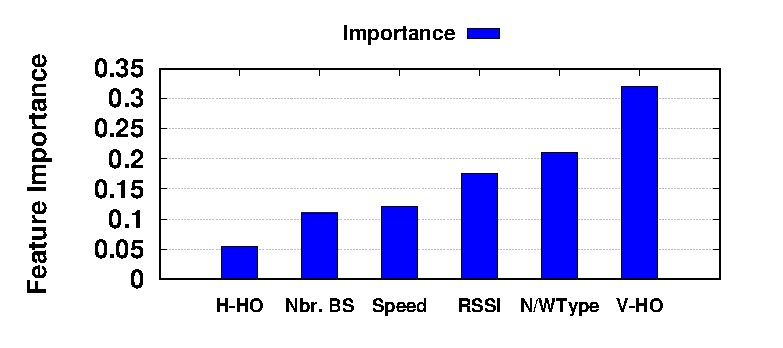
\includegraphics[width=0.7\linewidth]{new_results/simres/FeatureImpotance}
    \caption{Feature importance of the input parameters; signal strength, associated technology, and handovers (HOs)) between technology are the three features having the highest contribution in deciding throughput}\vspace*{-0.5cm}
    \label{fig:chap04:feature_imp}
\end{figure}
\begin{figure}[ht]
	\captionsetup[subfigure]{width=0.49\linewidth}
	\begin{center}
		\subfloat[\label{fig:chap04:MAPE_diff_scene}MAPE score measuring error of throughput prediction in different regions for various combinations of considering  associated technology and vertical handover (HO); for $\prefu{30}{30}$]{
			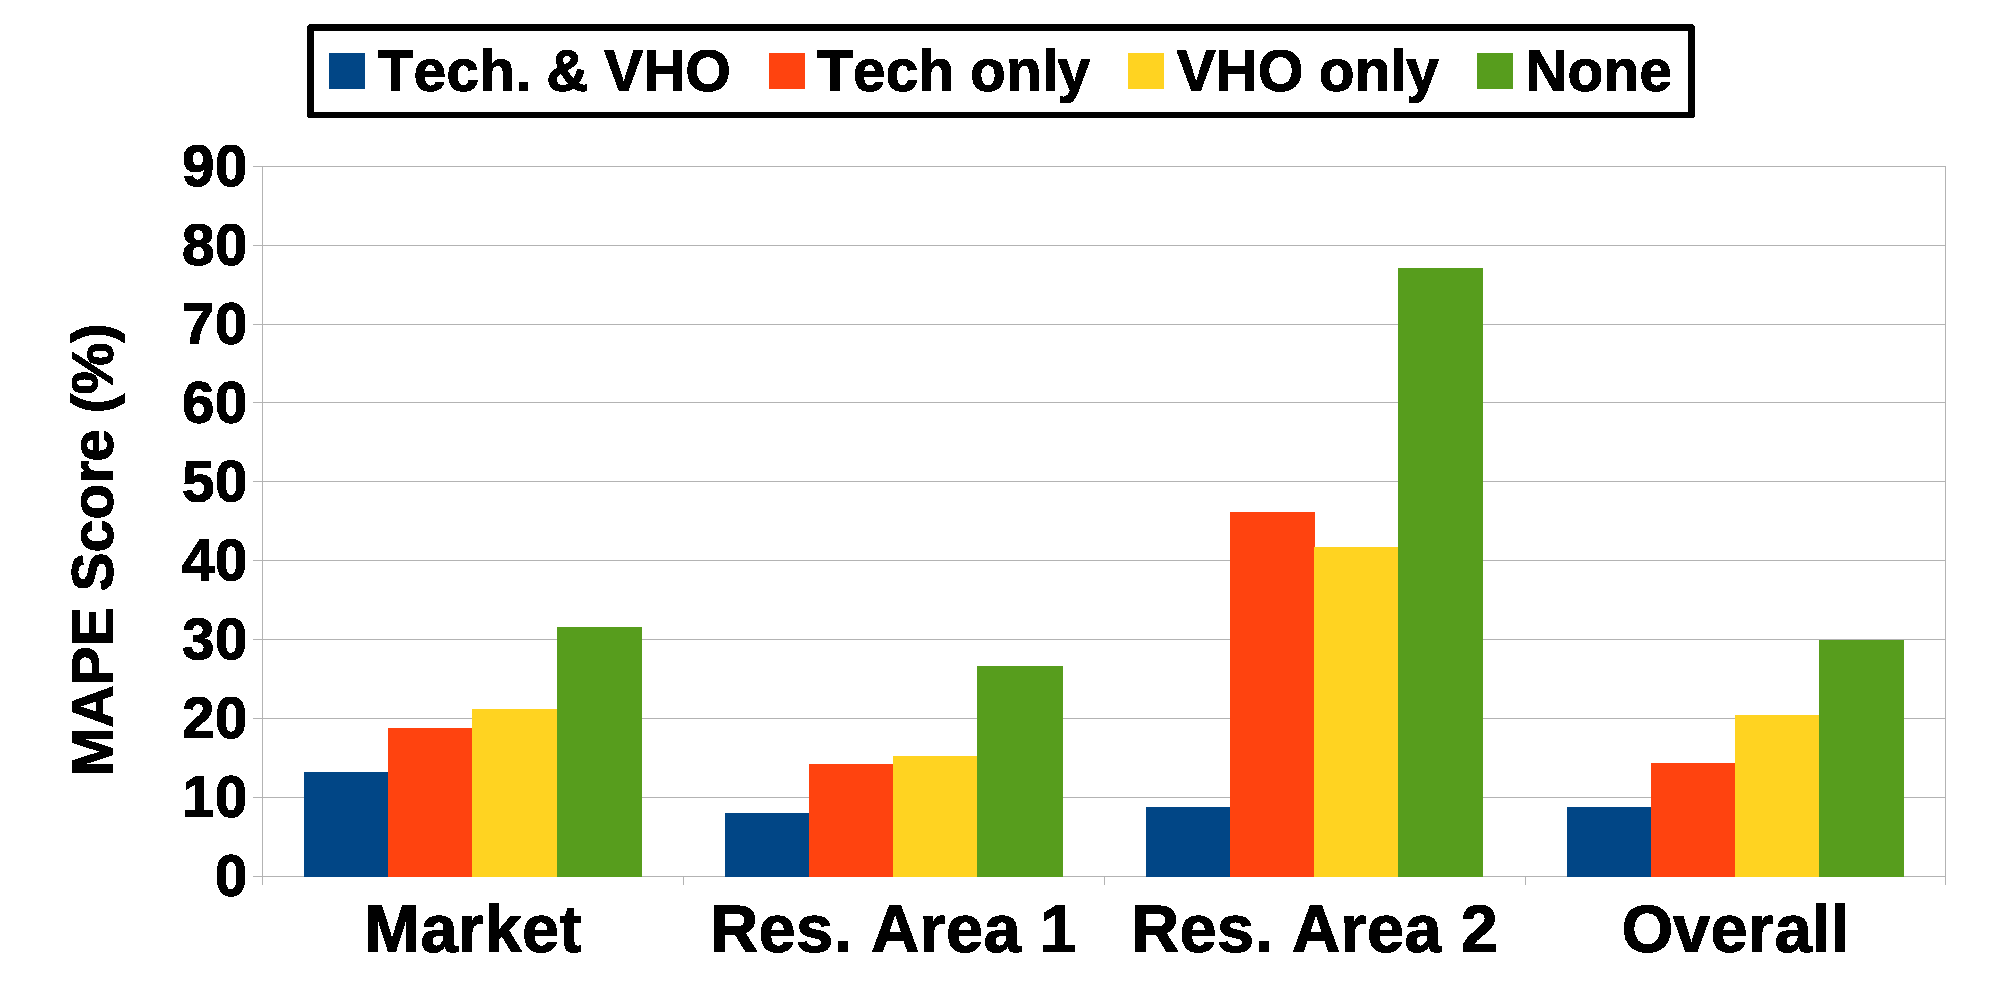
\includegraphics[width=0.49\linewidth]{figures/resi_vs_market_vs_overall_MAPE.eps}
		}
		\subfloat[\label{fig:chap04:Perf_VHO}Impact of considering associated technology and vertical handovers (HOs) on performance metrics of EnDASH; for $\prefu{30}{30}$]{
			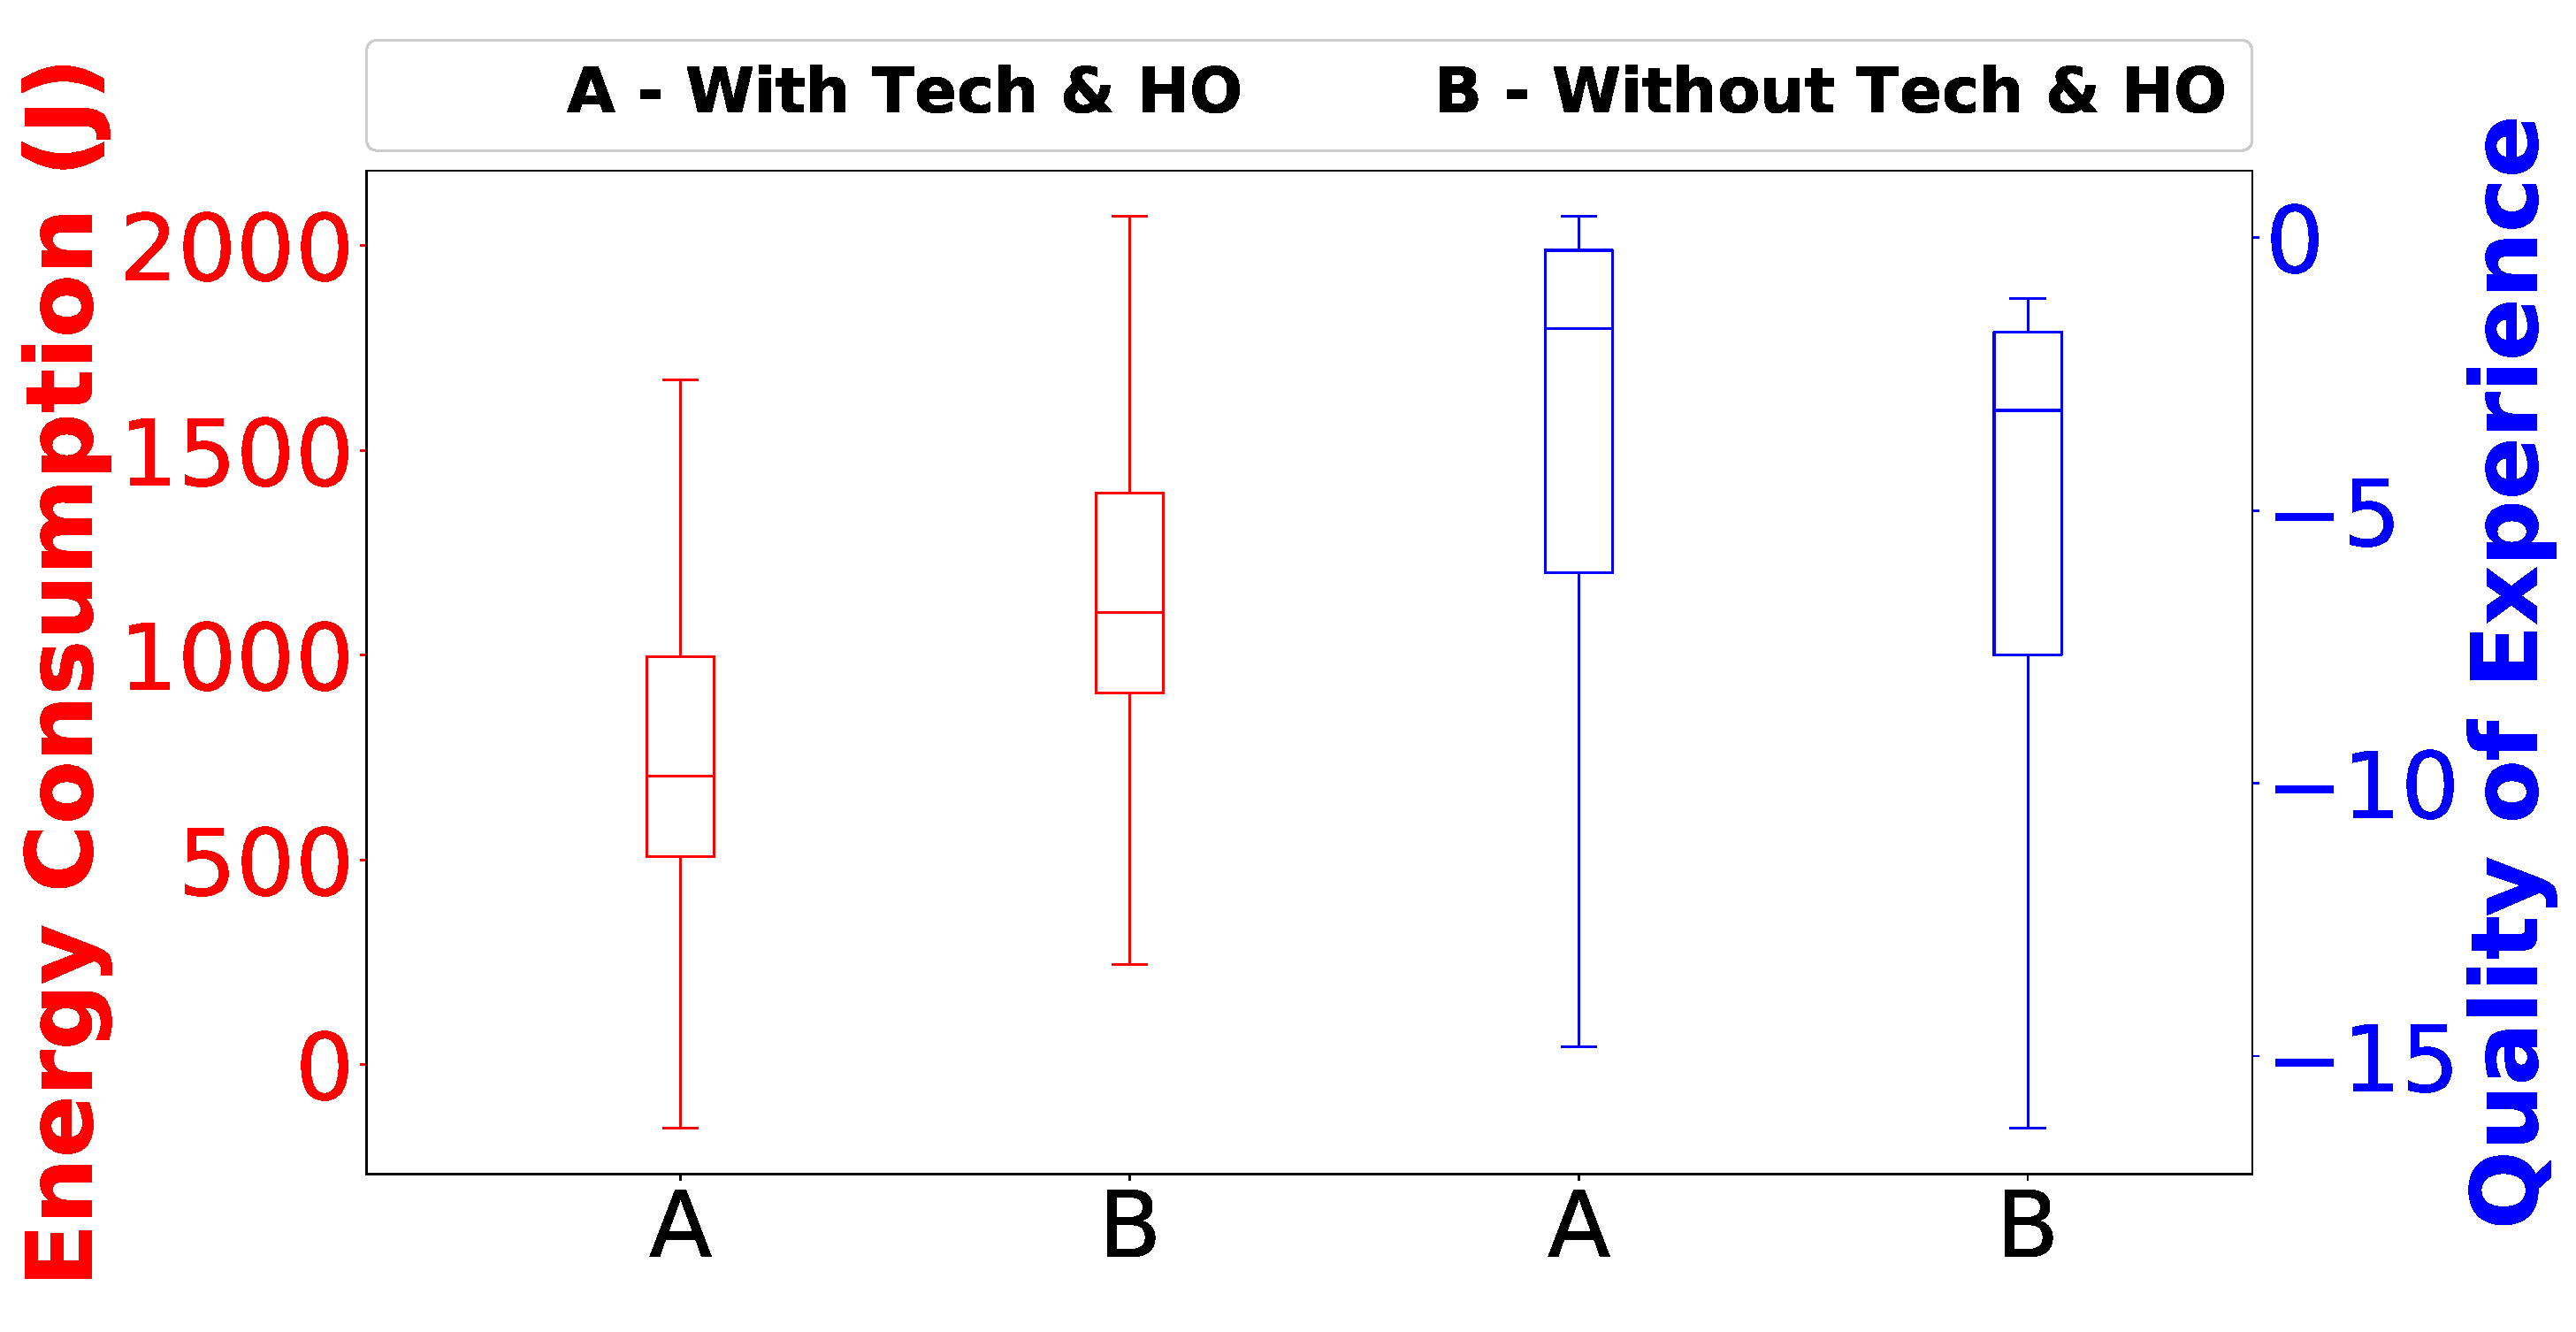
\includegraphics[width=0.49\linewidth]{figures/pow_qoe_comp.eps}
		}\\
		\subfloat[\label{fig:chap04:thpt_pred_trace}Predicted vs Actual throughput using the RF algorithm when associated technology and vertical handover (HO) is considered]{
			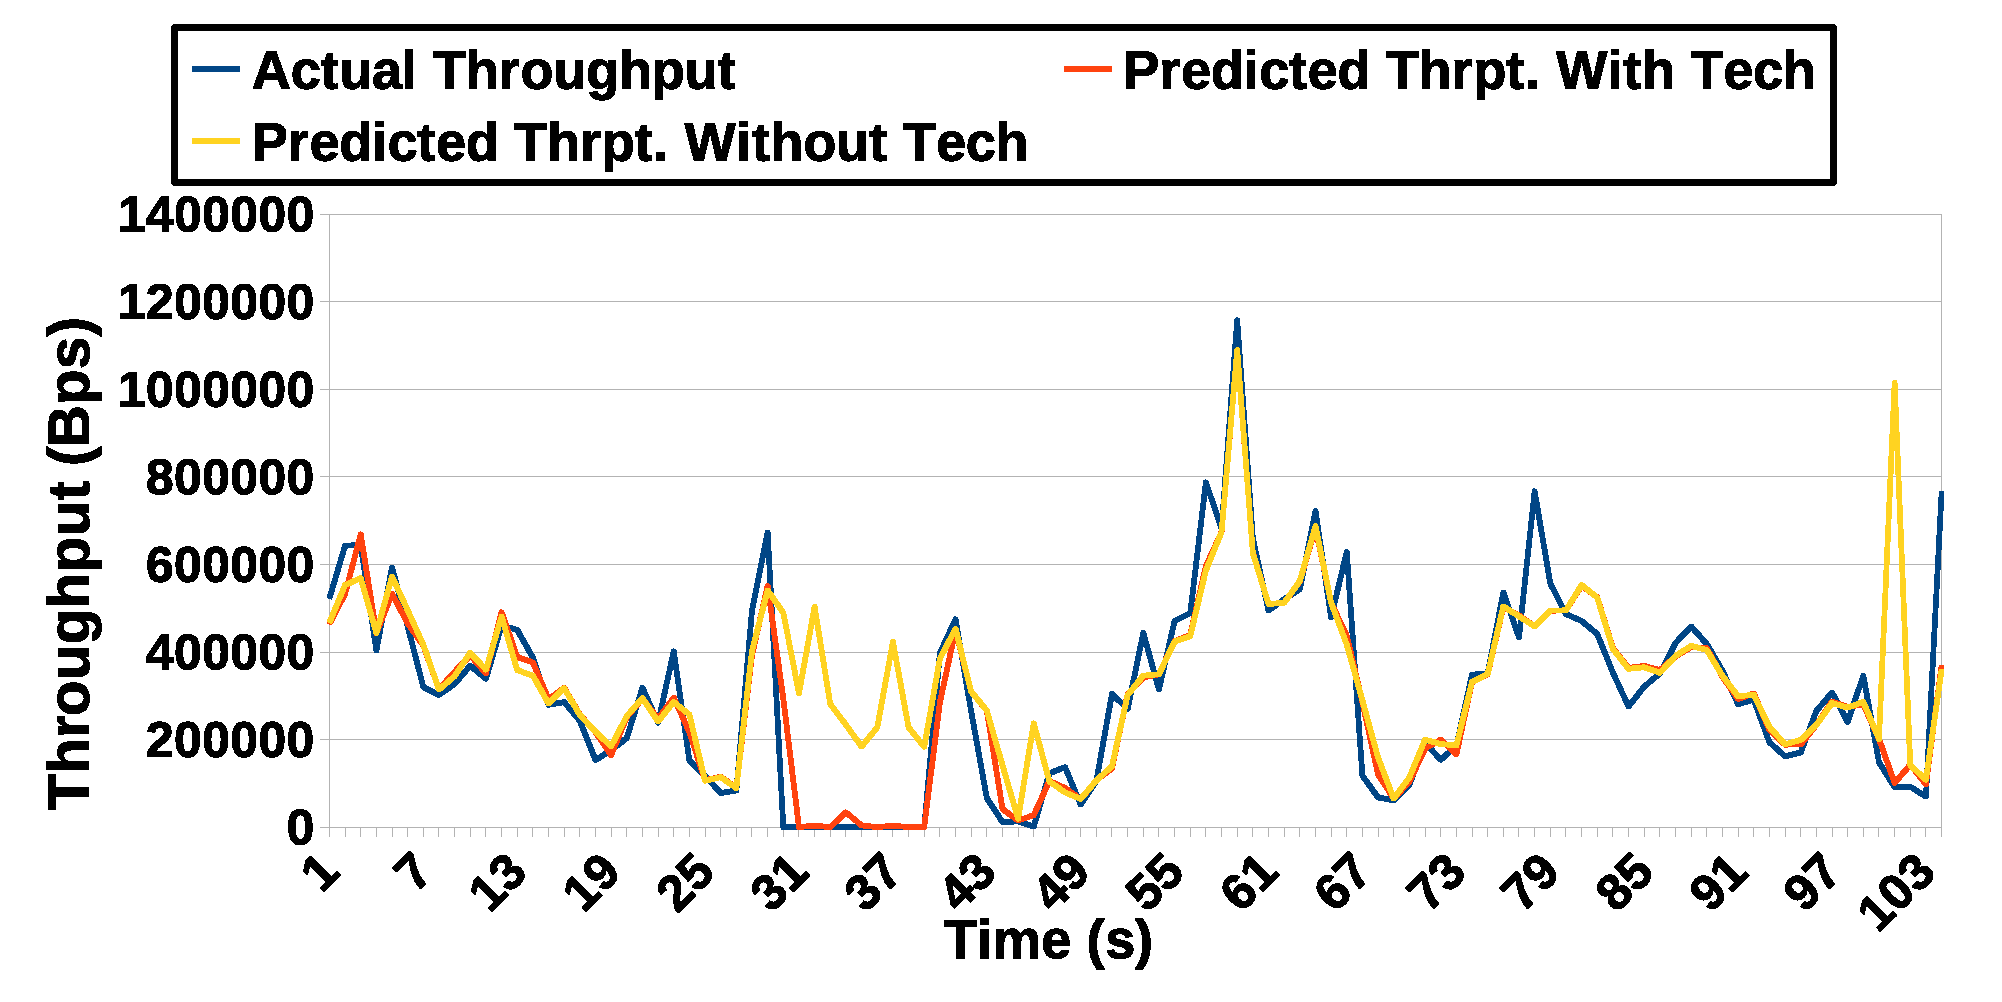
\includegraphics[width=0.49\linewidth]{figures/predicted_vs_actual_vs_Tech.eps}
		}
	\end{center}
	\caption{Effect of Associated Technology and Vertical Handovers (HOs) on Throughput Prediction and EnDASH performance for $\prefu{30}{30}$}
\end{figure}
%  \begin{figure*}[t]%
%\centering
%\subfigure[MAPE score measuring error of throughput prediction in different regions for various combinations of considering  associated technology and vertical handover (HO); for $\prefu{30}{30}$]{%
%\label{fig:MAPE_diff_scene}%
%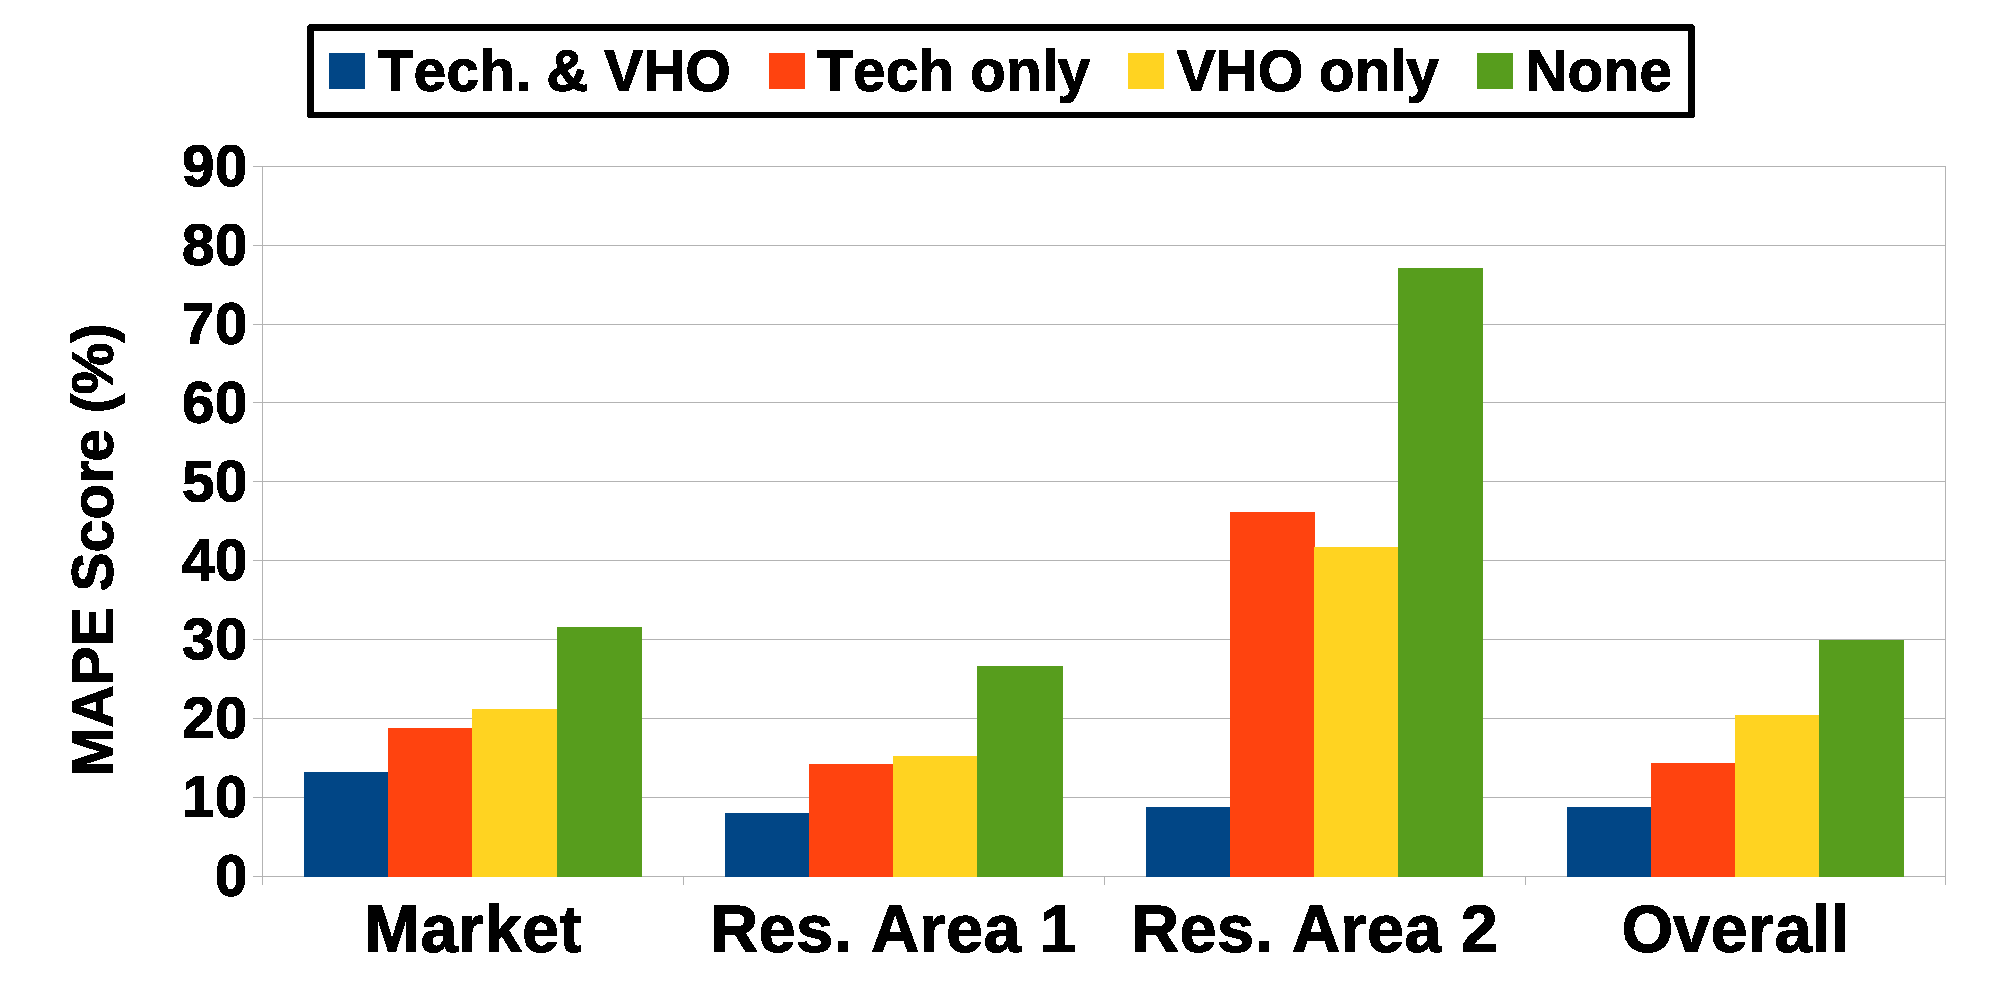
\includegraphics[width=0.3\textwidth]{figures/resi_vs_market_vs_overall_MAPE.eps}}
%\hspace{0.1cm}
%\subfigure[Impact of considering associated technology and vertical handovers (HOs) on performance metrics of EnDASH; for $\prefu{30}{30}$]{%
%\label{fig:Perf_VHO}%
%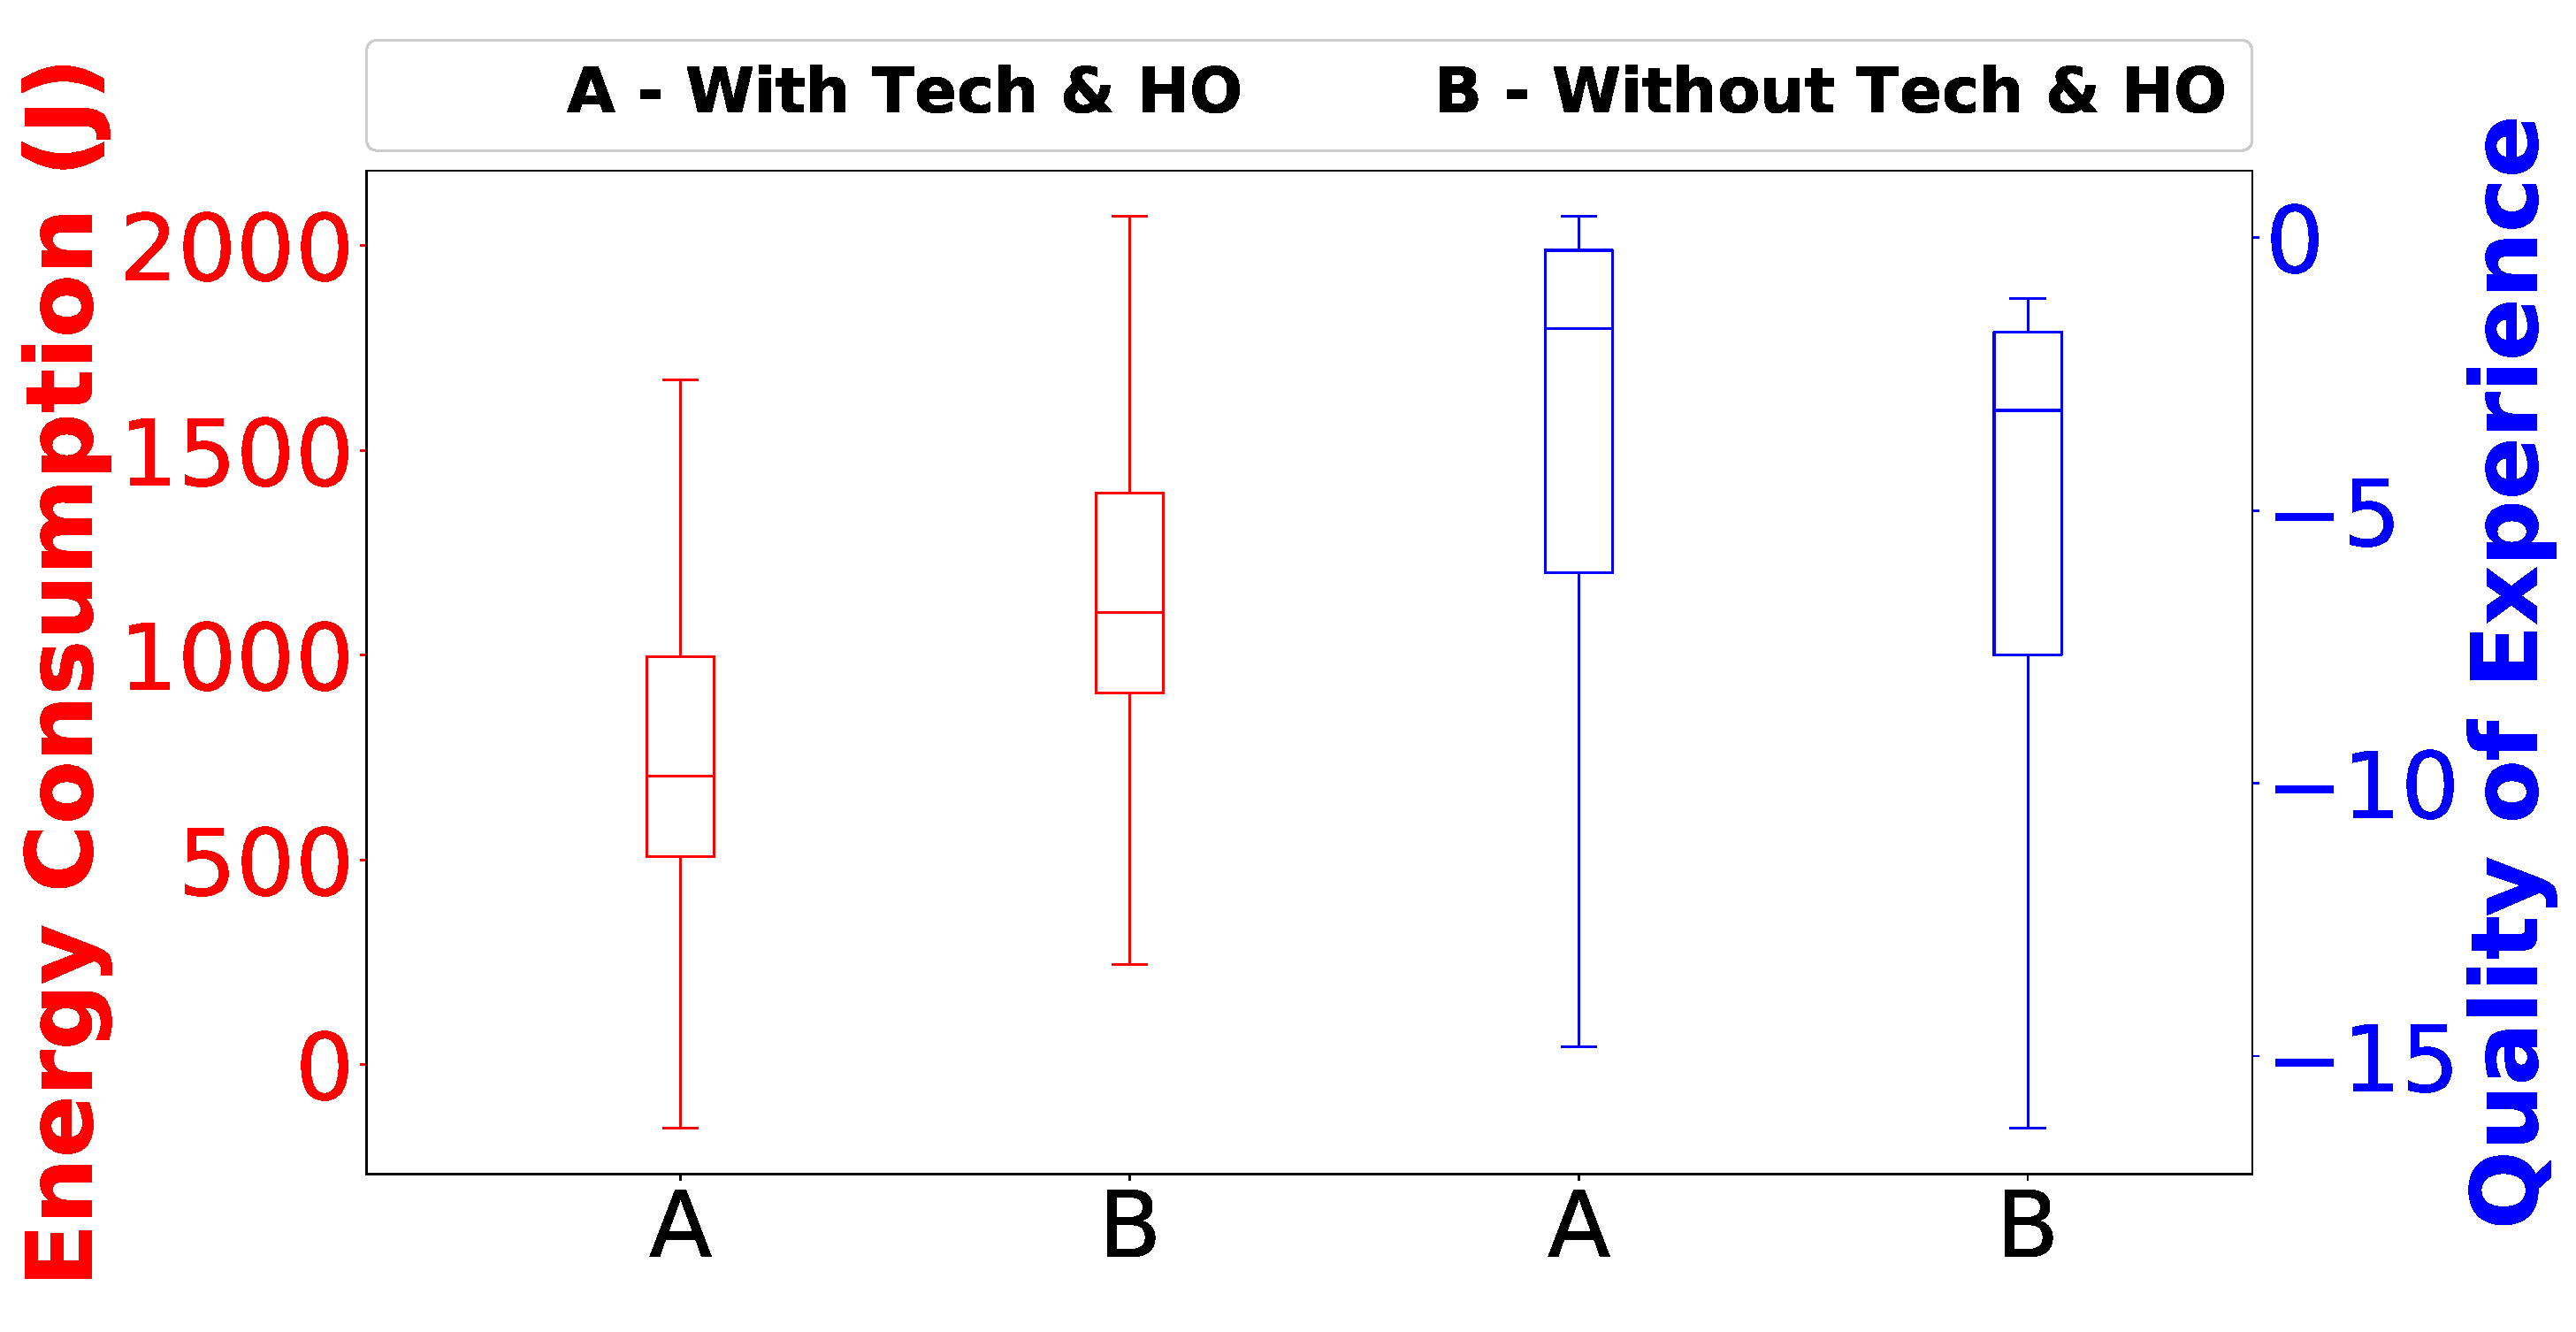
\includegraphics[width=0.3\textwidth]{figures/pow_qoe_comp.eps}}%
%\hspace{0.1cm}
%\subfigure[Predicted vs Actual throughput using the RF algorithm when associated technology and vertical handover (HO) is considered.]{%
%\label{fig:thpt_pred_trace}%
%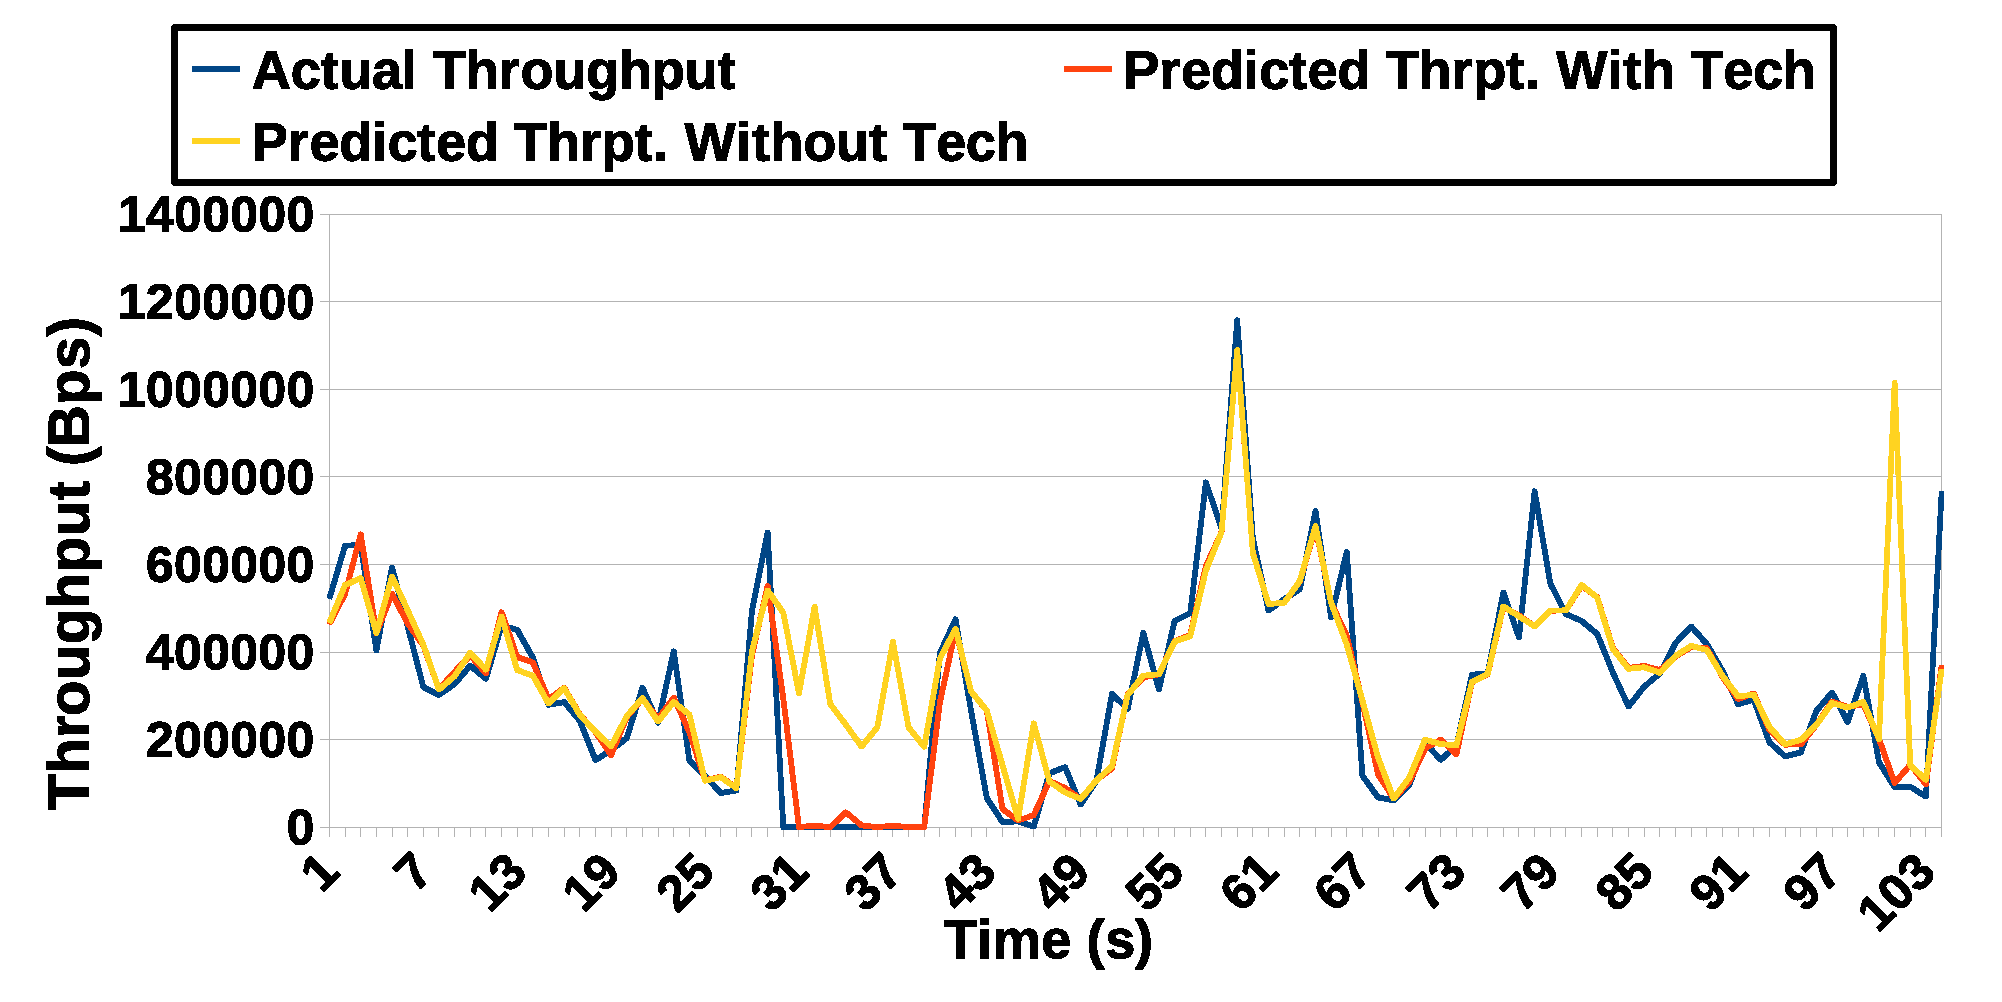
\includegraphics[width=0.3\textwidth]{figures/predicted_vs_actual_vs_Tech.eps}}%
%\caption{Effect of Associated Technology and Vertical Handovers (HOs) on Throughput Prediction and EnDASH performance for $\prefu{30}{30}$}\vspace*{-0.5cm}
%\end{figure*}
\subsection{Importance of Associated Technology}
\indent To understand the impact of associated technology and vertical handovers on the throughput prediction error, we have evaluated the MAPE~\footnote{\indent MAPE score, which quantifies error in throughput prediction,  is:
\begin{align}
\text{MAPE\ score} = \frac{1}{N}\sum_{i=1}^N\left|\frac{\tau_i-\hat{\tau}_i}{\tau_i}\right|\times 100\%
\end{align}
where $\tau_i$ and $\hat{\tau}_i$ respectively denote actual and  predicted throughput in the $\mathrm{i^{th}}$ timeslot.
} score over different regions. For this, we have divided the data traces collected in Kharagpur into three categories - (a) crowded Market Place, (b) a residential area with extensive 4G coverage (Residential Area 1), and (c) a residential area with limited 4G coverage (Residential Area 2). The overall MAPE score and the MAPE score for the three different scenarios, each with different combinations of associated network technology and vertical handover, is shown in \fig{\ref{fig:chap04:MAPE_diff_scene}}. It is observed that the lowest MAPE score is reported when the throughput prediction considers the associated technologies and vertical handovers, especially when 4G coverage is limited. 
\fig{\ref{fig:chap04:Perf_VHO}} shows how the inclusion of both associated technology and vertical handover as features in the throughput prediction improves the EnDASH performance, in terms of energy consumption as well as \ac{QoE}.\\
\indent The impact of associated technology can be further understood if we look into the actual throughput traces and its prediction, which \fig{\ref{fig:chap04:thpt_pred_trace}} shows.
We have generated  \fig{\ref{fig:chap04:thpt_pred_trace}} with $\prefu{30}{30}$.
It is observed that if the associated technology and the vertical handover is not considered then there is significant mismatch in low throughput regions where there is a tendency of over estimation of the throughput.

\section{\textbf{Conclusion}}\label{section:conclusion}
%In many developing countries, 4G coverage is not ubiquitous. As a result users often have to fallback to legacy networks that support lower throughput, resulting in a higher energy consumption and lower QoE. 
\acresetall
In this report, we propose EnDASH -- an energy aware ABR video streaming algorithm, which minimizes energy consumption while not compromising on QoE of users under mobility. It exploits the high throughput regions in the user's trajectory for aggressive fetching of video chunks thereby reducing energy consumption even in regions with limited 4G coverage and significant presence of legacy networks.  To achieve this, it intelligently tunes the playback buffer length with the average predicted throughput and then resorts to optimal bitrate selection for video chunks. As a result, the buffer length increases sometimes; although, the consequent cost  escalation is negligible. This is because the cost is incurred due to  (a) extra memory usage which is cheap  and can be ignored, and (b) aggressive fetching which may lead to some wastage, but such wastage is rare and minimal, therefore, hardly having any cost impact.\\  %Moreover, the data tariff is extremely cheap ; thus hardly having any impact on the cost.\\
\indent EnDASH predicts the cellular network throughput using Random Forest Learning. It tunes the buffer length and selects the optimal chunk bitrates using Reinforcement learning. EnDASH is able to improve the maximum energy consumption by about 30.4\% in comparison to the popular Pensieve algorithm although with reduction in QoE. Since EnDASH is a tunable algorithm it can be designed to adapt to a specific  requirement, such as energy or QoE -- this would be our immediate future work.  Additionally, our future work will also involve real-life implementation of EnDASH and investigating the corresponding improvement in energy efficiency.

\section*{Publications}

\subsection*{Submitted}
\begin{enumerate}[start=1,label={[\arabic*]}]
	\item \textbf{Abhijit Mondal}, Sandip Chakraborty, ``\textit{An End-to-end protocol over Heterogeneous Internet}'', submitted to Elsevier Computer Networks.
\end{enumerate}

\subsection*{Published:}
\begin{enumerate}[start=1,label={[\arabic*]}]
	\item Nishant Somy, \textbf{Abhijit Mondal}, Bishakh Ghosh, Sandip Chakraborty, ``\textit{System Call Interception for Serverless Isolation}'', in Proceedings of the annual conference of the ACM Special Interest Group on Data Communication (SIGCOMM) 2020 Demos and Posters, New York, USA, August 11 - 14, 2020.
	\item \textbf{Abhijit Mondal}, Sandip Chakraborty, ``\textit{Federated Adaptive Bitrate Live Streaming over Locality Sensitive Playback Coalitions}”, in the Proceedings of the Workshop on Network Application Integration/CoDesign (NAI '20), Association for Computing Machinery, New York, USA, August 11 - 14, 2020. 
	\item \textbf{Abhijit Mondal}, Sandip Chakraborty, ``\textit{Does QUIC Suit Well with Modern Adaptive Bitrate Streaming Techniques?}”, in IEEE Networking Letters, vol. 2, no. 2, pp. 85-89, June 2020.
	\item \textbf{Abhijit Mondal}, Basabdatta Palit, Somesh Khandelia, Nibir Pal, Jay Jayatheerthan, Krishna Paul, Niloy Ganguly and Sandip Chakraborty, ``\textit{EnDASH - A Mobility Adapted Energy Efficient ABR Video Streaming for Cellular Networks}'', in the Proceedings of 2020 IFIP Networking Conference (IFIP Networking), Paris, France, June 22-25, 2020.
	\item Vinnakota Venu Balaji, Naganithin Manne, \textbf{Abhijit Mondal}, Debarati Sen and Sandip Chakraborty, ``\textit{An Experimental Study of C-RAN Fronthaul Workload Characteristics: Protocol Choice and Impact on Network Performance}", in Proceedings of the 89th Vehicular Technology Conference (VTC2019-Spring), Kuala Lumpur, Malaysia, April 28 - May 1, 2019.
	\item \textbf{Abhijit Mondal}, Sourav Bhattacharjee, Sandip Chakraborty, ``\textit{Viscous: An End to End Protocol for Ubiquitous Communication Over Internet of Everything}'' in Proceedings of 42nd Annual IEEE Conference on Local Computer Networks (IEEE LCN 2017), Singapore, October 9-12, 2017.
	\item \textbf{Abhijit Mondal}, Satadal Sengupta, B.R. Reddy, M.J.V. Koundinya, Chander G., Pradipta De, Niloy Ganguly, Sandip Chakraborty, ``\textit{Candid with YouTube: Adaptive Streaming Behavior and Implications on Data Consumption}'' in Proceedings of the 27th Workshop on Network and Operating Systems Support for Digital Audio and Video (ACM NOSSDAV’17), Taipei, Taiwan, June 20 - 23, 2017.
\end{enumerate}


	


\clearemptydoublepage

\chapter[SpDASH]{Divide and Stream - A Split DASH Architecture for Improved ABR Streaming}
\label{chapter05}
\noindent

\renewcommand{\relpath}[1]{Chapters/05.SpDASH/}
\graphicspath{{Chapters/05.SpDASH/}}

\newcommand{\red}[1]{\textcolor{red}{#1}}
\newcommand{\bel}{\textit{Belovezha}}
\newcommand{\servname}{\textit{BiFrost}}
\newcommand{\cliname}{\bel\ client}
\renewcommand{\basabdatta}[1]{\textcolor{red}{\textit{\textbf{#1}}}}
\renewcommand{\jay}[1]{\textcolor{red}{{\textbf{#1}}}}
\newcommand{\krishna}[1]{\textcolor{blue}{{\textbf{#1}}}}
\newcommand{\am}[1]{\textcolor{blue}{#1}}
\newcommand{\notesc}[1]{\textcolor{red}{\textit{\textbf{#1}}}}

\section{Introduction}\label{sec:chap05:intro}
Video traffic over the Internet has increased many-fold in recent years with the growing popularity of various over-the-top (OTT) media services like NetFlix, HotStar, Hulu, Amazon Prime, etc., over the world. The OTT service providers take help of the content delivery networks (CDN) to host the video contents and use HTTP Adaptive Streaming (HAS)~\cite{}, mostly powered by Apple HLS~\cite{} and MPEG-DASH~\cite{}, at the core of the streaming mechanism. HAS helps the end-users to meet the quality of experience (QoE) for the video streaming based on the variability at the network bandwidth available to the streaming players for downloading the video contents. More specifically, the HAS algorithms measure the available bandwidth at the clients and requests for the video segments in one of the predefined quality levels (bitrates) such that the QoE objectives for the end-user can be ensured. Typically, the QoE for the end-users of OTT services is characterized through following four metrics~\cite{} -- (i) video start-up delay, (ii) average playback bitrate, (iii) bitrate variation during the video playback, and (iv) amount of rebuffering or playback-stalls. Indicatively, the end-users demand for high bitrate video streaming with zero rebuffering to have the best video playing experience, while having some importance on the start-up dely and the bitrate variation. 

Mobile OTT applications have seen a tremendous demand in the recent years, however, supporting interrupt-free high-bitrate video streaming over wireless environments, both with WiFi and cellular technologies, is a daunting challenge for the OTT service providers because of the high variability of the air-interfaces' throughput, both with WiFi and cellular technologies. Traditional buffer-based HAS techniques~\cite{} fail in such scenarios, as they make an estimate of the network condition by observing the average playback buffer occupancy at the streaming client. However, the average buffer length at the playback client does not provide the short-term efficacy of the wireless channel. For example, an instantaneous drop in the throughput due to an external interference in the wireless channel cannot be captured by measuring the average buffer length. However, such instantaneous variations can trigger a rebuffering, thus affecting the QoE of the end-users.  

To mitigate these problems, various recent literature~\cite{} have proposed machine learning (ML)-based toolboxes to decide the video bitrates depending on a number of parameters that might influence the network conditions. However, these approaches have two major limitations. (1) The bitrate selection algorithms used in HAS typically run at the client side. Running ML-based algorithms over handheld devices always have their cost implications in terms of resource consumption and energy-efficiency~\cite{}. Apart from the runtime costs, the pretrained model needs to be pushed at the client devices periodically, which also incur additional overhead. It can be noted that a server-support to run the ML model is not practically feasible, as the bitrate decision is taken for every video segments to be downloaded. Considering the typical segment length of HAS videos are in the range of a few seconds, the client needs very frequent server access, which can affect its performance. (2) Typically, the ML algorithms are sophisticated enough to get pretrained over a number of variable input parameters. However, if they are executed only based on the clients' local states, they may not be able to capture the accurate condition of the network~\cite{}. For example, existing studies~\cite{} show that a contention among multiple video streams from different clients, connected with the same WiFi access point (AP), results in unfair air-time distribution across the clients, resulting in poor QoE. The information about the number of clients currently sharing the total air-time is only available at the AP side, and not at the client side. Thus, only the client-side parameters may not make the model sophisticated anough to capture wireless channel variability. 

In this paper, we first perform a thorough study to show that the existing ML-based HAS mechanisms, like MPC~\cite{} and Pensieve~\cite{}, fail to correctly capture the wireless channel throughput when only the client states are used in the prediction model. Accordingly, in this paper, we propose an edge-assisted HAS mechanism for dynamic bitrate adaptation, called {\bel}, primarily targeting the wireless interfaces. In our approach, we take help of the last-mile access device, such as the WiFi AP, to decide the optimal bitrate for video streaming with an objective of maximizing the end-users' QoE. In {\bel}, we use a middlebox server, called {\servname}, that works as a proxy to run the bitrate selection algorithm on behalf of the clients associated with it, and then forwards the video download requests to the CDN server. However, such an architecture poses additional design challenges. Mobile clients trigger handovers from one \textit{point of association} (PoA), like the WiFi AP or cellular base stations, to the next. Therefore, the HAS client states preserved at {\servname} also need to be transferred from the current PoA to the next PoA. As this again posses additional overhead, ideally, we need a stateless mechanism for bitrate selection. In {\bel}, we develop a semi-stateful model for bitrate selection, such that the client handover incurs minimal cost in terms of state exchange between different {\servname} components. 

To further address the efficacy of {\bel} over existing HAS models, we developed a proof of concept (PoC) bitrate selection mechanism for the clients attached with a WIFi AP. We developed a ML model for bitrate selection based on the wireless channel states and connection-level parameters measured at the WiFi AP. It can be noted that one of the major advantages of {\bel} architecture is that it is client-agnostic. The client software does not need any modification depending on whether the device gets connected over a WiFi network or a cellular network. We only need the corresponding pretrained model to be pushed at {\servname} associated with the WiFi AP or the cellular base station.   

\notesc{Implementation and results ...}

In summary, our contributions in this paper are as follows. 
\begin{enumerate}
    \item From thorough analysis of WiFi channel states and its impact over the WiFi clients during video streaming, we show that the existing HAS bitrate selection models does not perform efficiently when only the client states are used for the optimal bitrate prediction. 
    \item We design and develop {\bel}, a middlebox at the edge, for optimal bitrate selection based on joint coordination between the client and its wireless PoA. 
    \item To reduce the overhead of {\bel}, we propose a semi-stateful model. \notesc{need to give further details about the novelty}. 
    \item We develop a PoC for ML-based bitrate selection using {\bel} over WiFi networks. \notesc{further details in terms of novelty} 
    \item \notesc{Contributions regarding implementation}
\end{enumerate}

\notesc{===TODOs=======}

\notesc{1. Over a WiFi setup, show that PenSieve and MPC fails to capture the correct bitrate based on only the states of the client. This can be a case study. Like play BBB from 10 clients associated with a AP, and show how WiFi channel variations impact bitrate selection. You may also show that the imput parameters of PenSieve does not correctly capture the wireless channel states.}

\notesc{2. Be careful about writing the methodology, use different figures, different terminologies, etc. from the patent document shared with Intel. Do not try to modify the architecture proposed in the patent -- write here from scratch.}

\notesc{3. Implement and test with WiFi networks. We need to develop a training model using the WiFi AP states, think about which parameters you'll take from AP. We need to show that this model works better than PenSieve and others.}

\notesc{4. Detailed analysis and results from implementation -- (a) emulation/simulation, (b) small-scale testbed. Brainstorm what graphs we want to give. Accordingly you can run the experiments to generate graphs.}

\vspace{1cm}
\notesc{\Large{\textbf{== Old Intro ===}}}


To improve the performance of \ac{DASH}, which is the primary video rendering protocol in recent times,  several \ac{ABR} video streaming algorithms have been proposed. Some of these algorithms, such as Pensieve \cite{Mao2017}, use \ac{ML} to decide the most optimal bitrates for video download. However, a deep rooted concern associated with the unbridled use of \ac{ML} algorithms in such applications as video streaming is the feasibility in their deployment. Particularly, in many emerging countries like India, a major section of the society uses medium budget smartphones with limited specifications. These phones may not, therefore, be capable of handling the requirements associated with running an \ac{ML}-equipped \ac{ABR} streaming algorithm.\\
\indent For example, for each video played by the client, Pensieve \cite{Mao2017} needs a trained model to decide the optimal download bitrate for the next video segment. This implies that  a different trained model should be stored for each video, which escalates the storage requirement. The alternative is online retraining of the algorithms, which again needs a huge amount of computational resources for delivering timely and accurate results. As DASH uses a dumb server and a smart client, both of the aforementioned solutions are to be implemented in the smartphones, i.e., where the client video player resides.  If the phones, however, have low memory and insufficient computational resources then \ac{ML}-assisted \ac{ABR} algorithms can trigger scalability issues.\\
\indent Algorithms like Pensieve \cite{Mao2017}, Oboe \cite{Akhtar2018}, HotDASH \cite{Sengupta2018} require an  ABR server which hosts and runs these algorithms. To minimize the time taken in information exchanges between the \ac{ABR} server and the client, \cite{Mao2017,Akhtar2018,Sengupta2018} propose that the \ac{ABR} server be located at the client itself. This implies that a local server be run at the end-devices, i.e., the smartphones, one for each player, which further leads to scalability concerns.\\
% chooses the download bitrate of the current video chunk as a function of the last chunk bitrate and some other parameters. However, in cellular networks, the chunk bitrate depends on the channel throughput. In such cases, the channel coherence time i.e., the time over which the channel response remains unchanged may be significantly smaller than the inter video segment download time.  For example, in 5G the channel coherence time is in the order of miliseconds ~\cite{}, whereas the time between two successive video segment download is in the order of seconds. Consequently, choosing the current chunk bitrate as a function of that of the last chunk may lead to erroneous decisions.
% \indent To ensure convenient deployment of \ac{ML} algorithms for optimal video streaming, in this paper, we have proposed a modification to the \ac{DASH} architecture while not altering the fundamental philosophy of \ac{DASH}. \\
\indent \ac{DASH} provides a low-complexity common ecosystem of networks and services obliterating the proprietary content silos. However, it solicits some modification for exploiting the benefits offered by \ac{ML}-assisted \ac{ABR} streaming algorithms, particularly for supporting such algorithms in medium and low budget phones. However, the ubiquitous usage of \ac{DASH} implies that any  modification must not alter the fundamental philosophy of \ac{DASH}, wherein the control lies with the client which takes the decisions for selecting the optimal next chunk download bitrates for individual users. \\
% \indent In the conventional \ac{DASH} architecture a target video is first encoded and then fragmented into chunks of fixed playback time. These chunks are stored at a \ac{CDN} server. The encoding ensures that the video player can distinguish between each chunk separately. There is a video player at the client side. The client takes stock of the current network bandwidth and the playback buffer of the video player. The \ac{ABR} streaming algorithm at the client side uses a combination of one or more of these metrics to decide the download bitrate of the next video chunk. So, in conventional DASH  the server is relieved of any additional workload associated with the choosing the optimal next chunk download bitrate for individual users. The entire control lies with the client side. \\
    \indent Our proposed modification, named \bel\ \footnote{Belovezha Accords is an agreement declaring the cessation of existence of USSR and hence the splitting of the same.}, splits the \ac{DASH} decision making engine. It replaces the smart client with a dumb client and introduces a middlebox in the form of an intelligent proxy server between the \ac{CDN} server and the client. We call the intelligent server \servname\footnote{\servname\ is the bridge connecting Asgard, the world of Gods, to Midgard, the world of humanity.}. \servname\ may be co-located either with a \ac{CDN} server  or the cellular network base-station. In either case the introduction of \servname\ does not disturb the organization of the host. \servname\ houses the \ac{ABR} server of~\cite{Mao2017,Akhtar2018,Sengupta2018} and is equipped with advanced technical parts for training the \ac{ABR} algorithms inside the \ac{ABR} server.  Thus, \bel\ offers the advantage of incorporating \ac{ML}-based \ac{ABR} streaming algorithms with DASH, without overwhelming the client. In fact, splitting the \ac{ABR} decision making engine from the client implies that the client requires no (a) add-on installation (\ac{ML} algorithms often have library dependencies that may not be well-defined for smartphones) , or (b) high-end features. Although targeted towards smooth incorporation of machine learning in \ac{DASH} \bel\ is expected to perform equally well non-\ac{ML} equipped \ac{ABR} algorithms.\\
    \indent In this work, we have implemented  the \bel\ client as an android application using HTML5 and Javascript. The \bel\ moderator-server - \servname\ has been developed in Python as an HTTP server with several special features. This bypasses the need to restructure the existing \ac{ML}-based ABR algorithms for training in smartphones, thereby extending the service to phones with limited features. Moreover, since a much higher number of cores can be made available in the server than the smartphone, hence, accurate bitrate decisions can be delivered in much less time. Our experimental results reflect that \bel\ performs at par with the unified \ac{DASH} architecture for ML-based ABR algorithms as well as other algorithms.  \\
    \indent It is, thus, evident that \servname\ is a middlebox. Although middleboxes introduce new functionalities, they often become bottlenecks due to proprietary control or increase in information exchange. So, several existing works \cite{Sherry2012} argue in the favour of doing away with middleboxes altogether. However, we have designed \servname\ simply as a plugin module. It does not have any proprietary control. Besides, our experiments show that there is no significant increase in the control channel overhead associated with \servname. It can, therefore, be used as a simple solution for improving user experience.

% In recent times, there has been an increase in the popularity of machine learning algorithms for the selection of optimal bit rates in \ac{DASH} 
% %stimulated by availability of low cost smartphones, affordable data plans, and a variety of  content on OTT video platforms,
% online video streaming has emerged as one of the most popular modes of entertainment. Most video users stream online videos in their smartphones over the mobile Internet. Hence, a stable mobile connection quality is integral to a satisfactory video viewing experience. However, the mobile connection quality is susceptible to random fluctuations, especially for travellers. A user under mobility in one instance may experience a 4G connection quality, in the next instance it may have to fallback to legacy 3G or 2G networks, or may have to pass through a connection blind spot with no reception at all. Such fluctuations introduce interruptions in the video playback, which reflect into a poor \ac{QoE} for the user. Provisioning a high \ac{QoE} to video users in the face of the fluctuating network conditions is one of the principal challenges encountered by network engineers and service providers.\\
% \indent Currently, video service providers serve video content using the \ac{DASH} protocol. In \ac{DASH}, a target video is stored at a \ac{CDN} server  after first being encoded in different qualities and then broken into chunks of equal playback times. The encoding ensures that the video player can understand each video chunk independently. A DASH video player, usually the client at the user end, estimates the current network bandwidth as well as the playback conditions and then employs an \ac{ABR} video streaming algorithm to determine the quality of the next video chunk to be fetched.\\
% \indent An incorrect estimate of the bit-rate may significantly deteriorate the \ac{QoE} of the user. For example, a high bit-rate estimate in the face of poor network conditions can increase the rebuffering time. Additionally, incessant bitrate variations (or less smoothness) between adjacent chunks or streaming at a lower bitrate also affects the \ac{QoE}. To this end, \ac{ABR} streaming algorithms optimizes the bitrate selection over three conflicting objectives - (a) high bitrate, (b) less rebuffering time, and (c) high smoothness. Popular \ac{ABR} algorithms such as MPC \cite{Yin2015}, BOLA \cite{Spiteri2016}, Pensieve \cite{mao2017neural}

% \noteng{The exact problem statement is introduced a bit late, Consider coming to the point may be after the first three paragraph. In general written well. }
\section{Related Work}\label{sec:chap05:related_work}
Existing ABR algorithms use different input parameters with different weightage to decide the optimal bitrates for improving user QoE. Some popular categories of \ac{ABR} algorithms are: 
\begin{enumerate}
    \item Buffer-based - which take the decision based on the playback buffer status~\cite{Spiteri2016,Huang2014}.
    \item Rate based - which estimate the network throughput from  previous chunk downloads to decide the throughput of the current chunk~\cite{Jiang2014,Xu2015}.
    \item Hybrid - which use both the buffer status and rate information to take bitrate decisions \cite{Zou2015}.
    \item QoE metric based - which are designed as  optimization problems for maximizing the user's QoE metric~\cite{Yin2015,Qin2018,Qin2019,Mao2017,Akhtar2018}.
\end{enumerate} 
\cite{Mao2017,Akhtar2018,Sengupta2018,Bampis2018,8816854,Huang2019} are neural network based \ac{ABR} streaming algorithms.  \cite{Mao2017} is one of the earliest papers to use A3C based recurrent neural network for deciding chunk bitrates that optimize QoE. \cite{Akhtar2018} improves \cite{Mao2017} by auto-tuning of parameters. \cite{Sengupta2018} uses reinforcement learning to identify user preferred hotspots in a video and render them at higher bitrates. \cite{Huang2018} uses deep reinforcement learning to achieve a high video quality with reduced transmission bitrates as well as at lower latency. \cite{Huang2019} uses a GAN (Generative Adverserial Network) based deep reinforcement learning algorithm in which agents compete with each other based on a set of rules to arrive at optimal bitrate decisions. \cite{Huo2019} optimizes the QoE of multiple users by learning the diversity in user's QoE requirements using a meta learning approach. \cite{Alt2019} proposes a sparse Bayesian Contextual Bandit Algorithm for designing optimized ABR streaming algorithms in Named Data Networks (NDN). \cite{Bampis2018} uses recurrent neural networks for subjective QoE prediction as a time-series problem.\\
\indent However, these works do not investigate the implementation aspect of the ML-assisted ABR algorithms. In several recent works, edge computing has been used to offload computationally intensive tasks  of IoT or mobile devices. \cite{Guo2019} uses joint computation and communication for proposing an optimal ABR algorithm using mobile edge networking over a fluctuating wireless channel. However, an inherent assumption in the work is the availability of the video at the edge server.\\
\indent In contrast, the \bel\ architecture proposed in our work has been designed to be compatible for any network, such as cellular communication networks or edge networks. In the current cellular network scenario it can be placed at the base-stations or the \ac{CDN} servers. For the future edge networks it can be placed in the edge nodes. Since it is a plug and play module, it can be used over a wide range of networks.

% Buffer-based ABR Streaming: [9] proposes a buffer-occupancy based ABR streaming algorithm which always maintains the playback buffer above 5 seconds duration. Additionally, it chooses the highest bitrate when the buffer has a 15 second cushion. Authors in [13] provide theoretical justification that buffer based algorithms yield better performance than those which need bandwidth occupancy information. In addition they also propose BOLA, a utility maximizing buffer occupancy based ABR video streaming algorithms. The utility function is defined considering all the QoE components.
% Rate-based ABR Streaming:   These algorithms estimate the network bandwidth during the last chunk download and use it as the throughput of the current chunk. The bitrate for the current is chosen from this estimated throughput. An example of a rate-based ABR streaming algorithm is Festive which predicts the throughput of the current chunk as the harmonic mean of the previous five chunks. The highest bitrate below this estimated throughput is chosen as the current bitrate [14]. Authors use a Kalman filter to predict the network throughput in [16].
% Joint Buffer and Rate based ABR video Streaming: [10, 12, 17] propose ABR streaming algorithms which consider both buffer occupancy and current chunk or network throughput to select optimal bitrates for future video chunks. Fast MPC in [10] optimizes the QoE for the next five video chunks based on the past network throughput and buffer occupancy. Robust MPC in [10] further improves fast MPC by exploiting the errors between the actual and the predicted throughputs of the past five chunks. 
% Neural Network based ABR video Streaming:  Of late, neural network based learning algorithms have gained popularity in terms of delivering a high QoE through the choice of optimal bit rates. Authors in [8] propose Pensieve, an ABR streaming algorithm which uses reinforcement learning (RL) algorithm to select optimal bitrates that maximize over a QoE metric.  In [14] authors propose a reinforcement learning based ABR streaming algorithm which renders video segments of higher user interests called hotspots at higher rate than others.
% In [12] authors propose Oboe, which is proposed to work atop algorithms like BOLA, Pensieve, MPC, etc. Oboe first prepares an offline model which sets the parameters of the aforementioned algorithms according to different network states. It then applies change point detection algorithm on network states to tune the parameters of these algorithms
% [8-16] propose ABR streaming algorithms which attempt to improve QoE exploiting various parameters such as playback buffer length, estimated network throughput, etc.


%\section{Pilot Study}
\section{The Proposed Belovezha Architecture}\label{sec:chap05:proposed_work}
\begin{figure}[h]
    \centering
    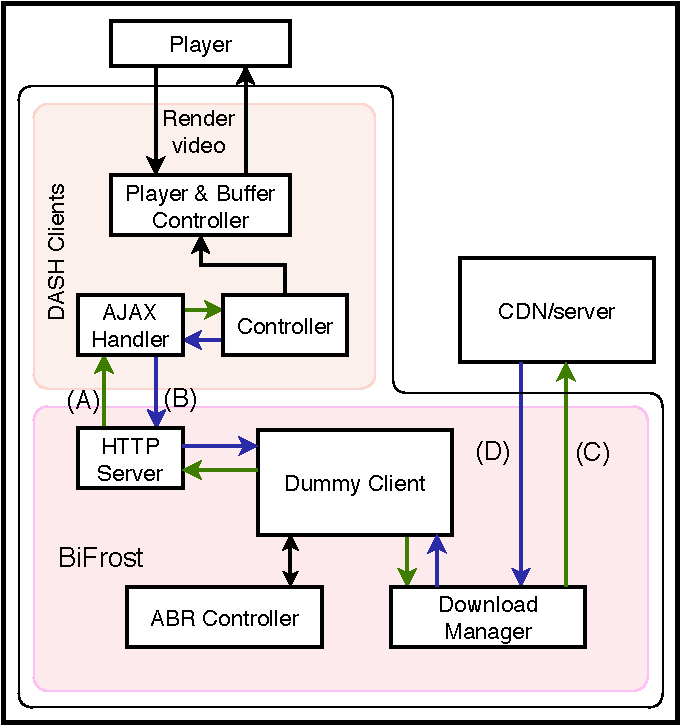
\includegraphics[width=\linewidth]{./images/playerDiagram_split.pdf}
    \caption{Proposed \bel\ architecture - a Split DASH model. There is a Dumb DASH Client at the user end and a Smart DASH Intelligent Proxy Server, \servname\, between the CDN server and the client.}
    \label{fig:chap05:splitDASH}
\end{figure}
In this section, we explain the architecture of \bel, which comes with the following major modifications in the DASH architecture:
\begin{enumerate}[(i)]
    \item the smart \ac{DASH} client is replaced with a dumb client in \bel , and
    \item an intelligent DASH proxy server, named \servname\, is introduced between the \ac{CDN} server and the client.
\end{enumerate}\
The resulting \bel\ architecture is shown in Fig.~\ref{fig:chap05:splitDASH}. The dumb client does not take any decisions related to the choice of the chunk bitrates. It simply controls the video playback while depending on \servname, to fetch the chunks from the CDN server. To assist \servname\ in taking bitrate decisions for future video chunks and delivering the same, the client reports - (a) its current playback buffer status, \am{(b) current playback time, (c) total stall time} and (d) its previous download history, to \servname\ every time it sends a request to \servname\ for video-segment download. \\
\indent \textcolor{red}{AM: Every time \servname\ receives a request from the client, it combines the information sent by the client into a `\textit{server state}'}. \textcolor{blue}{ It uses this server state to decide the audio and the video quality of the next video chunk to be downloaded. It has been discussed earlier that \servname\ will be co-located either with a  \ac{CDN} server or a \ac{BS}. However, during the course of travel, a mobile user does not connect to the same \ac{CDN} server or \ac{BS}. Evidently, it will not always connect to the same \servname\ server, for which the latter has been designed to be stateless.  So, \servname\ forwards the previous download history (received earlier from the client) to the client along with the current video segment. In addition, it also sends the time the client must wait before sending the next request for segment download.\\
\indent The next two sections provide a detailed description of the design and functioning of both the \bel\ client and the server.} 
\subsection{The Belovezha Client}
The \bel\ client has three fundamental modules - a) a playback and buffer controller, b) a client controller and c) an AJAX manager. 
\subsubsection{Playback and Buffer Controller}
    The \textit{playback and buffer controller} controls the video playback at the native player using the Source Buffer APIs of HTML5 Media Source Extension. It acts as an interface between the native player and the client controller.
\subsubsection{Client Controller}
The \textit{Client controller} supervises the functioning of the entire client. It starts the moment the client starts up and  initiates communication with the \bel\ server - \servname. It prepares all the requests to be sent to \servname, parses the received responses, and then  follows the instructions received. When the response contains any media segment, it feeds the media segment to the buffer controller. The client controller also maintains a record of the playback buffer status, and the current segment download information over link between the client and \servname.
\subsubsection{AJAX Controller}
The \textit{AJAX controller} handles the communication between \servname\ and the client. It monitors the communication continuously and records all the events. If a communication stays unresponsive for a threshold time, it aborts the communication and starts it again. The AJAX controller aborts communication by itself instead of relying on the native connection timeout mechanism to have more control, which makes the client robust and tolerant to network failures.
\subsection{The Belovezha server - BiFrost}
\begin{figure*}[h]
    \centering
    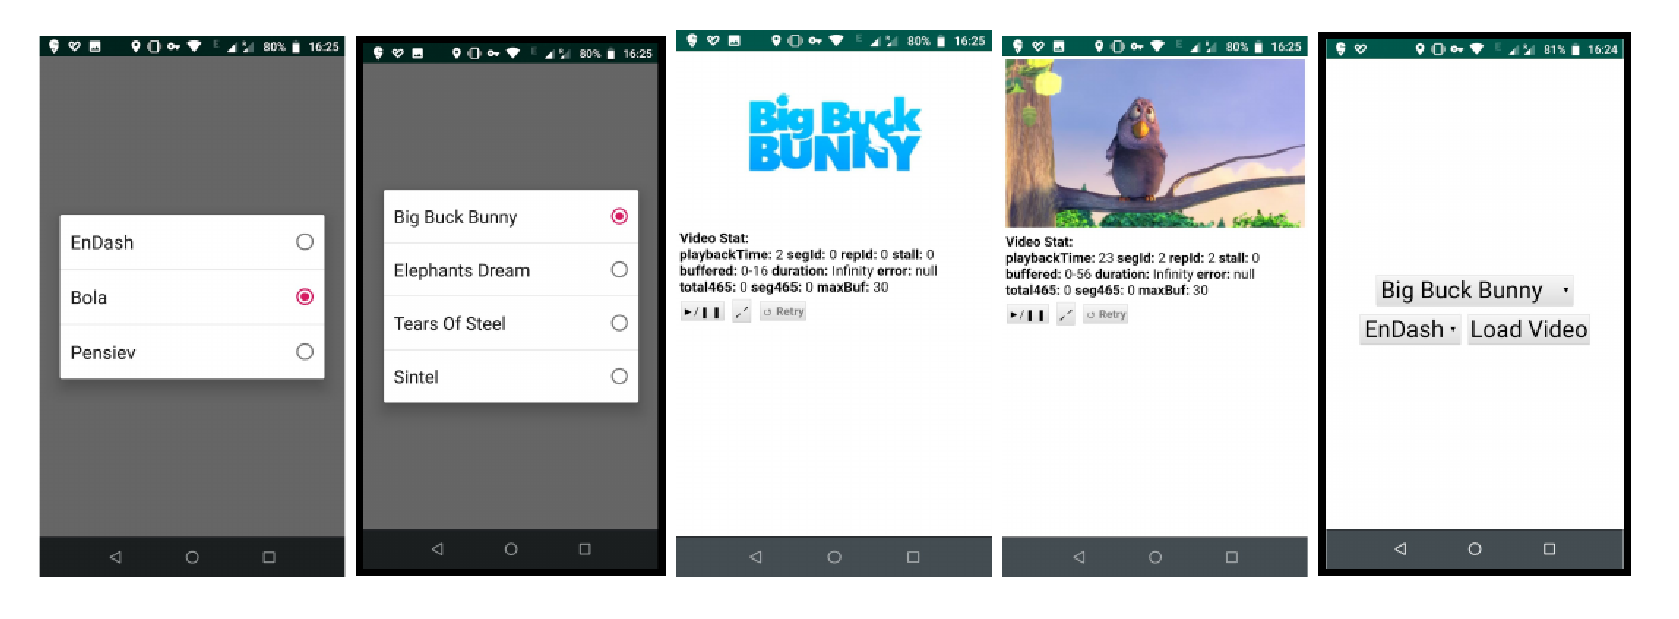
\includegraphics[width=0.8\textwidth]{images/App_Specs.eps}
    \caption{A snapshot of the \bel\ Player}
    \label{fig:chap05:bel_client}
\end{figure*}
 The heart of \bel\ is its middleware-server - \servname, which is an intelligent \ac{DASH} proxy server, It is essentially an HTTP server, albeit with a few extra capabilities. The major modules in \servname are -  a) an HTTP server,  b) a dummy client instance, and  c) the \ac{ABR} controller which houses the ABR algorithms.
\subsubsection{HTTP server}  
The \textbf{HTTP server} module forms the front end of \servname. It maintains the TCP link with the client. For ease of implementation, everytime a new request arrives, \servname\ creates a new process in the HTTP-server. This allows the utilization of the multiple cores available in the system and serve multiple requests concurrently \am{AM:(we have to mention that we have developed server using python)}.

\subsubsection{Dummy Client} 
To process the information received from the client, \servname\  creates a new instance of the client  at its end for every new service request. We refer to this instance as the dummy client. When \servname\ receives the request for the $n^{th}$ video segment download, there are two sets of information from the client - (a)  the current playback buffer status, and (b) the download information till the $(n-1)^{th}$ segment download (this can include the history for past $k$ segments. So, it generates a new server state including the aforementioned information. This is then forwarded to the \ac{ABR} controller for selecting the audio-video quality and the next sleep time duration of the client. When the bitrate decisions arrive from the \ac{ABR} controller, the dummy client instance uses the download manager to download the segment from the \ac{CDN} server. It then prepares the HTTP response, which includes (a) the downloaded segment, (b) the previous download history received from the client, and (c) the sleep time duration. 
\subsubsection{ABR Controller}  The ABR controller is a collection of pluggable ABR algorithms. The dummy controller feeds the server state containing the playback and download information to the ABR controller. These metrics are used by the \ac{ABR} algorithm placed inside the ABR controller to take the bitrate decisions. There may be different types of ABR algorithms - (i)rate based, (ii) buffer based, (iii) hybrid, i.e., both rate and buffer based, (iv) quality based, (v) learning based, etc. Some of these algorithms like~\cite{mao2017neural,Akhtar2018,Sengupta2018} needs the previous server state, in other words the download information, to calculate the output quality for the next segment.
\subsubsection{Download Manager}
Another module in the server is the \textbf{download manager} which downloads the segments from the CDN server. It also maintains a very basic LRU based caching to avoid downloading segments which have been already downloaded.
\subsection{Implementation}
The popularity of DASH, as discussed earlier, is primarily stimulated by the use of existing \ac{CDN} network and the interoperability of \ac{DASH}. In \bel\ the \ac{CDN} remains unchanged as before. In this section, we shall explain the implementation of the major modifications introduced by \bel, i.e., the \bel\ client and its \servname\ server. 

% \am{Unlike DASH, the \bel\ has three primary components 1) CDN, 2) \servname\ proxy server and 3) a \cliname. Among these three components, the CDN is exactly same as normal DASH based services. It contains the streaming data and serve to the players. The \servname\ and the \cliname\ is the splitted version of smart DASH client. Here the \cliname\ is responsible for playing the video at the end user side, however, all the decision regarding quality selection and buffer managements are taken by the \servname. In this subsection we are going to discuss the implementation detail of the \cliname\ and \servname\ and the communication protocol between these the components.} 

%\basabdatta{Need to know details from abhijit}

%\basabdatta{Need to know details from abhijit}
%\newcommand{\cliname}{dumb client}

\subsubsection{The \bel\ Client}
The \bel\ client has been developed as an HTML5 and Javascript based Android application. A snapshot of the client application is shown in Fig.2. Inside this application, the \textit{playback and buffer controller} at the client is an HTML5 video player with all playing options, such as play pause, and seek. Additionally, the video player also needs a video source, which can either be an HTTP video source or a source buffer. In this work, we use the Source buffer APIs since it offers a set of options  such as playing a video with partial data, changing video quality on the fly, etc. The  AJAX handler and the \textit{Client Controller}, which as mentioned earlier maintain the communication with \servname\  and follows and executes the instructions coming from the \servname, respectively, are both implemented using Javascript. 
\subsubsection{The \bel\ Server - \servname}
The \servname\ server has been implemented to be hosted in an Amazon Web Server. Thr front end of \servname\ is an HTTP server module which maintains the communication with the client.  It has been implemented by extending the Python BaseHTTPServer module. As Python does not support true multi-threading, a new process is created with every new request that \servname\ receives. This allows the utilization of the multiple cores available in the system and serve multiple requests concurrently. Moreover, \servname\ maintains a unique dummy client and \ac{ABR} controller for each client. This allows \servname\ to serve multiple clients at a time. When the client is on the move both the dummy client and the \ac{ABR} controller has to migrate the current \servname\ server to the new \servname, while preserving their current state.\\
\indent For implementing the ML-assisted \ac{ABR} algorithms Tensorflow is used. In this work, we have implemented only Pensieve. \basabdatta{more to write}.
\subsection{Message Flow}
\indent To render clarity to the operation of \bel\ we have shown in Fig. \ref{fig:chap05:info_xchang} the information exchanges between the \bel\ client and \servname\ in detail. Before engaging in the flow of information between the \bel\ client and the \servname\ server, we introduce a few terms - \textbf{(a) Session}: A session is the time duration from the start to the end of a single video streaming. If the player is reloaded then a new session starts. \textbf{(b) State}: A state is a set of carefully chosen parameters of an ongoing process. The criteria for the choice of parameters is to ensure that the restart point of a process should be the previous instance and not the beginning. An example of a state is the serialized object of a class. On deserialization a user will be left with an exact copy of the previous object even if the process becomes different \basabdatta{ask abhijit}. \bel\ records the states of three different modules - (a) the \bel\ client (\basabdatta{specifics}), (b) the dummy client at \servname, and (c) the ABR controller at \servname.\textbf{(c)  Download Information}: The download information is recorded at the AJAX handler and includes the payload and the header size of both the client request and the \servname\ response. It also includes three timestamps, such as, (i) request sent (\basabdatta{ask abhiit}) (ii) first byte of the response received and (iii) the last byte of the response received. The size of each download information is approximately 40 Bytes.\\
\begin{figure}[h]
    \centering
    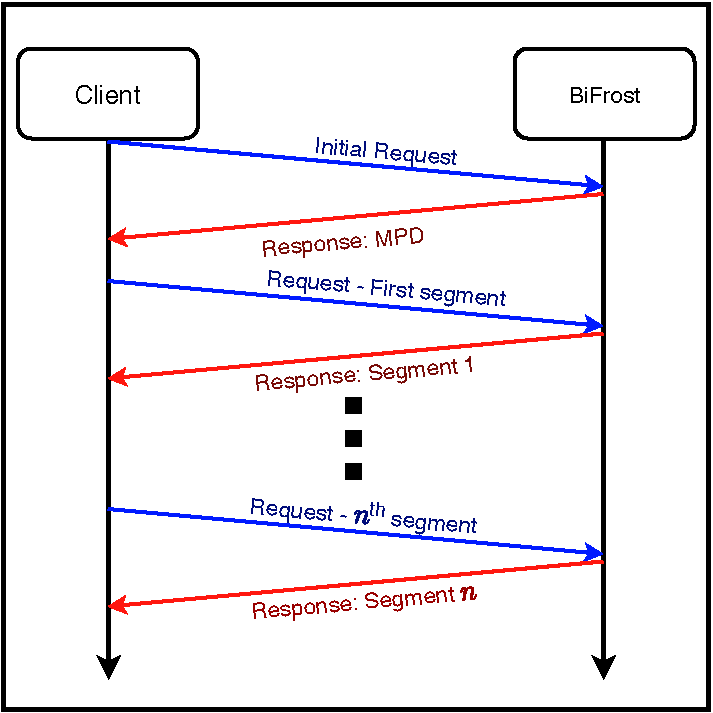
\includegraphics[width = 0.8\linewidth]{./images/splitDASHTransaction.pdf}
    \caption{The message flow between the client and the moderator server \servname\ of the \bel\ \ac{DASH} architecture. The demonstrated flow corresponds to a stateless \servname\ server. \servname\ can also be stateful.}
    \label{fig:chap05:info_xchang}
\end{figure}{}
\subsubsection{The Control Flow}
To \textit{initiate} a video streaming session the \bel\ client first places the request for the Media Presentation Description (MPD) of the target video to \servname. The MPD contains all information associated with the properties of the target video. At this stage, the playback buffer length is zero, and the \bel\ client has no download information or any information related to the video. When \servname\ receives the MPD request it creates (a) a dummy client object and (b) an \ac{ABR} object. For a non-MPD request both of these objects are either initiated with zeros or are empty. These are then piggybacked with the un-modified MPD as a blob and sent to the client.\\
\begin{figure}[h]
    \centering
    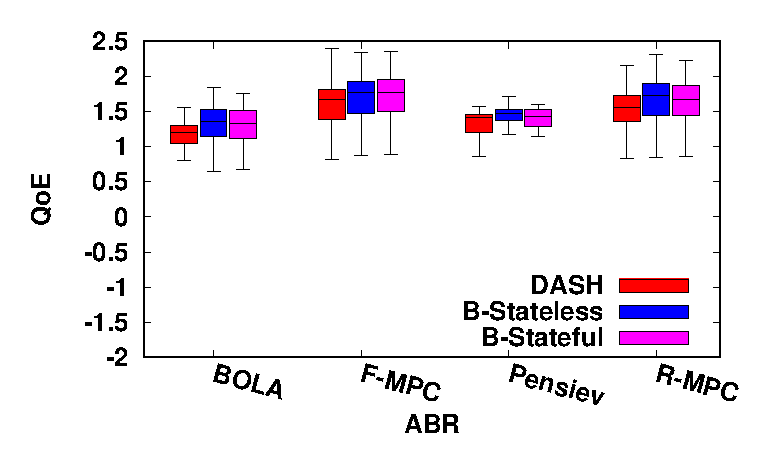
\includegraphics[width=0.5\textwidth]{images/qoeBox.eps}
    \caption{Box plot representing \ac{QoE} of users over different network conditions. The performance of both stateless and stateful \servname\ servers are captured.}
    \label{fig:chap05:result_qoe}
\end{figure}
\begin{figure}[h]
	\captionsetup[subfigure]{width=0.7\linewidth}
	\begin{center}
		\subfloat[\label{fig:chap05:result_bitrate}Average Bitrate]{
			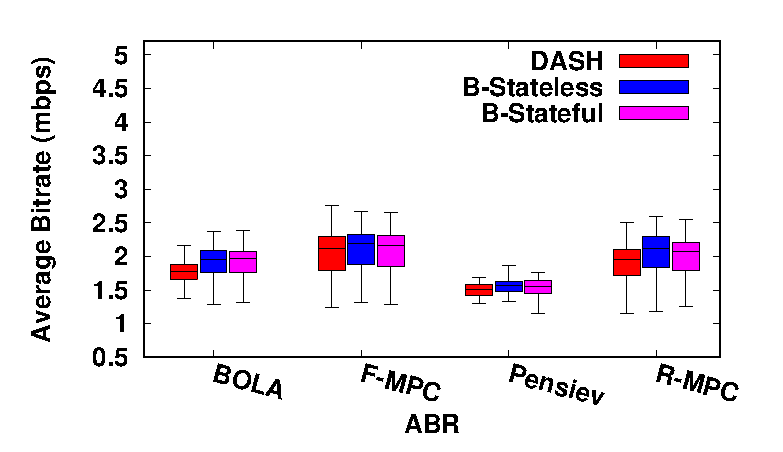
\includegraphics[width=0.49\linewidth]{images/avgQlBox.eps}
		}
%		\vspace{+5mm}
		\subfloat[\label{fig:chap05:result_smoothness}Average bitrate variation]{
			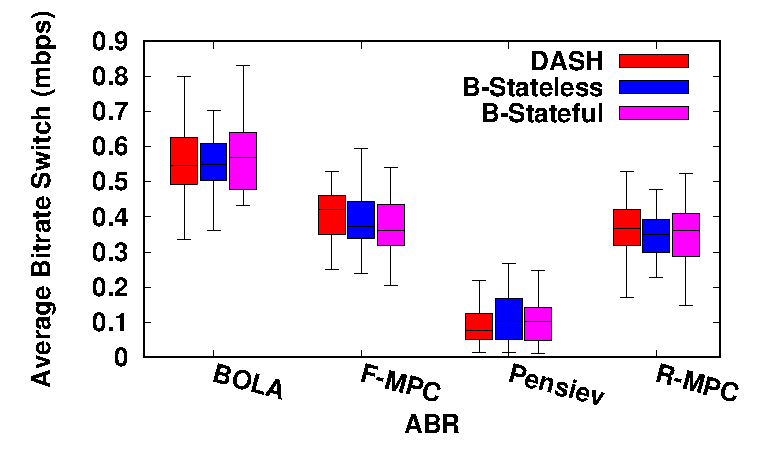
\includegraphics[width=0.49\linewidth]{images/avgQlVarBox.eps}
		}\\
%		\vspace{+5mm}
		\subfloat[\label{fig:chap05:result_stall}Average Rebufferring Time]{
			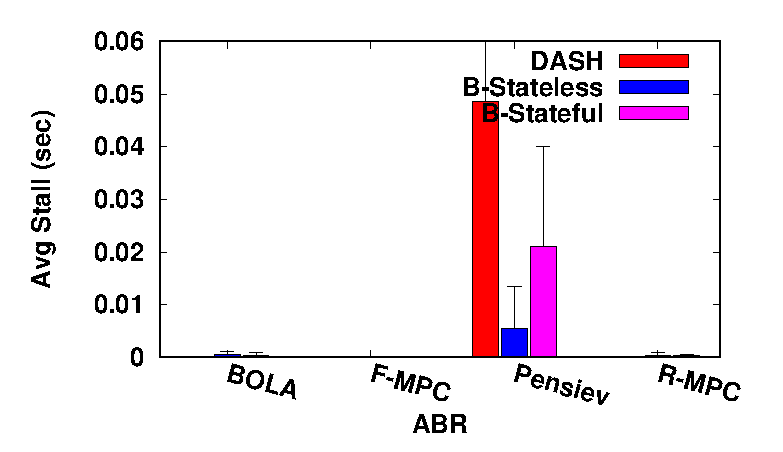
\includegraphics[width=0.3\linewidth]{images/avgStallsBox.eps}
		}
	\end{center}
	\caption{Individual QoE components}
\end{figure}
%\begin{figure*}[t]%
%\centering
%\subfigure[Average Bitrate]{%
% \label{fig:result_bitrate}%
%  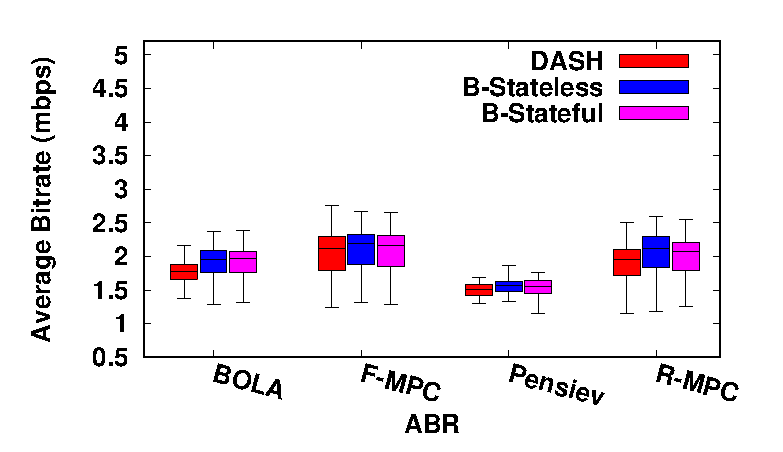
\includegraphics[width=0.3\textwidth]{images/avgQlBox.eps}}
%\hspace{0.1cm}
%\subfigure[Average bitrate variation]{%
% \label{fig:result_smoothness}%
% \includegraphics[width=0.3\textwidth]{images/avgQlVarBox.eps}
%}%
%\hspace{0.1cm}
%\subfigure[Average Rebufferring Time]{%
%\label{fig:result_stall}%
%\includegraphics[width=0.3\textwidth]{images/avgStallsBox.eps}
%}
%\caption{Individual QoE components}\vspace*{-0.5cm}
%\end{figure*}
\indent Upon receiving the MPD, the client controller records the current download information associated with the MPD, and immediately forwards the request for the first video segment download. The auxiliary information sent by the client along with the request include the playback buffer length, the playback time, the current rebuffering time  and only one download information corresponding to the MPD.  For the first request, playback buffer length, playback time, and current rebuffering time are all equal to zero. In addition it also sends the blob (containing the previous instance of the dummy client and the ABR controller at \servname) along with the request. For a non-MPD request, the dummy client state is composed of the next segment number, the download quality of the last five segments, and the last five download information. The \ac{ABR} controller state is, however, dictated by the \ac{ABR} algorithm. For example, buffer based \ac{ABR} algorithms like BOLA \cite{Spiteri2016} does not need any prior information. However, algorithms like MPC \cite{yin2015control} and Pensieve \cite{mao2017neural} require a large set of input parameters for operation \\

\indent Once the request arrives at \servname, it first looks for the blob and responds with an error if the blob is absent. Otherwise it restores the dummy client object and the ABR controller object to their previous state using the information available in the blob. Only after restoring the previous instance, it then updates both of these two objects using the new set of information received from the client. The dummy controller then directs the \ac{ABR} controller, which replies with the audio and video quality of the next video segment.  The dummy controller also calculates the time that the \bel\ client should wait before sending the next request. We refer to this as the \textit{sleep time}, which is calculated as follows:\basabdatta{write equation} Once \servname\ arrives at these decisions, it fetches the video segment from the \ac{CDN} server at the quality prescribed by the \ac{ABR} controller. It then forwards the segment along with the dummy controller and ABR controller state as well as the sleep time to the client.\\
% \indent When the client receives the segment response, it forwards it to the player. Simultaneously it updates its own sleep time. An inherent assumption is that the \bel\ client sleeps during the entire download. When the last segment is downloaded \servname\ notifies the client by sending an {\tt End of Video (EoV)} flag the client. The session terminates either if the user chooses to end the session or if the video playing is over. In the latter case, it is terminated by the client. At this stage, the playback buffer length is zero. Thus, the auxiliary information sent by the client along with first segment download request includes the playback buffer status and the MPD download information. Using both of these, the dummy client instance at \servname\ creates a server state and forwards the same to the \ac{ABR} controller. Once the \ac{ABR} controller decides the audio-video quality for the next segment download, the dummy client instance (i) downloads the segment at the corresponding quality from the \ac{CDN} server, (ii) calculates the sleep time duration, (iii) forwards the segment to the client such that the previous download history (received from the client) and the sleep time duration is piggybacked with it. For downloading the $n^{th}$ segment, the client sends the history associated with the download of $(n-1)$ segments. The client may also send the history for $(n-1-k)$ to $(n-1)$ segments for $k = {0,1,\cdots,(n-k-2}$, albeit with some minor savings in the control channel overhead.\\
% \indent The sleep time duration depends on the buffer status and the current download. It is calculated as follows:
% % \begin{enumerate}[(i)]
% %     \item 
% %     \item Upon receiving the MPD request, \servname\ prepares a new server state. It populates the state with the current download history and then  responds with an un-modified MPD for the video. If \servname\ is \textbf{stateless}, it pushes the server state to the client along with the MPD. Otherwise, if \servname\ is \textbf{stateful} then it stores the server state itself. Additionally, \servname\ also appends an identifier \textbf{X-Server-Type: Smart}, which indicates that the MPD is received from \servname\ and not the simple CDN server. This is the first instance where a bottleneck associated with the introduction of \servname\ as a middlebox is bypassed. 
% %     \item Upon reception of the MPD, the client prepares the video element in \texttt{HTML} and requests \servname\ for the first video segment. Unlike in the conventional DASH protocol, the client does not specify the video/audio quality for the segment requested. 
% %     \item When \servname\ is \textbf{stateless}, the client pushes the previous server state, containing the previous download history, along with the download request to \servname. 
% %     \begin{itemize}
% %         \item Upon reception of the request, \servname\ looks for any old state in the request. 
% %         \item If any such state is present, it expands it; otherwise, it creates a new state. 
% %         \item  In a new server state, \servname\ includes the playback information and the download history received from the client along with the request. \servname\ then feeds these information to its \ac{ABR} algorithm to calculates the best quality for both audio and video segments. 
% %     \end{itemize}
    
% %     \item In case where \servname\ is \textbf{stateful}, it stores its own previous states. So, when a new download request containing the current playback information arrives from the client, \servname\ uses the playback information and the download history in its stored server state to calculate the audio and video quality of the chunks to be fetched using an ABR algorithm.
% %     \item Once the quality is decided, \servname\ downloads the video segments at the calculated quality from the CDN/streaming (if not available in its cache) and forwards it to the client for reordering at the player. It also calculates the time for which the client should wait (i.e., the sleep time) before sending the next request to the moderator-server. It piggybacks the sleep time with the video chunks. \servname\ also adds the server state in case it has a stateless design.\basabdatta{BP: need to develop sleep time derivation formula.}
% % \end{enumerate}{}  
% %   Most of the deterministic ABR algorithms do not require to maintain any state. Hence, \servname\ by default can be designed to be stateless. However, \ac{ABR} algorithms, such as Pensieve \cite{mao2017neural}, Oboe \cite{Akhtar2018} and HotDASH \cite{Sengupta2018}, need the information on past chunk downloads to decide the bitrate of future chunks. This gives rise to the need for recording the server state of \servname. If \servname\ is stateful, amount of control information exchanged is significantly reduced. If, on the other hand, \servname\ is stateless then its storage requirement reduces, however, at the cost of increased control information exchanges. \\
%   \indent We next describe implementation aspects of the \bel\ client and the server, i.e., \servname.

% % . We have this migration in the later part of this section. 
% % server. Th recording the download information associated with every video segment download, etc. 
% % \begin{enumerate}
% % 	\item {\bf Video playback handler:} It handles the . HTML5 provides a video player and several ways to control it. The controls are like, . The video player also need a video source. The HTML5 have several options for video source like http video source, source buffer. Among these video sources, the source buffer API is particularly interesting. It allows video player to play video with partial data, change the video quality and other feature on the fly. We utilize this API to change the quality whenever require. The video playback handler module handles all these tasks.
% % 	\item {\bf AJAX handler:} The segment download manager is implemented using AJAX api available in the JavaScript. This particular module handle communication between the \cliname and the \servname and keep log in form of download inform.
% % 	\item {\bf Controller:} All though the \cliname\ is dumb, it need a controller to follow and execute instruction from the \servname. The controller module exists to perform the task. It connect the video playback handler and the the AJAX handler. It create the request to send to the \servname\ and parse the response received from the \servname.
% % \end{enumerate} 

% % \am{
% % We implement the \cliname\ using HTML5 and JavaScript. We have three basic module in our \cliname\ implementation:
% % \begin{enumerate}
% % 	\item {\bf Video playback handler:} It handles the HTML5 video player. HTML5 provides a video player and several ways to control it. The controls are like, play pause, seek. The video player also need a video source. The HTML5 have several options for video source like http video source, source buffer. Among these video sources, the source buffer API is particularly interesting. It allows video player to play video with partial data, change the video quality and other feature on the fly. We utilize this API to change the quality whenever require. The video playback handler module handles all these tasks.
% % 	\item {\bf AJAX handler:} The segment download manager is implemented using AJAX api available in the JavaScript. This particular module handle communication between the \cliname and the \servname and keep log in form of download inform.
% % 	\item {\bf Controller:} All though the \cliname\ is dumb, it need a controller to follow and execute instruction from the \servname. The controller module exists to perform the task. It connect the video playback handler and the the AJAX handler. It create the request to send to the \servname\ and parse the response received from the \servname.
% % \end{enumerate} 
% % }
% % HTML5 provides Media Source Extension (MSE) to render multi-media in the browser. It also provides an API called Source Buffer API to control the playback buffers on the fly using JavaScript. This API allows users to add segmented video chunks on the fly or to change the audio video qualities. Most of the popular browsers (including webviews) in almost all the platforms support these APIs. So, in order to make \bel\ platform independent, we have implemented the \bel\ client using HTML5 and JavaScript.\\
% %\indent In our implementation, a native HTML5 media player with MSE constitutes the video player. 



% % \subsubsection{Control flow and communication}
% % \am{
% % Before we go in depth of the control flow and communication, we like to discuss few terminologies. These are a) \textbf{session}: a session is the time from starting of video streaming to the end of the video streaming for a client. If user decide to reload the player and play the same video, it is considered as a different session. b) \textbf{State}: a state is a instance of a set of parameter of a running process. The parameters are not random rather carefully chosen in such a way that the process can be restarted from the previous instance instead of the starting point. A very good example of a state is the serialized object of a class. If one deserialize the object, he/she will get exact same copy of previous object even the processes are different. In our \bel\ system, we need to work with the states of three different modules. These are the \cliname, the dummy client and ABR controller state in the \servname. c) \textbf{Download information}: The AJAX module in \cliname captures few information related to request-response. These information contains payload and header size of both request and response and three timestamps: i) request sent, ii) first byte of the response received, iii) last byte of the response received. So the rough size of each download information is approximately 40bytes.
% % \\
% The control flow:
% \\
% \indent {\bf Initiation of a video session:} The \cliname\ initiate a video session by placing the MPD request to the \servname. At this point the \cliname\ does not have any information regarding the video. The session starts when \cliname\ receives an successful response from the \servname.
% \\
% \indent When a \servname\ receives an MPD request from a \cliname, it initiate the a dummy client object and the corresponding ABR object. The state of dummy client contains the next segment number, last five segment quality, and last five download information. The state of ABR depends on ABR itself. For example, the BOLA or buffer based ABR does not require any state to be maintain however, states of ABRs like MPC, Pensieve composed with a large set of parameters. At this point parameters in the state are either empty or initialized with zero. The \servname\ piggy back the state of the dummy client and ABR controller as blob with MPD response.
% \\
% \indent {\bf Starting playback:} Once the \cliname\ receives the MPD response, it immediately send the request for next segment i.e. first segment to the \servname. At this point the \cliname\ have only one download information and the playback buffer is empty and playback time is 0. The \cliname\ piggy back current playback time, total rebuffering time (it is zero now), playback buffer length and the only download information it have. It also add the blob it received from last request.
% \\
% \indent When a \servname\ receives segment request, it first looks for the blob in the request. It respond with error if there is no blob exist in the segment request. The \servname\ restore the dummy client object and corresponding ABR object from this blob. Once the \servname\ finally restore the objects, its update the objects with the download information, playback time and other data available with the request. At this point, the dummy client is ready to take decision like the bitrate for next segment. So, it ask the ABR controller object for the next quality and download the selected quality segment using download manager. The dummy client also calculates the time \cliname\ should wait before sending next request. When all of this decisions are made, the \servname\ piggy back the dummy client and ABR controller state as blob and send the segment data as response.
% \\
% \indent When client receives the segment response, it load the segment to the player buffer and start playing it. Simultaneously it update the sleep time it received from the \servname\ and wait for that time before sending next segment request. The sleep time needs update again because of the download delay between the \servname\ and the \cliname. We assumes that the \cliname\ was already sleeping for the download time of the segment response.
% \\
% \indent {\bf Continuations of the session:} The following segments are downloaded in exactly similar manner as the first one. The \cliname\ always last download information with the segment request.
% \\
% \indent In \servname\ side, everything continue similarly as it was for the first segment. However, The \servname\ add an {\tt End of Video (EoV)} flag with the segment response if the segment is the last segment.
% \\
% \indent {\bf Termination of the session:} The session can be terminated by an user anytime she wants by turning off the video. Otherwise the \cliname\ terminate the session once video is over. It also does not send any segment request to \servname\ once it receives an {\tt EoV} flag. It does not affect the \servname\ as \servname\ does not store any session or anything else in the server side.

\section{Evaluation}\label{sec:chap05:evaluation}
In this section we explain the evaluation methodology and subsequently present a performance comparison of the proposed \bel\ architecture with the conventional {DASH architecture}. 
\subsection{Evaluation Methodology}
The performance of \bel\ as well as the conventional \ac{DASH} have been evaluated using an emulation platform, in which the client has been implemented as a web browser application in the same computer that hosts the \servname\ server. We have used 15 network traces from the open source FCC dataset \cite{FCC2016} simulate the network between the server and the client. There are approximately 1 million throughput traces in the FCC dataset, each having a logs of average throughput over 2100 seconds with 5 second granularity. We have generated a corpus of around 15 traces each of duration 320 seconds.  The network traces have been formatted using the MahiMahi Network Emulation Tool \cite{Netravali2015}. The performance of both architectures have been evaluated by how they support each of the following four \ac{ABR} streaming algorithms - (i) BOLA \cite{Spiteri2016}, (ii) Pensieve \cite{Mao2017}, (iii) Fast-MPC \cite{Yin2015}, and (iv) Robust-MPC \cite{Yin2015}. In each architecture the performance of each of these algorithms have been evaluated by streaming four open source videos, Big buck bunny (10:53 seconds), Sintel (14 minutes 48 seconds),  Tears of Steel (12 minutes 12 seconds) and Elephants Dream (10 minutes 53 seconds). These videos have been encoded at seven different bitrate levels and a video chunk is of eight seconds duration. For a given network trace, each of these videos has been streamed once using one \ac{ABR} algorithm in each architecture. Thus, for a single ABR algorithm, a performance metric is calculated from the combined outcomes of these four videos  in a given architecture. For example, the \ac{QoE} box corresponding to the BOLA algorithm in the \bel\ architecture in Fig: \ref{fig:chap05:result_qoe} includes the combined performance statistics of the aforementioned videos when streamed using BOLA. If there are $N$ network traces and $V$ videos, then the box includes the $N\times V$ data for BOLA in the \bel\ architecture. The same is true for Fig. 5.
\subsection{Performance Comparison}
Fig. \ref{fig:chap05:result_qoe} shows the QoE supported by different algorithms in the proposed \bel\ architecture as well as the \ac{DASH} architecture. Fig. 5 shows the individual QoE components. It is seen for almost all algorithms that \bel\  performs at par and sometimes even better than the existing DASH architecture. The reason for this can be attributed to the increase in computation accuracy offered by the \servname\ server. Nevertheless, the stateless design of \bel\ comes with some increase in control channel overhead. To bypass this problem, \bel\ can be designed to be stateful, in which case the blob containing the state of the dummy controller object and the ABR object is not forwarded to the client. Instead, it is saved at the server. The corresponding performance evaluated in terms of the \ac{QoE} metrics and their individual components is also shown in Fig. \ref{fig:chap05:result_qoe} and Fig. 5. It can be inferred from these figures that the stateful \bel\ design performs equally well as its stateless counterpart, albeit with reduced control channel overhead but with some increase in the storage requirements. In the stateful design the blob has to be transferred from one \servname\ server to another for supporting mobility.\\
\indent Thus, the \bel\ architecture emerges as a suitable alternative to the \ac{DASH} architecture which offers increased feasability for running ML-assisted \ac{ABR} algorithms. Nevertheless, it can also be used for non-ML \ac{ABR} algorithms with equal efficiency. 
% \begin{figure}
%     \centering
%     \includegraphics[width=0.5\textwidth]{images/avgQlBox.eps}
%     \caption{Average Bitrate}
%     \label{fig:result_bitrate} ot
% \end{figure}
% \begin{figure}
%     \centering
%     \includegraphics[width=0.5\textwidth]{images/avgQlVarBox.eps}
%     \caption{Average bitrate variation}
%     \label{fig:my_label}
% \end{figure}
% \begin{figure}
%     \centering
%     \includegraphics[width=0.5\textwidth]{images/avgStallsBox.eps}
%     \caption{Rebuffering Time}
%     \label{fig:result_stall}
% \end{figure}
\section{Discussion}\label{sec:chap05:discussion}
\section{Conclusion}\label{sec:chap05:conclusion}
%\begin{enumerate}
%     \item \textcolor{red}{Motivation results needed}
%     Demonstration of the fact that client side does not always have necessary information
%     \item usefulness of stateless and stateful in case of handover
%     \item Results for explaining stall
% \end{enumerate}
% \begin{itemize}
%     \item Directly hit the point - ML based algos too many; we have tried to understand how much the ML based algos are adaptive and feasible for wide scale deployment
%     \item Move to the problems - suggest initial solution
%     \item initial solution at client split with a portion in the server - all this in first para
%     \item second stanza - implications at the system level
%     \item since complete overhauling - middlebox justification
%     \item middlebox indispensable - so where will be architectural changes; should be enumerated very clearly
%     \item how much of this can be mitigated
%     \item USP - not splitdash, but system implications of implementation: main objective and/or focus
%     \item by default stateful
%     \item Why was DASH implemented in the client side? highest penetration of HTTP/HTTPs. Large number of CDNs deployed - difficult to change, better change to client side
%     \item Less control with the client??? 
%     \item Any compromize with existing DASH philosophy? If not, then strongly justify
%     \item architecture being made more flexible without compromising on DASH philosophy
%     \item WIFI-cellular handover - discussion towards the end
% \end{itemize}


\clearemptydoublepage

\chapter{Federated Adaptive Bitrate Live Streaming over Locality Sensitive Playback Coalitions}
\label{chapter06}
\noindent

\renewcommand{\relpath}[1]{Chapters/06.FLiDASH/}
\graphicspath{{Chapters/06.FLiDASH/}}

\newcommand{\our}{FLiDASH}

%\section{Introduction}
%During the last decade, social video streaming for targeted audiences have seen a huge boom with applications like Twitch.tv, Periscope, Meerkat along with the traditional YouTube \& Facebook live and similar other personalized live streaming services~\cite{wang2016anatomy}. Live broadcasts over such platforms have increased many-folds during the recent COVID-19 pandemic due to over-the-top (OTT) services like online live broadcast of classroom lectures to the students\footnote{\url{https://www.nokia.com/blog/network-traffic-insights-time-covid-19-march-23-29-update/} (Accessed: \today)}. Many existing studies indicate that live streaming of popular events, such as a live cricket or football match, creates multiple traffic bottlenecks in the network, particularly at the Internet gateways of private organizational networks or Internet Service Providers (ISP)~\cite{yan2018understanding}. Consequently, a question arises -- how can we prevent traffic bottlenecks in the Internet while allowing high definition video streaming to millions of users? 

In the previous chapters, we have analyzed the online video streaming systems and developed a way to reduce the energy consumption while streaming online videos. In this chapter, we consider a class of live but non-interactive streaming applications, where the video is broadcast to a set of targeted audiences over social streaming applications. Social streaming applications many-a-times form communities which are localized, forming one or more geographical clusters~\cite{wang2016anatomy}. We utilize this localized community formations among live streaming viewers to construct one or more playback coalitions, as shown in \fig\ref{fig:chap06:flsd}. The coalition members share a common network gateway (such as an organizational local network gateway or the service gateway for a cellular core network) to connect to the Internet, however, there are direct high-speed local connections among the coalition members (like \acr{LAN} connections or cellular device-to-device connections). It can be noted that such a coalition can be formed based on the principles of \ac{ALTO}, where an \ac{ALTO} server can provide the locality information of video players without requiring any explicit network or device firmware change. The coalition members collectively download the video from the content provider based on an \ac{ABR} streaming strategy, such as \ac{DASH}. The clients in a coalition collectively decide the adaptive playback rate and share data-download loads among themselves maintaining the playback synchronization. 
\begin{figure}[!ht]
    \centering
    \includegraphics[width=0.8\linewidth]{img/flsd.pdf}
    \caption{Overview of \our: The clients under a local network create a coalition, every members of the coalition share the total download load.}
    \label{fig:chap06:flsd}
\end{figure}

However, developing such a system has multiple challenges. First, the coalition needs to be designed in a way such that downloading data directly from the content provider is costlier than sharing the data over the local network. Second, there should be a proper distribution of segment-wise data-download scheduling among the coalition members such that playback synchronization is not violated. A proper playback synchronization ensures that every player in the coalition should acquire the video segment $s_{i}$, either downloaded by itself or fetched from another coalition player through the direct local link, by the time it completes playing the previous video segment $s_{i-1}$; otherwise, there might be a rebuffering delay affecting the \ac{QoE}. Third, the Internet bandwidth of individual players may vary over time; therefore, the coalition as a whole should schedule the video segment downloads among its members as well as decide the bitrate of every video segment based on the \ac{ABR} principle.

Owing to the above challenges, we develop a coalition-based adaptive live streaming  called \textit{Federated Live Streaming over \ac{DASH}} (\our) where the streaming clients or players form a dynamic coalition based on the network quality parameters and collectively stream a live video. We use the playback buffer statistics at individual streaming clients to develop a distributed mechanism for coalition formation with the help from a proximity server (which can be an \ac{ALTO} server). The members of a coalition use a low-overhead gossip-based protocol for playback synchronization and takes following two decisions -- (1) scheduling the downloads of video segments among the coalition members based on their individual instantaneous network condition and the overall fairness criteria, and (2) bitrate of each video segments to optimize the overall \ac{QoE} of the coalition. We use the following \ac{QoE} objectives while making the above decisions -- (a) improve the overall video quality level, (b) improve the playback smoothness by reducing the quality fluctuations, (c) reduce rebuffering, and (d) improve fairness  among the coalition members in terms of the downloaded data share. We have implemented {\our} over an emulated environment and have thoroughly compared its performance with various other baselines. We observe that {\our} improves the overall \ac{QoE} with less traffic overhead at the backbone network.

The rest of the chapter is organized as follows. 


%\section{Related Work}
There are few works in the literature like \textit{DASH over Information Centric Networking} (ICN)~\cite{ICN-DASH} and \textit{Multicast ABR}~\cite{multicastAbrCablelabs}, which use adaptive bitrate in a collaborative setup. All the segments of a DASH video contain a unique name through the URL. ICN provides a way to get the contents based on a name, and thus the DASH video segments can be routed according to the name. In case of a ICN, if the video players are behind a common ICN gateway, the gateway can cache the DASH video segments based on the unique name, and thus, can reduce duplicate delivery of contents. However, ICN needs significant changes in the network architecture including its routing policies, and thus, is not readily deployable on the existing networks. In 2016, Cablelabs introduced multicast ABR (M-ABR)~\cite{multicastAbrCablelabs} to provide the same video content to a large group of viewers while ensuring low network overhead via IP multicast. In M-ABR, all the ISPs maintain an M-ABR device that gets connected to the original video server. The M-ABR device receives the data from the video content server and then uses IP multicast to forward the content to the end-users. However, in this architecture, the content provider needs to push a middlebox (M-ABR server) to the ISP. Further, there needs to be a software change at the client devices. There exist few works in the literature to take care of the ABR selection over a collaborative setup, however, in these systems, the video players need to coordinate with an Internet middlebox that works as a central controller, such as a tracker~\cite{detti2016tracker}, a software controller~\cite{khalid2019sdn} or the cloud~\cite{payberah2012clive,wang2014migration}. This limits the scalability as all the video players need to coordinate with the controller for each ABR decisions which are taken for every video segment requests. In contrast to such existing approaches, {\our} works without the support from any such Internet middleboxes. 


\section{Split-DASH System Architecture}
The DASH or DASH like system provides a way (guideline) to change video quality instead of pausing a video streaming during bad network quality. There are several implementation of the DASH or DASH like streaming system and most of them have a HTML5 based implementation using {\it Media Source Extension}(MSE)\cite{wiki:dash,w3c:mse}. These implementations also support {\it Digital Right Management}(DRM) via {\it Encrypted Media Extension}(EME)\cite{w3c:eme}. These implementation have several modules implemented either in {\it Javascript} or in browser. The modules like playback, media decryption are implemented in browser or some browser extension/plugin (\ie Widevine plugin for DRM protection). The different modules are as follows:

{\bf Playback module} or the player is the module which actually render the video. It is implemented mostly in the browser. It is mostly implemented in the browser and render in a html element. The player is accessed and controlled via MSE APIs.

{\bf Buffer controller} manages and monitor video buffer. It is partly implemented using javascript and partly by the browser itself.

{\bf Adaptive bitrate controller} is the module decides the quality based on the network condition. It can have multiple algorithm and implemented in javascript it self. It is the most crucial part of DASH like streaming system yet the most flexible part. Any streaming provider can implement there won algorithm based on their requirement. We will discuss more about ABR later part of the article.

{\bf Download manager} is responsible for downloading the segment/chunk chosen by the ABR algorithm. It monitors the progress of ongoing downloads to gain fine tune information about the network condition. Most of the time it download chunk using AJAX (Asynchronous JavaScript And XML)


{\bf CDN/Streaming Servers} are http based static file server. It contains all the data requires to play a video smoothly.

{\bf DRM protection module:} It provides DRM protection using EME when a streaming provider wants to protect the right of content. It is an independent component and does not influence the ABR algorithm or other components. DRM protection module is out of the scope of this work.

\begin{figure}[ht]
   \begin{center}
           \includegraphics[width=0.7\linewidth]{img/playerDiagram_basic}
   \end{center}
   \caption{\label{fig:playerDiagram_basic} Original DASH based streaming system.}
\end{figure}

The inter-connection of the modules are depicted in the Fig.~\ref{fig:playerDiagram_basic}. Here, the ABR controller controls the playback via buffer controller while instructing download manager to download appropriate segment in the appropriate time. The ABR controller is the most important component. There are active research going on to improve ABR controller. As ABR controller is the part of the player, it need to be implemented in client application it self. In case HTML based player, ABRs need to be implemented in javascript. The ABR algorithm like MPC\cite{dash:mpc}, BOLA\cite{dash:bola} or the algorithms described in \cite{dash:probe,dash:cs2p,dash:CFA,dash:rnb,dash:buffer} does not have any special library requirement and can be implemented easily in any technology. However, as machine learning based ABR algorithm like Pensieve\cite{dash:pensieve}, OBOE\cite{dash:oboe} or HotDASH\cite{dash:hotdash} need specialized machine learning (ML) library and very hard to implement if the technology does not have support for required library. So, it is very difficult to deploy these algorithm in browser based video player.

\begin{figure}[ht]
	\begin{center}
		\includegraphics[width=0.7\linewidth]{img/playerDiagram_ml}
	\end{center}
	\caption{\label{fig:playerDiagram_ml} Modified DASH based streaming system to support ML based ABR algorithm}
\end{figure}

Authors of the ML based algorithm show prototype by modifying the system little bit. The new dash based video system looks like Fig.~\ref{fig:playerDiagram_ml}. Here they propose to replace the ABR controller in the client with a dummy one and run a ABR server in the local system. Every time, the player need to take a decision, dummy ABR controller contact ABR server with the current state of the player. The ABR server response the decision based on the algorithm of its choice.

The advantage of this system is that it does not depends on the client technology. ABR server can be implemented in any technology it suit best. However, it involves a extra communication with a external server which may be fatal to the viewing experience if the round trip time between the player and the ABR server. To avoid the communication delay between the player and ABR server, the ABR server need to run in local system only. This system is not easy to deploy as it need to a ABR server of each and every player.

\subsection{Split-DASH architecture}
\label{sec:Split_DASH_architecture}
To solve above problem we propose Split-DASH architecture. In split-DASH architecture, we split the original DASH architecture into two parts, i) a dumb player or client and ii) a smart server side. The proposed architecture depicted in the Fig.~\ref{fig:playerDiagram_split}.
\begin{figure}[ht]
	\begin{center}
		\includegraphics[width=0.9\linewidth]{img/playerDiagram_split}
	\end{center}
	\caption{\label{fig:playerDiagram_split} Modified DASH based streaming system to support ML based ABR algorithm}
\end{figure}
Here we make the player dumb. It controls the play back but it do not take any decision. Instead it depends on the decision provided by the smart part counter part in the server. The server provides the following decision: i) time to download a segment, and ii) quality of the segment. Before we explain functionality of different modules in the server and client, we explain the transaction between dumb-client and the smart server. 

\begin{figure}[h]
	\begin{center}
		\includegraphics[width=0.5\linewidth]{img/splitDASHTransaction}
	\end{center}
	\caption{\label{fig:splitDASHTransaction} Modified DASH based streaming system to support ML based ABR algorithm}
\end{figure}

The Fig.~\ref{fig:splitDASHTransaction} depict the transaction between smart proxy server and dumb client. At first client request the Media Presentation Description (MPD) from the server. The smart proxy server returns a un-modified MPD for the video. However, it also adds a server identifier {\tt X-Server-Type: Smart}. This identifier indicate that the server is not simple CDN server, instead, it is a smart proxy server. So, the dumb client prepare the HTML video element and request for the first video segment. Here client does not mention the video/audio quality for the segment. Instead, client enclose the download history with the request. When the server receives a request, it looks for old server state in the request. If present, it will expand the state, other wise, it create a new state. Then, update the state according to the current playback information and download history provided in the request. Based on this information, server calculate the best quality for both audio and video segment based on the pre-decided ABR algorithm. Once quality is decided, it download the required segments of the calculated quality from the CDN/streaming (if not available in it cache) and send it back to the dumb player. It Also calculate the time player should wait (i.e. sleep time) before sending another request to the server. It multiplexes the sleep time and server state with the request. The contents of the server state is dependent of the ABR algorithm. Most of the deterministic ABR algorithm, does not required to maintain any state, however, ABR algorithm like pensieve need to maintain state. In case of pensieve, server state contains only the pensieve state.
Here we send server state to client to make server stateless. The client does not read the server state, however, it store it and send with next request.

\noteam{need to add overhead with a table or plot}


\section{SpEnDASH Architecture}
Recently we have developed a energy aware DASH based ABR algorithm EnDASH for smartphones. The algorithm is described in \noteam{cite/ref algo here}. The EnDASH algorithm heavily dependent on smartphone sensor data and neural-network driven ABR algorithm. We implement the EnDASH by modifying Split-DASH architecture (\ref{sec:Split_DASH_architecture}). We call it SpEnDASH architecture. The SpEnDASH architecture have 3 parts, i) A android application, ii) Modified split-DASH dumb client and iii) EnDASH aware smart proxy server. Fig.~\ref{fig:playerDiagram_SpEnDASH} describe the different components and interactions between those components. In this model, entire video playback system run inside a webview in an android application. The application collect several informations regarding the device and feed to the webview. The dumb player running inside the webview collect those data and send them to the server with the segment request. The server store those use all the informations to find out the next video quality using the EnDASH algorithm and return the response accordingly.
\begin{figure}[h!]
	\begin{center}
		\includegraphics[width=0.9\linewidth]{img/playerDiagram_SpEnDASH}
%		\includegraphics[width=0.9\linewidth]{img/playerDiagram_split}
	\end{center}
	\caption{\label{fig:playerDiagram_SpEnDASH} Modified DASH based streaming system to support ML based ABR algorithm}
\end{figure}

{\bf Advantages:}

\section{Evaluation}
To evaluate our proposed streaming system, we compare \textit{CoaliDASH} with existing streaming systems and adaptation algorithms. Apart from \textit{CoaliDASH}, we have implemented two different streaming systems under the environment module --  {\it Simple} and {\it DHT based}. The {\it Simple} environment emulates the DASH based client-server adaptive streaming where we have used three baselines -- BOLA~\cite{bola2-acm-mmsys2018}, MPC~\cite{MPC-SIGCOMM-2015} and Pensieve~\cite{Pensieve}.  The {\it DHT} environment represents an environment with a distributed hash table based peer-to-peer system \cite{ChordStoica,dht1}.
%\notesc{Give a citation for DHT.} 
All the above streaming clients have been implemented in Python\footnote{The source code of the implementation is available publicly at the following link -- \url{https://github.com/abhimp/CoaliDASH}} and has been executed over an emulation environment as discussed next. 
%Our proposed algorithm is based on collaborative segment downloading. It important to have a large set of players in the network, otherwise it falls back as a standalone player with BOLA as the ABR. It is difficult to have such a big network in a real environment, and it is more difficult to configure such a big network with different network condition. To avoid all these issues, we emulate the streaming player on top of a simulated environment.

\subsection{Emulation Environment}
\label{sec:simulatorprop}
We develop a emulator platform similar to~\cite{Pensieve} to analyze the performance of \textit{CoaliDASH} under diverse environments. The developed emulation environment has the following features. All the players in the system have access to system clock which is an event-driven clock handled by the emulator core. The emulator uses a reference network to define the connectivity across the networked nodes; where every node of the network runs a streaming player. The network characteristics (bandwidth, delay between two nodes) of the reference network has been used to configure the network characteristics of the emulated network. We maintain a global playback time; the streaming server does not reveal any informations about a segment unless that segment can be downloaded according to the global playback time. We use Mahimahi \cite{mahimahi} network traces to emulate the network condition of the links between video server to a player, based on the reference network. We have randomly assigned different Mahimahi traces to every player in a network. The emulated player can use any existing ABR implementation without any modification as long as it takes the player-state as the input and gives the next segment quality as the output. 
%	\item The simulator can emulate a network if it runs with a reference network. It places a player per node of the reference network.
%	\item Any Two players in the system communicate only through the emulated network. For the emulated network, simulator needs a reference network which will provide the bandwidth delay between two nodes. We calculate communication delay carefully and a conservative way so that it does not violets the real communications between delay. For TCP like communication between two play in the simulated network, we calculate the transmission time based the delay and sender buffer. It is not accurate, but it gives higher transmission time than our empirical studies.
%	\item A player will never access the future video information. We maintain a global playback time. The video server module will never reveal any informations about a segment unless that segment can be downloaded according to the global playback time.
%	\item We use Mahimahi \cite{mahimahi} like network trace to simulate the network condition of the links between video server to a player. We randomly assigned different Mahimahi traces to every player in a network.
%	\item The emulated player can use any existing ABR implementation without any modification as long as it takes the player state as input and gives next segment quality as the output. This feature eliminates the possibility of faulty implementation.
%\end{itemize}
In the emulated environment, we use Eq.~(\ref{eqn:transmissionTime}) to compute the transmission time $T_{ij}$ between two players $P_i$ and $P_j$ in a coalition. Here $clen$ is the data length of the video segment, $d_{ij}$ is delay between two nodes, $buf$ is the sender buffer and $x$ is the noise factor which is uniformly distributed between $\theta_1$ to $\theta_2$. 
%\notesc{What is $P(x)$?}
\begin{align}
T_{ij} = clen\times \frac{buf}{2\times d_{ij}} \times x \mbox{\hspace{1cm}}& \theta_1 <= x <= \theta_2  
%& \mathcal{p}(x) = \frac{1}{\theta_2 - \theta_1} 
\label{eqn:transmissionTime}
\end{align}



%
%\begin{figure}[ht]
%	\captionsetup[subfigure]{}
%	\begin{center}
%		\subfloat[\label{fig:avgBitratebox} Averge Bitrate]{
%			\includegraphics[width=0.49\linewidth]{img/grpbasic/avgbitrate_box_1}
%		}
%		\subfloat[\label{fig:avgBitratecmf}Average Bitrate]{
%			\includegraphics[width=0.49\linewidth]{img/grpbasic/avgbitrate_cdf_1}
%		}
%	\end{center}
%	\caption{\label{fig:avgBitrate} Average bitrate played}
%\end{figure}



%\begin{figure}[ht]
%	\captionsetup[subfigure]{}
%	\begin{center}
%		\subfloat[\label{fig:avgBitrateVarbox}]{
%			\includegraphics[width=0.49\linewidth]{img/grpbasic/avgbitrate_var_box_1}
%		}
%		\subfloat[\label{fig:avgBitrateVarcmf}]{
%			\includegraphics[width=0.49\linewidth]{img/grpbasic/avgbitrate_var_cdf_1}
%		}
%	\end{center}
%	\caption{\label{fig:avgBitrateVar} Average bitrate variation during playback}
%\end{figure}




%As we discussed at \ref{sec:simulatorprop}, we designed all this environment carefully so that it emulates real network condition and does not take any unfair advantage of the fact that everything is directly accessible. We use BOLA as the base ABR for every environment if not specified otherwise. We compared our system with BOLA, MPC and Pensieve ABR. We use the implementation provided by Pensieve source code directly for BOLA, MPC and Pensieve. The {\it Simple} environment was used as the environment while experimenting with BOLA, MPC and Pensieve. Although we run experiments with both RobustMPC, we have shown only RobustMPC results of RobustMPC as results are almost the same. As BOLA, MPC and Pensieve are ABR for the single player streaming system, we implement DHT as a baseline of the peer-to-peer system.

\subsection{Experimental Setup}
We run our emulation with a large set of autonomous system data available from SNAP database~\cite{ASDataSet} as reference networks. We have executed the systems over 710 reference networks, with 100 to 1000 nodes per network. As mentioned earlier, every network node runs a streaming client. To train the model for learning based adaptive streaming like Pensieve~\cite{Pensieve}, we use $58$ DASH-ified videos with a total duration of $45$ hours. We have taken only lengthy videos for our experiment because most of the live online live streaming lasts more than one hour \cite{LiveStreamDuration1,LiveStreamDuration2}. We have created Mahimahi compatible traces from publicly available dataset, like a broadband trace from FCC~\cite{dataset-fcc} and the 3G/HSDPA mobile dataset collected in Norway~\cite{dataset-norway}. We modified these datasets as described in \cite{Pensieve} to make it Mahimahi compatible.

For experimentation, we use the QoE definition as given in \cite{Pensieve}. According to this definition, we consider three QoE components -- (i) average quality level, (ii) average jump in the quality level (smoothness of the video playback) and (iii) re-buffering time. Let $\mathcal{Q}_n$ denote the quality level for video segment $n$ and $\mathcal{T}_n$ be the re-buffering time. Considering that there are $N$ number of segments in a reference video, the average QoE is defined as follows. 
\begin{equation}
QoE = \frac{\alpha}{N}\sum_{n=0}^{N} \mathcal{F}(\mathcal{Q}_n) - \frac{\beta}{N-1} \sum_{n=1}^{N}\lvert\mathcal{F}(\mathcal{Q}_n) -\mathcal{F}(\mathcal{Q}_{n-1})\rvert - \gamma\mathcal{T}_n
\label{eqn:QoE}
\end{equation}
Here, $\alpha$, $\beta$ and $\gamma$ are weight factors (values between 0 and 1) to individual components, such that $\alpha + \beta + \gamma = 1$. 


%\begin{figure}[h]
%	\captionsetup[subfigure]{}
%	\begin{center}
%		\subfloat[\label{fig:Stall_Timebox}]{
%			\includegraphics[width=0.49\linewidth]{img/grpbasic/stalltime_box_1}
%		}
%		\subfloat[\label{fig:Stall_Timecmf}]{
%			\includegraphics[width=0.49\linewidth]{img/grpbasic/stalltime_cdf_1}
%		}
%	\end{center}
%	\caption{\label{fig:Stall_Time}Total stall time observed each player}
%\end{figure}
%
%\begin{figure}[h]
%	\captionsetup[subfigure]{}
%	\begin{center}
%		\subfloat[\label{fig:QoEbox}]{
%			\includegraphics[width=0.49\linewidth]{img/grpbasic/qoe_box_1}
%		}
%		\subfloat[\label{fig:QoEcmf}]{
%			\includegraphics[width=0.49\linewidth]{img/grpbasic/qoe_cdf_1}
%		}
%	\end{center}
%	\caption{\label{fig:QoE}Quality of experience (linear)}
%\end{figure}


\begin{figure}[ht]
	\captionsetup[subfigure]{}
	\begin{center}
		\subfloat[\label{fig:avgBitratecmf}Average Bitrate]{
			\includegraphics[width=0.49\linewidth]{img/grpbasic/avgbitrate_cdf_1}
		}
     	\subfloat[\label{fig:avgBitrateVarcmf}Bitrate Variation]{
     			\includegraphics[width=0.49\linewidth]{img/grpbasic/avgbitrate_var_cdf_1}
     		}
	\end{center}
	\caption{\label{fig:avgBitrate} QoE Components: Average Bitrate and Bitrate Variation}
\end{figure}

\subsection{Results}
We first observe the individual QoE components for \textit{CoaliDASH} in comparison with other baselines. Fig.~\ref{fig:avgBitratecmf} compares the average playback bit-rate for various streaming applications. In Fig.~\ref{fig:avgBitrateVarcmf}, we show the variation in average playback bit-rates, which indicate the smoothness of the video rendering. We observe that the performance of BOLA in terms of average playback bit-rate is very low, and most of the players played the videos in lower average quality compared to other baselines. BOLA is very conservative about the bitrate, whereas it is much concerned about the re-buffering time. Pensieve and MPC improve the video quality compared to BOLA by utilizing reinforcement learning and deep inspection, respectively. DHT is the first system which uses the knowledge of existing players in the network and form a peer-to-peer architecture for collectively download the videos. So, it improves the average video quality compared to client-server based ABR. However, CoaliDASH clusters the players based on their network conditions and render the videos keeping the coalition members in sync. In Fig.~\ref{fig:avgBitratecmf}, it is clear that there are clusters of players who play a video in almost equal quality levels. Although we observe that the average variation in the video quality is higher for CoaliDASH; however, it is because the deviation of video quality levels among various coalitions. A coalition where majority of the members have low network resources, the average quality of the video gets drop down. 
%A slight change in the quality incurs high variation.

\begin{figure}[!ht]
	\captionsetup[subfigure]{}
	\begin{center}
		\subfloat[\label{fig:Stall_Timecmf}Total Re-buffering Time]{
			\includegraphics[width=0.49\linewidth]{img/grpbasic/stalltime_cdf_1}
		}
       	\subfloat[\label{fig:QoEcmf}Overall QoE]{
       			\includegraphics[width=0.49\linewidth]{img/grpbasic/qoe_cdf_1}
       		}
	\end{center}
	\caption{\label{fig:avgBitrateVar} Re-buffering Time and Overall QoE}
\end{figure}

Next, Fig.~\ref{fig:Stall_Timecmf} compares the total re-buffering time among various baselines. We observe that the re-buffering time is very high for DHT because it needs more time to search for a video segment from the network before it can fetch it directly from the streaming server. The re-buffering time for CoaliDASH is moderated although it includes the skip time during the synchronization among the members of the coalition. BOLA incurs almost no re-buffering time; whereas Pensieve and MPC suffer from noticeable re-buffering time. As the re-buffering time is a significant contributor in the overall QoE measurement (Eq.~(\ref{eqn:QoE})), the overall QoE for various baselines, as shown in Fig.~\ref{fig:QoEcmf}, indicates that \textit{CoaliDASH} outperforms other baselines in term of maximum achievable QoE.  Among the various scenarios simulated over our developed platform, more than $50\%$ of the cases, \textit{CoaliDASH} incurs a high QoE (value between $2$--$4$). 

\begin{figure}[!ht]
	\captionsetup[subfigure]{}
	\begin{center}
		\subfloat[\label{fig:cdnuploaded_byte} Data downloaded from the server]{
			\includegraphics[width=0.49\linewidth]{img/grpbasic/cdnupload_1}
		}
		\subfloat[\label{fig:cdnuploaded_cnt} \# of segment downloads from the server]{
			\includegraphics[width=0.49\linewidth]{img/grpbasic/cdnuploadcnt_1}
		}
	\end{center}
	\caption{\label{fig:cdnuploaded}Streaming Server Usages}
\end{figure}

One of the major objectives of \textit{CaliDASH} is to reduce the usage of streaming server when multiple co-located streaming players play the same live video. In Fig.~\ref{fig:cdnuploaded}, we plot the streaming server usage by different baselines in terms of the total bytes downloaded from the streaming server and the number of video segments directly downloaded from the streaming server. We observe that that the streaming server usages by DHT is lowest. In the case of CoaliDASH, players are bounded to receive data from its group only, while in case of DHT, a player can share segments with as many players as possible. The standalone players need to download all the segments directly from the server. Therefore, we observe a performance trade-off here -- \textit{CoaliDASH} significantly improves the QoE performance while having little increase in the streaming server load. In a nutshell, the proposed approach makes a balance between the QoE and streaming server load during the peer-assisted live video streaming.  


%Fig.~\ref{fig:avgBitrate}, \ref{fig:avgBitrateVar}, \ref{fig:Stall_Time} and \ref{fig:QoE} we report the general result we found from our experiment. Fig.~\ref{fig:QoE} is a plot of Quality of Experience. We calculate QoE using the Equation~\ref{eqn:QoE}. In the equation, $\alpha$ is the quality factor and $\beta$ and $\gamma$ are smoothness penalty and stall penalty.
%
%
%
%According to Fig.\ref{fig:avgBitrate} performance of BOLA very low and most of the players played in lower quality. BOLA is very conservative about the bitrate and very much concerned about the rebuffering time. Pensieve and MPC improved the video quality compared to the BOLA by utilising reinforcement learning and deep inspection respectively. DHT is the first system which uses the knowledge of existing players in the network. So, it improves an average video quality compared to ABR. However, CoaliDASH clustered the players and played video in sync. In Fig.~\ref{fig:avgBitratecmf}, it is clear that there are clusters of players who played video in almost equal quality. Average variation in video quality is higher for CoaliDASH. However, it is higher because it played in the video in high quality. A slight change in the quality incurs high variation.


%\begin{figure}[h]
%\captionsetup[subfigure]{}
%\begin{center}
%	\subfloat[\label{fig:benfit_bitrate} Benefit in terms of average bitrate]{
%		\includegraphics[width=0.49\linewidth]{img/grpbasic/benefit_bitrate_box_1}
%	}
%	\subfloat[\label{fig:benefit_qoe} Benefit in terms of QoE]{
%		\includegraphics[width=0.49\linewidth]{img/grpbasic/benefit_qoe_box_1}
%	}
%\end{center}
%\caption{\label{fig:benefit}Per player benefit of using CoaliDASH}
%\end{figure}



\begin{figure*}[h]
	\captionsetup[subfigure]{}
	\begin{center}
		\subfloat[\label{fig:grp_qoe}Overall QoE]{
			\includegraphics[width=0.33\linewidth]{img/grpbasic/grpsz_qoe}
		}
		\subfloat[\label{fig:grp_download}Amount of Data Upload and Download]{
			\includegraphics[width=0.33\linewidth]{img/grpbasic/grpsz_upload_download}
		}
       	\subfloat[\label{fig:grp_fairness}Fairness]{
       			\includegraphics[width=0.33\linewidth]{img/grpbasic/grpsz_fairness}
       		}
	\end{center}
	\caption{\label{fig:grpsz}Effect of Coalition Size}
\end{figure*}





%\subsection{Benefit of using CoaliDASH}
%In Fig.~\ref{fig:benefit}, we report the benefit of using CoaliDASH instead of another streaming system for each player in the system. Here we plot only two metrics, i.e. average bitrate and QoE. To measure the benefit of using CoaliDASH we need to keep the environment (i.e. network condition) of a player same for each ABR and reference network. It is possible for because our environment is simulated and the entire simulation state depends on the initial random variable\footnote{We use pseudo-random variable available in {\tt python numpy} library. It generates the same sequence of random numbers for the same seed/initial state.} state. However, it means that every time we run the experiment with the same environment, ABR and reference network, we get the same result. For this reason, we do not run the same experiment with the same environment, ABR and network. However, to measure the benefit of using CoaliDASH instead of other ABR, we run an experiment on a large set of environments and reference network. We use Equation~\ref{eqn:benefit} to compute the benefit of a single player. Here $G_g$ is the metric for using CoaliDASH and $G_o$ is the same metric for other ABR. We plot all the benefit as a box plot. Here benefit $Ben(S)==0$ means CoaliDASH performed precisely the same as the other ABR. The positive and negative benefit means the better or worse performance of CoaliDASH compared to other ABR.
%\begin{equation}
%Ben(S) = \frac{G_g - G_o}{|G_o|}
%\label{eqn:benefit}
%\end{equation}
%From Fig.~\ref{fig:benefit}, we can see that most of the player in the experiments gain some forms of benefit in terms of average playback quality as well as the QoE. The slight degradation in the benefit in terms of QoE with compared to BOLA. We have already seen in the Fig.\ref{fig:QoE} that QoE of BOLA is very high although the average quality is low because of its very low stall time. However, the overall performance of CoaliDASH is higher than any other existing ABR or systems.
%\subsection{Effect of group size}
In all the previous experiments, we have fixed the maximum coalition size to 4 players. Here we check the effect of the increasing the coalition size. Fig.~\ref{fig:grp_qoe} and Fig.~\ref{fig:grp_download} shows the impact of different coalition sizes on the overall QOE and the total amount of data downloaded from the streaming server, respectively. We observe that a large coalition size provides better QoE because it gives more time to download a segment. However, in the case of a large coalition, every player has to upload more data to the other members of the coalition, which incurs an additional overhead.

%\subsection{Fairness}
In collaborative scenario, fairness among the members is an important metric. In our evaluation, we measure the fairness among the coalition members using Jain fairness index on QoE among the players \cite{jain1999throughput}. We measure the fairness among players in two categories, i) intra-coalition fairness (fairness among the coalition members of a coalition) and ii)inter-coalition fairness (fairness among the coalitions). The results are reported in Fig.~\ref{fig:grp_fairness}. We have computed fairness for seven different coalition sizes. Here we observe that the intra-coalition fairness index is always close to 1, which indicates a perfect fairness. However, inter-coalition fairness is not very high. It is expected as different coalitions can play video in different video quality which has a major contribution to the overall QoE. 
%From this result, we can conclude that CoaliDASH is fair.


\section{Conclusion}
\label{chap03sec:conclusion}

In this work, we studied the internal working of YouTube's bitrate adaptation algorithm, by identifying important parameters and exploring their roles.
We observed that YouTube adapts segment length in addition to quality level, a behavior not been reported earlier.
As an implication, we observed that data wastage for a playback session is significantly lower than estimated previously.
We further provided an analytical model, augmented with a machine learning based classifier, to predict data consumption in adavance for a video playback session.
As an immediate future direction, we would like to explore other important implications of segment length adaption for YouTube.

\clearemptydoublepage


%\begin{appendix}
%\chapter[Extended results of Chapter]
\noindent

%
%\end{appendix}

\renewcommand{\bibname}{References}
\bibliographystyle{abbrv}
%\bibliographystyle{unsrt}
%\bibliographystyle{alpha}
%\bibliography{ref/thesis,ref/collection,ref/others}
\bibliography{ref/ieee,ref/acm,ref/springer,ref/sciencedirect,ref/usenix,ref/mix,ref/rfc}
%\bibliography{ref/all}

\addcontentsline{toc}{chapter}{Dissemination}
\chapter*{Dissemination}
\vspace*{0.5cm}
% \noindent
\renewcommand{\chaptermark}[1]{\markboth{}{\sffamily #1}}
\chaptermark{Dissemination}
\begin{center}
\textbf{\underline{Journals}}
\end{center}
\begin{enumerate}
\item journal 1
\end{enumerate}

\begin{center}
{\textbf{\underline{Conferences}}}
\end{center}
% \subsection*{Conferences}

\begin{enumerate}
\item conf 1

\end{enumerate}
% \endgroup
\noindent
% \rule{0.49\textwidth}{0.75pt} $_{\Diamond}$ \rule{0.49\textwidth}{0.75pt}\\

% \end{onehalfspacing}





\clearemptydoublepage


\end{document}
